% **************************************************
% Document Class Definition
% **************************************************
\documentclass[%
	paper=A4,					% paper size --> A4 is default in Germany
	twoside=true,				% onesite or twoside printing
	openright,					% doublepage cleaning ends up right side
	parskip=full,				% spacing value / method for paragraphs
	chapterprefix=true,			% prefix for chapter marks
	11pt,						% font size
	headings=normal,			% size of headings
	bibliography=totoc,			% include bib in toc
	listof=totoc,				% include listof entries in toc
	titlepage=on,				% own page for each title page
	captions=tableabove,		% display table captions above the float env
	draft=false,				% value for draft version
]{scrreprt}%

% **************************************************
% Debug LaTeX Information
% **************************************************
%\listfiles

% **************************************************
% Information and Commands for Reuse
% **************************************************
\newcommand{\thesisTitle}{Bounded Sceptical Reasoning}
\newcommand{\thesisName}{Isabelly Lour�do Rocha}
%\newcommand{\thesisSubject}{Human Reasoning}
\newcommand{\thesisDate}{November 6th, 2017}
%\newcommand{\thesisVersion}{Version 1}

\newcommand{\thesisFirstReviewer}{Prof. Dr. Steffen H�lldobler}
\newcommand{\thesisFirstReviewerUniversity}{\protect{Technische Universit�t Dresden, Germany}}
\newcommand{\thesisFirstReviewerDepartment}{Department of Computer Science}

\newcommand{\thesisSecondReviewer}{Prof. Dr. Sergio Tessaris}
\newcommand{\thesisSecondReviewerUniversity}{\protect{Free University of Bolzano, Italy}}
\newcommand{\thesisSecondReviewerDepartment}{KRDB Research Centre for Knowledge Representation}

\newcommand{\thesisFirstSupervisor}{Prof. Dr. Steffen H�lldobler}

\newcommand{\thesisUniversity}{\protect{Technische Universit�t Dresden}}
\newcommand{\thesisUniversityDepartment}{Department of Computer Science}
\newcommand{\thesisUniversityInstitute}{International Center for Computational Logic}
\newcommand{\thesisUniversityGroup}{Knowledge Representation and Reasoning Group}
\newcommand{\thesisUniversityCity}{Dresden}
\newcommand{\thesisUniversityStreetAddress}{N�thnitzer Strasse 46}
\newcommand{\thesisUniversityPostalCode}{01187}
\usepackage[list=true,listformat=simple]{subcaption}% FOR SUBTABLES
\newcommand{\CalA}{\mathcal{A}}
\newcommand{\CalC}{\mathcal{C}}
\newcommand{\CalP}{\mathcal{P}}
\newcommand{\CalO}{\mathcal{O}}
\newcommand{\CalM}{\mathcal{M}}
\newcommand{\CalN}{\mathcal{N}}
\newcommand{\CalE}{\mathcal{E}}
\newcommand{\CalF}{\mathcal{F}}
\newcommand{\CalH}{\mathcal{H}}
\newcommand{\CalG}{\mathcal{G}}
\newcommand{\CalS}{\mathcal{S}}
\newcommand{\CalT}{\mathcal{T}}
\newcommand{\CalL}{\mathcal{L}}
\newcommand{\CalI}{\mathcal{I}}
\newcommand{\CalJ}{\mathcal{J}}
\newcommand{\CalIC}{{\cal IC}}
\newcommand{\Next}{\textit{next}\xspace}
\newcommand{\Done}{\textit{done}\xspace}
\newcommand{\inputtreshold}{\frac{1}{2}}
\newcommand{\hiddentreshold}{\frac{\omega}{2}}
\newcommand{\outputtreshold}{\frac{\omega}{2}}
\newcommand{\noessay}{e^\bot}
\newcommand{\library}{\ell^\top}
\newcommand{\nolibrary}{\ell^\bot}
\newcommand{\abone}{\Ab_1^\top}
\newcommand{\noabone}{\Ab_1^\bot}
\newcommand{\abtwo}{\Ab_2^\top}
\newcommand{\noabtwo}{\Ab_2^\bot}
\newcommand{\textbook}{t^\top}
\newcommand{\notextbook}{t^\bot}
\newcommand{\essay}{e^\top}
\newcommand{\Def}{\mathit{def}}
\newcommand{\Undef}{\mathit{undef}}
\newcommand{\Atoms}{\mathit{atoms}}
\newcommand{\Comp}{\mathit{c}}
\newcommand{\WComp}{\mathit{wc}}
\newcommand{\ModelsWCS}{\models_{\normalfont\textit{wcs}}}
\newcommand{\udf}{\mbox{\normalfont U}}
\newcommand{\Body}{\mbox{\em Body}}
\newcommand{\Lfp}{\mathsf{lfp}\,}
\newcommand*{\DashedArrow}[1][]{\mathbin{\tikz [baseline=-0.25ex,-latex, dashed,#1] \draw [#1] (0pt,0.5ex) -- (1.3em,0.5ex);}}%
  % ABBREVIATIONS FILE
% **************************************************
% Load and Configure Packages
% **************************************************
\usepackage[utf8]{inputenc}		% defines file's character encoding
\usepackage[english]{babel} % babel system, adjust the language of the content
\usepackage[					% clean thesis style
	figuresep=colon,%
	sansserif=false,%
	hangfigurecaption=false,%
	hangsection=true,%
	hangsubsection=true,%
	colorize=full,%
	colortheme=bluemagenta,%
	bibsys=bibtex,%
	bibfile=bib-refs,%
	bibstyle=numeric,%
]{cleanthesis}
%\usepackage{algorithm2e}
\usepackage{algorithmic}
\renewcommand{\algorithmicrequire}{\textbf{Input:}}
\renewcommand{\algorithmicensure}{\textbf{Output:}}
\renewcommand{\algorithmicwhile}{\textbf{Function}}
\renewcommand{\algorithmicendwhile}{\textbf{EndFunction}}
\usepackage{booktabs}
\usepackage{tikz} % FOR FIGURES
\usetikzlibrary{decorations.markings} 
\usetikzlibrary{snakes} 
\usepackage{forest}
\usepackage{amsmath}
\usepackage{amsthm}
\usepackage{tcolorbox}
\usepackage{xpatch}
\usepackage[nogroupskip,toc,acronym,style=long]{glossaries}
\makeatletter
\xpatchcmd{\proof}{\@addpunct{.}}{\@addpunct{:}}{}{}
\makeatother
\usetikzlibrary{shapes,positioning,arrows,backgrounds,fit,calc,automata}  
% !TEX root = ../thesis.tex
% ------------------------------------------------------------------------------------------------------------------------------------------------------------ %
\newcommand{\NetworkAP}[1][]{% 1 optional parameter for options for the tikz picture
%TIKS BEGIN
\def\layersep{1.5cm}
\def\networkini{4.0cm}
\def\networky{1}
\def\networkinisk{8.8}
\def\netx{1}
\def\nety{1}
\def\sep{1.5}
\def\sepx{\distancelayers}
%\resizebox{0.6\textwidth}{!}{%
\begin{tikzpicture}[
              connection/.style={inner sep=0,outer sep=0}
transition/.style={rectangle,draw=black!50,fill=black!20,thick,
inner sep=0pt,minimum size=40mm},
shorten >=1pt,->,draw=black!50, node distance=\layersep]
\draw [fill = lightgray];
  \tikzstyle{every pin edge}=[-,shorten <=1pt]
%\tikzstyle{every pin edge}=[0pt]    
%\tikzstyle{neuron}=[circle,fill=black!25,minimum size=12pt,inner sep=0pt]
\tikzstyle{input}=[box,draw=gray!80,,minimum size=12pt,inner sep=0pt,text width=2em, text centered]
\tikzstyle{neuron}=[circle,draw=gray!80,,minimum size=12pt,inner sep=0pt,text width=2em, text centered]    
\tikzstyle{or neuron}=[neuron]; %, fill=gray!50 ,fill=black!25
\tikzstyle{and neuron}=[neuron];  %, fill=gray!20
\tikzstyle{annot} = [text width=2em, text centered]

% Draw the input layer nodes
\node[neuron, label=above:$d$] (inputzero) at (\netx-8,\nety)  {\tiny$\frac{\omega}{2}$};

% \coordinate[above right of=inputzero] (out);
% 
% \draw[black] (inputzero.north) to  (out);

\node[neuron, label=above:$n$] (inputone) at (\netx-4,\nety)  {};
\node[neuron, label=left:$q_0$, , fill=lightgray] (inputtwo) at (\netx,\nety-1)  {$\inputtreshold$};


\path[black] (inputzero.north) -- coordinate[midway] (mqz) (inputzero.south);
\draw [black]  (inputzero.north) to[out=20,in=-50,looseness=3.2]  (inputzero.south);

\draw[black,-] (inputone.south) to[out=-100,in=-40,looseness=0.7] ($(mqz) + (0.55,-0.45)$);
\fill ($(mqz) + (0.55,-0.45)$) circle (2pt);

\node[neuron, label=right:$\essay$] (abdessay) at (\netx+4,\nety-2.5)  {$\outputtreshold$};
\node[neuron, label=right:$\noessay$] (abdnoessay) at (\netx+4,\nety-4)  {$\outputtreshold$};
\node[neuron, label=right:$\textbook$] (abdtext) at (\netx+4,\nety-5.5)  {$\outputtreshold$};
\node[neuron, label=right:$\notextbook$] (abdnotext) at (\netx+4,\nety-7)  {$\outputtreshold$};

%hidden


\node[neuron, label=left:$q_1$] (hidden1) at (\netx,\nety-2.5)  {$\hiddentreshold$};
\node[neuron, label=left:$q_2$] (hidden2) at (\netx,\nety-4)  {$\hiddentreshold$};
\node[neuron, label=left:$q_3$] (hidden3) at (\netx,\nety-5.5)  {$\hiddentreshold$};
\node[neuron, label=left:$q_4$] (hidden4) at (\netx,\nety-7)  {$\hiddentreshold$};
\node[neuron, label=left:$q_5$] (hidden5) at (\netx,\nety-8.5)  {$\hiddentreshold$};
\node[neuron, label=left:$q_6$] (hidden6) at (\netx,\nety-10)  {$\hiddentreshold$};
\node[neuron, label=left:$q_7$] (hidden7) at (\netx,\nety-11.5)  {$\hiddentreshold$};
\node[neuron, label=left:$q_8$] (hidden8) at (\netx,\nety-13)  {$\hiddentreshold$};


% \draw [black]  (inputone.east) to [out=-45,in=-150,looseness=1]  (inputtwo.west);

\draw[black] (inputtwo.south) to (hidden1.north);

\draw [black]  (hidden1.south) to (hidden2.north);
\draw [black]  (hidden2.south) to (hidden3.north);
\draw [black]  (hidden3.south) to (hidden4.north);
\draw [black]  (hidden4.south) to (hidden5.north);
\draw [black]  (hidden5.south) to (hidden6.north);
\draw [black]  (hidden6.south) to (hidden7.north);
\draw [black]  (hidden7.south) to (hidden8.north);
% \draw [black]  (hidden8.east)  to[out=-180,in=200, edge node={node [sloped,above]} , looseness=0.25]  (inputone.west);


% \draw[black] (hidden8.south) .. controls ($ (hidden8) - (8,3)$)
% and ($ (inputtwo) + (-0.5,-0.5)$) .. (inputtwo.west);

\coordinate[below left of=hidden8] (cont);

\draw[black,rounded corners=10pt, -] (hidden8.south) |- (cont);
\draw[black,rounded corners=50pt] ($(cont) + (0.5,0)$) -| (inputzero.south);

\draw[black] (hidden8.south)  to[out=-25,in=40,looseness=1]  (inputtwo.north);

\draw[black,shorten >= -0.5pt, shorten <= -0.5pt] (inputtwo.south) to[out=-100,in=-140,looseness=3.2] (inputtwo.west) node (L1) {};


\path[black] (inputtwo.south) -- coordinate[midway] (mq0) (inputtwo.west);


\path[black,shorten >= -0.5pt, shorten <= -0.5pt] (hidden1.south) -- coordinate[midway] (mq1) (hidden1.west);
\path[black] (hidden2.south) -- coordinate[midway] (mq2) (hidden2.west);
\path[black] (hidden3.south) -- coordinate[midway] (mq3) (hidden3.west);
\path[black] (hidden4.south) -- coordinate[midway] (mq4) (hidden4.west);
\path[black] (hidden5.south) -- coordinate[midway] (mq5) (hidden5.west);
\path[black] (hidden6.south) -- coordinate[midway] (mq6) (hidden6.west);
\path[black] (hidden7.south) -- coordinate[midway] (mq7) (hidden7.west);
\path[black] (hidden8.south) -- coordinate[midway] (mq8) (hidden8.west);

% \draw[black] (inputone.east)  to[out=-70,in=-190, looseness=0.8]  node {}( $(hidden1)!0.45!(inputtwo) $ );

\draw[black,-] (inputone.south) to[out=-70,in=-190, looseness=0.6]   ($(mq0) - (0.4,0.3)$.west);
\fill ($(mq0) - (0.4,0.3)$.north) circle (2pt);


\draw[black,-] (inputone.south) to[out=-70,in=-190, looseness=0.6]   ($(mq1) - (0.4,0.3)$.west);
\fill ($(mq1) - (0.4,0.3)$.north) circle (2pt);

\draw[black,-] (inputone.south) to[out=-70,in=-190, looseness=0.6]   ($(mq2) - (0.4,0.3)$.west);
\fill ($(mq2) - (0.4,0.3)$.north) circle (2pt);

\draw[black,-] (inputone.south) to[out=-70,in=-190, looseness=0.6]   ($(mq3) - (0.4,0.3)$.west);
\fill ($(mq3) - (0.4,0.3)$.north) circle (2pt);

\draw[black,-] (inputone.south) to[out=-70,in=-190, looseness=0.6]   ($(mq4) - (0.4,0.3)$.west);
\fill ($(mq4) - (0.4,0.3)$.north) circle (2pt);

\draw[black,-] (inputone.south) to[out=-70,in=-190, looseness=0.6]   ($(mq5) - (0.4,0.3)$.west);
\fill ($(mq5) - (0.4,0.3)$.north) circle (2pt);

\draw[black,-] (inputone.south) to[out=-70,in=-190, looseness=0.6]   ($(mq6) - (0.4,0.3)$.west);
\fill ($(mq6) - (0.4,0.3)$.north) circle (2pt);

\draw[black,-] (inputone.south) to[out=-70,in=-190, looseness=0.6]   ($(mq7) - (0.4,0.3)$.west);
\fill ($(mq7) - (0.4,0.3)$.north) circle (2pt);

\draw[black,-] (inputone.south) to[out=-70,in=-190, looseness=0.6]   ($(mq8) - (0.4,0.3)$.west);
\fill ($(mq8) - (0.4,0.3)$.north) circle (2pt);


\draw[black,shorten >= -0.5pt, shorten <= -0.5pt] (inputone.south)  to[out=-50,in=-215, looseness=1.2]  node {} ( $(inputtwo) + (0.3,0.7)$ );


\draw[black,shorten >= -0.5pt, shorten <= -0.5pt] (inputone.south)  to[out=-70,in=-180, looseness=0.8]  node {} ( $(hidden1)!0.42!(inputtwo)$ );

\draw[black,shorten >= -0.5pt, shorten <= -0.5pt] (hidden1.south)  to[out=-100,in=-140,looseness=3.2] node {} (hidden1.west);
\draw[black,shorten >= -0.5pt, shorten <= -0.5pt] (inputone.south)  to[out=-70,in=-180, looseness=0.8]  node {} ( $(hidden2)!0.42!(hidden1)$ );


\draw[black,shorten >= -0.5pt, shorten <= -0.5pt]  (hidden2.south)  to[out=-100,in=-140,looseness=3.2]  node {} (hidden2.west);
\draw[black,shorten >= -0.5pt, shorten <= -0.5pt]  (inputone.south)  to[out=-70,in=-180, looseness=0.8]  node {}( $(hidden3)!0.42!(hidden2) $ );

\draw[black,shorten >= -0.5pt, shorten <= -0.5pt]  (hidden3.south)   to[out=-100,in=-140,looseness=3.2] node {} (hidden3.west);
\draw[black,shorten >= -0.5pt, shorten <= -0.5pt] (inputone.south)  to[out=-70,in=-180, looseness=0.8]  node {}( $(hidden4)!0.41!(hidden3) $ );
 
\draw[black,shorten >= -0.5pt, shorten <= -0.5pt]  (hidden4.south)   to[out=-100,in=-140,looseness=3.2]  node {} (hidden4.west);
\draw[black,shorten >= -0.5pt, shorten <= -0.5pt] (inputone.south)  to[out=-70,in=-180, looseness=0.8]  node {}( $(hidden5)!0.41!(hidden4) $ );

\draw[black,shorten >= -0.5pt, shorten <= -0.5pt] (hidden5.south)  to[out=-100,in=-140,looseness=3.2] node {} (hidden5.west); 
\draw[black,shorten >= -0.5pt, shorten <= -0.5pt]  (inputone.south)  to[out=-70,in=-180, looseness=0.8]  node {}( $(hidden6)!0.41!(hidden5) $ );

\draw[black,shorten >= -0.5pt, shorten <= -0.5pt]  (hidden6.south) to[out=-100,in=-140,looseness=3.2]  node {} (hidden6.west);
\draw[black,shorten >= -0.5pt, shorten <= -0.5pt]  (inputone.south)  to[out=-70,in=-180, looseness=0.8]  node {}( $(hidden7)!0.41!(hidden6) $ );
 
\draw[black,shorten >= -0.5pt, shorten <= -0.5pt]  (hidden7.south)  to[out=-100,in=-140,looseness=3.2] node {} (hidden7.west);
\draw[black,shorten >= -0.5pt, shorten <= -0.5pt]  (inputone.south)  to[out=-70,in=-180, looseness=0.8]  node {}( $(hidden8)!0.41!(hidden7) $ );

\draw[black,shorten >= -0.5pt, shorten <= -0.5pt]  (hidden8.south)  to[out=-100,in=-140,looseness=3.2]  node {} (hidden8.west);


% hidden to output

 \draw[black,shorten >= -0.5pt, shorten <= -0.5pt] (hidden1.south) to[out=0,in=-195, looseness=1.2] (abdessay.west);
\draw[black,shorten >= -0.5pt, shorten <= -0.5pt]  (hidden2.south) to[out=0,in=-180, looseness=1.2] (abdnoessay.west);
\draw[black,shorten >= -0.5pt, shorten <= -0.5pt]  (hidden3.south) to[out=0,in=-180, looseness=1.2](abdtext.west);
\draw[black,shorten >= -0.5pt, shorten <= -0.5pt]  (hidden4.south) to[out=0,in=-180, looseness=1.2](abdnotext.west);

 \draw[black,shorten >= -0.5pt, shorten <= -0.5pt] (hidden5.south) to[out=-40,in=-190, looseness=1] (abdessay.west);
 \draw[black,shorten >= -0.5pt, shorten <= -0.5pt] (hidden6.south) to[out=-20, in=-170, looseness=0.7](abdessay.west);
%  
%  
 \draw[black,shorten >= -0.5pt, shorten <= -0.5pt] (hidden7.south) to[out=-20,in=-180, looseness=0.6] (abdnoessay.west);
 \draw[black,shorten >= -0.5pt, shorten <= -0.5pt] (hidden8.south) to[out=-10, in=-180, looseness=0.4](abdnoessay.west);
%  
  \draw[black,shorten >= -0.5pt, shorten <= -0.5pt] (hidden5.south) to[out=-40,in=-180, looseness=1.2] (abdtext.west);
 \draw[black,shorten >= -0.5pt, shorten <= -0.5pt] (hidden6.south) to[out=-30, in=-180, looseness=1](abdnotext.west);
%  
%  
 \draw[black,shorten >= -0.5pt, shorten <= -0.5pt] (hidden7.south) to[out=-20,in=-180, looseness=0.8] (abdtext.west);
 \draw[black,shorten >= -0.5pt, shorten <= -0.5pt] (hidden8.south) to[out=-10, in=-180, looseness=0.6](abdnotext.west);
 
 
% borders

\coordinate[below right=7cm and -1cm of abdnotext] (cornerRightDown)  {};

\coordinate[below left=1cm and 1cm of inputzero] (cornerLeftUp)  {};


%\draw [-,dotted, gray]  (inputzero.east) to (inputone.west);
%\draw [-,dotted, gray, rounded corners = 5pt]  (inputone.east) -| (abdessay.north);
%\draw [-,dotted, gray]  (abdessay.south) to (abdnoessay.north);
%\draw [-,dotted, gray]  (abdnoessay.south) to (abdtext.north);
%\draw [-,dotted, gray]  (abdtext.south) to (abdnotext.north);

%\draw [-,gray, dotted, rounded corners = 5pt] (cornerRightDown) -| (abdnotext);

%\draw [-,gray, dotted, rounded corners = 5pt]  (cornerRightDown) -| (cornerLeftUp);

% \draw [-,gray, rounded corners = 5pt] (cornerLeftUp) |-  (cornerRightDown);
%\draw[-,gray, rounded corners = 5pt, dotted] (cornerLeftUp) |- (inputzero);

\node[align = center, below left=6cm and 8.7cm of abdnotext] {$\CalN_{\CalA_{\CalP_1}}$};

\end{tikzpicture}

} 
% !TEX root = ../thesis.tex

\newcommand{\NetworkAPExtension}[1][]{% 1 optional parameter for options for the tikz picture

\begin{tikzpicture}[trim left=-15cm]%[shorten >=1pt,->,draw=black!50, node distance=\layersep]

\tikzstyle{annot} = [text width=4em, text centered]
\tikzstyle{neuron}=[circle,draw=black,,minimum size=12pt,inner sep=0pt,text width=2em, text centered]     

%%% Nodes %%%
\node[neuron] (D) at (-4,3) {$d$};
\node[neuron] (T) at (-1,3) {$n$};
\node[neuron] (E) at (2,3) {$e$};
\path[] (E) edge [loop left,thick] node {} (E);

\foreach \id in {0,...,4}
	\node[neuron] (Q-\id) at (-8,-4*\id) {$q_\id$};

\foreach \id in {5,...,8} {
	\pgfmathtruncatemacro\y{\id-4};
	\node[neuron] (Q-\id) at (4*\id-24,-4*\id) {$q_\id$};
	\node[neuron] (H-\id) at (8,-4*\y) {$h_\id$};
	\path[] (H-\id) edge [loop above,thick] node {} (H-\id);
}

%%% Connections %%%
\foreach \id in {0,...,3} {
	\pgfmathtruncatemacro\y{\id+1};
	\draw [black, ->]  (Q-\id.south) to (Q-\y.north);
}

\foreach \i in {4,...,7} {
	\pgfmathtruncatemacro\k{\i+1};
	\foreach \j in {\k,...,8} {
		\pgfmathtruncatemacro\y{-4*\i};
		\draw plot [smooth, tension=0.6,->] coordinates { (4*\i-24,\y-0.4) (4*\i-22,-4*\j)  (4*\j-24.4,-4*\j)};
	}
}

\draw plot [smooth, tension=0.6,->] coordinates {  (-8,0.4) (-7.6,2.5) (-4.4,3)};

\draw [->, black, rounded corners = 10pt] (-4,3.4) to (-4,4) to (7,4) to (7,-3.3) to (7.8,-3.3);
\fill (7.8,-3.3) circle (2pt);
\draw [->, black, rounded corners = 10pt] (-4,3.4) to (-4,4) to (7,4) to (7,-7.3) to (7.8,-7.3);
%\draw plot [smooth, tension=0.4,->] coordinates {  (-4,3.4) (-3,5) (6,4) (7,-6) (7.8,-7.3)};
\fill (7.8,-7.3) circle (2pt);
\draw [->, black, rounded corners = 10pt] (-4,3.4) to (-4,4) to (7,4) to (7,-11.3) to (7.8,-11.3);
%\draw plot [smooth, tension=0.4,->] coordinates {  (-4,3.4) (-3,5) (6,4) (7,-10) (7.8,-11.3)};
\fill (7.8,-11.3) circle (2pt);
\draw [->, black, rounded corners = 10pt] (-4,3.4) to (-4,4) to (7,4) to (7,-15.3) to (7.8,-15.3);
%\draw plot [smooth, tension=0.4,->] coordinates {  (-4,3.4) (-3,5) (6,4) (7,-13.5) (7.8,-15.3)};
\fill (7.8,-15.3) circle (2pt);


%Unit t%
\draw[black,->] (T.south) to[in=-10,out=-90, looseness=0.3] (-8,-2);
\draw[black,->] (T.south) to[in=-10,out=-90, looseness=0.3] (-8,1.5);

\draw[black,->] (T.south) to[in=-10,out=-90, looseness=0.3] (-1,-4);
%\draw[black,-] (T.south) to[in=-10,out=-90, looseness=0.3] (-5,-4.7);

\draw[black,->] (T.south) to[in=-10,out=-90, looseness=0.3] (-2,-8);
%\draw[black,-] (T.south) to[in=-10,out=-90, looseness=0.3] (-5,-9.4);

%\draw[black,-] (T.south) to[in=-10,out=-90, looseness=0.3] (-5,-10.6);
\draw[black,->] (T.south) to[in=-10,out=-90, looseness=0.3] (-4,-12);

%\draw[black,-] (T.south) to[in=-10,out=-90, looseness=0.3] (-5,-14.6);
\draw[black,->] (T.south) to[in=-10,out=-90, looseness=0.3] (-7,-16);

\draw[black,-] (T.south) to[in=-10,out=-90, looseness=0.3] (1.1,3);
\fill (1.1,3) circle (2pt);

%Unit e%
\draw[black,-] (E.south) to[in=-10,out=-90, looseness=0.3] (-8,-2.5);
\fill (-8,-2.5) circle (2pt);
\draw[black,->] (E.south) to[in=-10,out=-90, looseness=0.3] (-8,1);

\draw[black,->] (E.south) to[out=-70,in=-200, looseness=0.3] (0,-4);
\draw[black,->] (E.south) to[out=-70,in=-200, looseness=0.3] (0,-8);
\draw[black,->] (E.south) to[out=-70,in=-200, looseness=0.3] (1,-12);
\draw[black,->] (E.south) to[out=-70,in=-200, looseness=0.3] (2,-16);
%\draw[black,-] (E.south) to[out=-70,in=-200, looseness=0.3] (5,-5.4);

%\draw[black,-] (E.south) to[out=-70,in=-200, looseness=0.3] (5,-7.3);
%\draw[black,-] (E.south) to[out=-70,in=-200, looseness=0.3] (5,-9.4);

%\draw[black,-] (E.south) to[out=-70,in=-200, looseness=0.3] (5,-11.3);
%\draw[black,-] (E.south) to[out=-70,in=-200, looseness=0.3] (5,-12);

%\draw[black,-] (E.south) to[out=-70,in=-200, looseness=0.3] (5,-14.6);
%\draw[black,-] (E.south) to[out=-70,in=-200, looseness=0.3] (5,-16);

% Connections between q-units and h-units
\draw[black,->] (Q-1.east) -- (H-5.west);
\draw [->, black, rounded corners = 10pt] (Q-1.east) to (4,-4) to (4,-8) to (H-6.west);

\draw [->, black, rounded corners = 10pt] (Q-4.east) to (6,-16) to (6,-8) to (H-6.west);

\draw [->, black, rounded corners = 10pt] (Q-3.east) to (5,-12) to (5,-4) to (H-5.west);
%\draw[black,->] (Q-3.east) -- (H-5.west);

%\draw[black,->] (Q-1.east) -- (H-6.west);
%\draw[black,->] (Q-4.east) -- (H-6.west);

%\draw[black,->] (Q-2.east) -- (H-7.west);
\draw [->, black, rounded corners = 10pt] (Q-2.east) to (3,-8) to (3,-12) to (H-7.west);
\draw[black,->] (Q-3.east) -- (H-7.west);

%\draw[black,->] (Q-2.east) -- (H-8.west);
\draw [->, black, rounded corners = 10pt] (Q-2.east) to (3,-8) to (3,-16) to (H-8.west);
\draw[black,->] (Q-4.east) -- (H-8.west);

%h-units$
\draw [-, black, rounded corners = 10pt]   (-9,-38) to (-10,-38) to (-10,-17) to (-7.75,-17);
\fill (-7.75,-17) circle (2pt);
\draw [->, black, rounded corners = 10pt] (-10,-20) to (-10,-17.2)  to (-7.9,-17.2);
\draw [->, black, rounded corners = 10pt] (-10,-20) to (-10,-17.4)  to (-7.98,-17.4);
\draw [->, black, rounded corners = 10pt] (-10,-20) to (-10,-17.6)  to (-8.04,-17.6);
%
\draw [-, black, rounded corners = 10pt] (-8,-37.5) to (-9,-37.5) to (-9,-21)  to (-3.75,-21);
\fill (-3.75,-21) circle (2pt);
\draw [->, black, rounded corners = 10pt] (-9,-35) to (-9,-21.2)  to (-3.89,-21.2);
\draw [->, black, rounded corners = 10pt] (-9,-35) to (-9,-21.4)  to (-3.97,-21.4);

\draw [-, black, rounded corners = 10pt] (-7.5,-37.5) to (-9,-37.5) to (-9,-22)  to (-7,-22);
\fill (-7,-22) circle (2pt);
\draw [->, black, rounded corners = 10pt] (-7.5,-37.5) to (-9,-37.5) to (-9,-22.2)  to (-7.65,-22.2);
\draw [->, black, rounded corners = 10pt] (-7.5,-37.5) to (-9,-37.5) to (-9,-22.4)  to (-8,-22.4);
%
\draw [-, black, rounded corners = 10pt] (-7.5,-37) to (-8,-37) to (-8,-25.5) to (0.5,-25.5);
\fill (0.5,-25.5)  circle (2pt);
\draw [->, black, rounded corners = 10pt] (-8,-26.2) to (-8,-25.7) to (0.17,-25.7);

\draw [-, black, rounded corners = 10pt] (-8,-26.7) to (-8,-26.2) to (-2.9,-26.2);
\fill  (-2.9,-26.2)  circle (2pt);
\draw [->, black, rounded corners = 10pt] (-8,-26.7) to (-8,-26.4) to (-3.62,-26.4);

\draw [-, black, rounded corners = 10pt] (-8,-27.7) to (-8,-26.9) to (-6.7,-26.9);
\fill (-6.7,-26.9)  circle (2pt);
\draw [->, black, rounded corners = 10pt] (-8,-27.7) to (-8,-27.1) to (-7.63,-27.1);
%
\draw [-, black, rounded corners = 10pt] (-6,-36.5)  to (-7,-36.5) to (-7,-30) to  (4.8,-30);
\fill (4.8,-30)  circle (2pt);
\draw [-, black, rounded corners = 10pt] (-7,-30.7) to (-7,-30.2) to  (1.15,-30.2);
\fill (1.15,-30.2) circle (2pt);
\draw [-, black, rounded corners = 10pt] (-7,-30.9) to (-7,-30.4) to  (-2.9,-30.4);
\fill (-2.9,-30.4) circle (2pt);
\draw [-, black, rounded corners = 10pt] (-7,-33) to (-7,-32) to  (-6,-32);
\fill (-6,-32) circle (2pt);

% Connections to the units q0 and d
\draw [->, black, rounded corners = 10pt] (-9,-1) to (-9,0) to (-8.4, 0);
\draw [->, black, rounded corners = 10pt] (-8.4,-16) to (-9,-16) to (-9,3) to (-4.4,3);

\draw [->, black, rounded corners = 10pt] (-10.5,-1) to (-10.5,0) to (-8.4, 0);
\draw [->, black, rounded corners = 10pt] (-4.4,-20) to (-10.5,-20) to (-10.5,3) to (-4.4, 3);

\draw [->, black, rounded corners = 10pt] (-11.5,-1) to (-11.5,0) to (-8.4, 0);
\draw [->, black, rounded corners = 10pt] (-0.4,-24) to (-11.5,-24) to (-11.5,3) to (-4.4,3) ;

\draw [->, black, rounded corners = 10pt] (-12.5,-1) to (-12.5,0) to (-8.4, 0);
\draw [->, black, rounded corners = 10pt] (3.6,-28) to (-12.5,-28) to (-12.5,3) to (-4.4,3);

\draw [->, black, rounded corners = 10pt]  (-13.5,-1) to (-13.5,0) to (-8.4, 0);
\draw [->, black, rounded corners = 10pt]  (7.6,-32) to (-13.5,-31.5) to (-13.5,3) to (-4.4,3);

% Connections between h-units and the connections of units q5 and q8
\draw  [->, black, rounded corners = 10pt] (8.4,-16) to (10,-16) to (10,-36.5) to (-14.5,-36.5) to (-14.5,-13) to (-9,-13);
\draw  [->, black, rounded corners = 10pt] (-14.5,-16) to (-14.5,-13.5) to (-10.5,-13.5);
\draw  [->, black, rounded corners = 10pt] (-14.5,-17) to (-14.5,-14) to (-11.5,-14);
\draw  [->, black, rounded corners = 10pt] (-14.5,-17) to (-14.5,-14.5) to (-12.5,-14.5);
\draw  [->, black, rounded corners = 10pt] (-14.5,-17) to (-14.5,-15) to (-13.5,-15);

\draw [->, black, rounded corners = 10pt]  (8.4,-12) to (10.5,-12) to (10.5,-37) to (-15,-37) to (-15,-10) to (-9.05,-10);
\draw  [->, black, rounded corners = 10pt] (-15,-16) to (-15,-10.5) to (-10.5,-10.5);
\draw  [->, black, rounded corners = 10pt] (-15,-17) to (-15,-11) to (-11.5,-11);
\draw  [->, black, rounded corners = 10pt] (-15,-17) to (-15,-11.5) to (-12.5,-11.5);
\draw  [->, black, rounded corners = 10pt] (-15,-17) to (-15,-12) to (-13.5,-12);

\draw  [->, black, rounded corners = 10pt] (8.4,-8) to (11,-8) to (11,-37.5) to (-15.5,-37.5) to (-15.5,-7) to (-9.05,-7);
\draw  [->, black, rounded corners = 10pt] (-15.5,-16) to (-15.5,-7.5) to (-10.5,-7.5);
\draw  [->, black, rounded corners = 10pt] (-15.5,-17) to (-15.5,-8) to (-11.5,-8);
\draw  [->, black, rounded corners = 10pt] (-15.5,-17) to (-15.5,-8.5) to (-12.5,-8.5);
\draw  [->, black, rounded corners = 10pt] (-15.5,-17) to (-15.5,-9) to (-13.5,-9);

\draw [->, black, rounded corners = 10pt]  (8.4,-4) to (11.5,-4) to (11.5,-38) to (-16,-38) to (-16,-4) to (-9,-4);
\draw  [->, black, rounded corners = 10pt] (-16,-16) to (-16,-4.5) to (-10.5,-4.5);
\draw  [->, black, rounded corners = 10pt] (-16,-17) to (-16,-5) to (-11.5,-5);
\draw  [->, black, rounded corners = 10pt] (-16,-17) to (-16,-5.5) to (-12.5,-5.5);
\draw  [->, black, rounded corners = 10pt] (-16,-17) to (-16,-6) to (-13.5,-6);

\node[align = center, below left=-8cm and -6cm of abdnotext] {$\CalN_{\CalA_{\CalP_1}}'$};
\end{tikzpicture}
} 



% !TEX root = ../thesis.tex

\newcommand{\modifiedconnectionspassive}[1][]{
\begin{tikzpicture}

\tikzstyle{neuron}=[circle,draw=black,,minimum size=12pt,inner sep=0pt,text width=3em, text centered]   

\node[neuron, label=above:$u_3$] (u3) at (1+1,1+2) {};
\node[neuron, label=below:$u_1$] (u1) at (1-2,1)  {};
\node[neuron, label=below:$u_2$] (u2) at (1+4,1)  {};

\draw [black,->,shorten >= -0.5pt, shorten <= -0.5pt]  (u1) to (u2);
\path[black] (u1) -- coordinate[midway, label={[yshift=-0.7cm]$\omega$}] (mid) (u2);
\draw [black,-]  (u3) to ($(mid) + (0,0.1)$);
\fill ($(mid) + (0,0.05)$) circle (2pt);
\end{tikzpicture}
}
\newcommand{\modifiedconnectionsactive}[1][]{
\begin{tikzpicture}
\tikzstyle{neuron}=[circle,draw=black,,minimum size=12pt,inner sep=0pt,text width=3em, text centered]  

\node[neuron, label=above:$u_3$] (u3) at (1+1,1+2)  {};
\node[neuron, label=below:$u_1$] (u1) at (1-2,1)  {};
\node[neuron, label=below:$u_2$] (u2) at (1+4,1)  {};

\draw [black,->,shorten >= -0.5pt, shorten <= -0.5pt]  (u1) to (u2);
\path[black] (u1) -- coordinate[midway, label={[yshift=-0.7cm]$\omega$}] (mid) (u2);
\draw[black,->,shorten >= -0.25pt, shorten <= -0.25pt]   (u3) to (mid.north);

\end{tikzpicture}
}
% !TEX root = ../thesis.tex
% ------------------------------------------------------------------------------------------------------------------------------------------------------------ %
\newcommand{\jordangeneral}[1][]{% 1 optional parameter for options for the tikz picture
\def\layersep{3cm}
\begin{tikzpicture}

\draw (0,0) node [rectangle,draw=black,minimum height=1cm, minimum width=3cm, text centered] (I) {Input Layer};
\draw (6,0) node [rectangle,draw=black,minimum height=1cm, minimum width=3cm, text centered] (C) {Context Layer};
\draw (3,2.5) node [rectangle,draw=black,minimum height=1cm, minimum width=3cm, text centered] (H) {Hidden Layer};
\draw (3,5) node [rectangle,draw=black,minimum height=1cm, minimum width=3cm, text centered] (O) {Output Layer};

\draw [black,->] (I) -- (H);
\draw [black,->] (C) -- (H);
\draw [black,->] (H) -- (O);
\draw [->,dashed, black, rounded corners = 10pt]  (O.north) to (3,6) to (8,6) to (8,-1) to (6,-1) to (6,-0.5);

\end{tikzpicture}
} 
% ------------------------------------------------------------------------------------------------------------------------------------------------------------ %
\newcommand{\jordannc}[1][]{% 1 optional parameter for options for the tikz picture
\def\layersep{3cm}
\begin{tikzpicture}[shorten >=1pt,->,draw=black, node distance=\layersep]
	%\tikzstyle{every pin edge}=[<-,shorten <=1pt]
	%\tikzstyle{neuron}=[circle,fill=black!25,minimum size=17pt,inner sep=0pt]
	\tikzstyle{annot} = [text width=4em, text centered]
	\tikzstyle{neuron}=[circle,draw=black,,minimum size=12pt,inner sep=0pt,text width=2em, text centered]    
    
	% Draw the input layer nodes
	\node[neuron, label=left:$e^\top$] (I-1) at (0,-1) {};
	\node[neuron, label=left:$e^\bot$] (I-2) at (0,-2) {};
	\node[neuron, label=left:$t^\top$] (I-3) at (0,-3) {};
	\node[neuron, label=left:$t^\bot$] (I-4) at (0,-4) {};
	\node[neuron, label=left:$n$] (I-5) at (0,-5) {};
    
	% Draw the context layer nodes
	\foreach \id in {1,...,5}
		\node[neuron] (C-\id) at (0,-6-\id) {};
		
	% Draw the hidden layer nodes
	\foreach \id in {1,...,5}
		\node[neuron] (H-\id) at (\layersep,-3-\id) {};
	
	% Draw the output layer nodes
	\node[neuron, label={[xshift=0.7cm, yshift=-0.2cm]$e^\top$}] (O-1) at (2*\layersep,-4) {};
	\node[neuron, label={[xshift=0.7cm, yshift=-0.2cm]$e^\bot$}] (O-2) at (2*\layersep,-5) {};
	\node[neuron, label={[xshift=0.7cm, yshift=-0.2cm]$t^\top$}] (O-3) at (2*\layersep,-6) {};
	\node[neuron, label={[xshift=0.7cm, yshift=-0.2cm]$t^\bot$}] (O-4) at (2*\layersep,-7) {};
	\node[neuron, label={[xshift=0.7cm, yshift=-0.2cm]$d$}] (O-5) at (2*\layersep,-8) {};

	% Connect every node in the input and context layer with every node in the hidden layer.
	\foreach \source in {1,...,5}
		 \foreach \dest in {1,...,5} {
           		\path (I-\source.east) edge (H-\dest.west);
			\path (C-\source.east) edge (H-\dest.west);
			\path (H-\source.east) edge (O-\dest.west);
		}
            
	% Connect each node in the output layer with the context layer
	\draw [->,dashed, black, rounded corners = 5pt] (6.4,-8) to (7,-8) to (7,-11.5) to (-0.8,-11.5) to (-0.8,-11) to (-0.4,-11);
	\draw [->,dashed, black, rounded corners = 10pt] (6.4,-7) to (7.2,-7) to (7.2,-11.7) to (-1.0,-11.7) to (-1.0,-10) to (-0.4,-10);
	\draw [->,dashed, black, rounded corners = 10pt] (6.4,-6) to (7.4,-6) to (7.4,-11.9) to (-1.2,-11.9) to (-1.2,-9) to (-0.4,-9);
	\draw [->,dashed, black, rounded corners = 10pt] (6.4,-5) to (7.6,-5) to (7.6,-12.1) to (-1.4,-12.1) to (-1.4,-8) to (-0.4,-8);
	\draw [->,dashed, black, rounded corners = 10pt] (6.4,-4) to (7.8,-4) to (7.8,-12.3) to (-1.6,-12.3) to (-1.6,-7) to (-0.4,-7);
	
	% Annotate the layers
	\node[annot,above of=I-1, node distance=1cm] {Input layer};
	\node[annot,above of=C-1, node distance=1cm] {Context layer};
	\node[annot,above of=H-1, node distance=1cm] (hl) {Hidden layer};
	\node[annot,above of=O-1, node distance=1cm] {Output layer};
\end{tikzpicture}
} 
% ------------------------------------------------------------------------------------------------------------------------------------------------------------ %
\newcommand{\jordanmin}[1][]{% 1 optional parameter for options for the tikz picture
\def\layersep{3cm}
\begin{tikzpicture}[shorten >=1pt,->,draw=black, node distance=\layersep]
	%\tikzstyle{every pin edge}=[<-,shorten <=1pt]
	%\tikzstyle{neuron}=[circle,fill=black!25,minimum size=17pt,inner sep=0pt]
	\tikzstyle{annot} = [text width=4em, text centered]
	\tikzstyle{neuron}=[circle,draw=black,,minimum size=12pt,inner sep=0pt,text width=2em, text centered]    
    
	% Draw the input layer nodes
	\node[neuron, label=left:$e^\top$] (I-1) at (0,-1) {};
	\node[neuron, label=left:$e^\bot$] (I-2) at (0,-2) {};
	\node[neuron, label=left:$t^\top$] (I-3) at (0,-3) {};
	\node[neuron, label=left:$t^\bot$] (I-4) at (0,-4) {};
	\node[neuron, label=left:$n$] (I-5) at (0,-5) {};
	\node[neuron, black, label=left:$e$] (I-6) at (0,-6) {};
    
	% Draw the context layer nodes
	\foreach \id in {1,...,5}
		\node[neuron] (C-\id) at (0,-7-\id) {};
		
	% Draw the hidden layer nodes
	\foreach \id in {1,...,5}
		\node[neuron] (H-\id) at (\layersep,-4-\id) {};
	
	% Draw the output layer nodes
	\node[neuron, label={[xshift=0.7cm, yshift=-0.2cm]$e^\top$}] (O-1) at (2*\layersep,-4) {};
	\node[neuron, label={[xshift=0.7cm, yshift=-0.2cm]$e^\bot$}] (O-2) at (2*\layersep,-5) {};
	\node[neuron, label={[xshift=0.7cm, yshift=-0.2cm]$t^\top$}] (O-3) at (2*\layersep,-6) {};
	\node[neuron, label={[xshift=0.7cm, yshift=-0.2cm]$t^\bot$}] (O-4) at (2*\layersep,-7) {};
	\node[neuron, label={[xshift=0.7cm, yshift=-0.2cm]$d$}] (O-5) at (2*\layersep,-8) {};

	% Connect every node in the input and context layer with every node in the hidden layer.
	\foreach \source in {1,...,5} {
		 \foreach \dest in {1,...,5} {
           		\path (I-\source.east) edge (H-\dest.west);
			\path (C-\source.east) edge (H-\dest.west);
			\path (H-\source.east) edge (O-\dest.west);
		}
	}
	\foreach \dest in {1,...,5} 
           	\path [black] (I-6.east) edge (H-\dest.west);
            
	% Connect each node in the output layer with the context layer
	\draw [->,dashed, black, rounded corners = 5pt] (6.4,-8) to (7,-8) to (7,-12.5) to (-0.8,-12.5) to (-0.8,-12) to (-0.4,-12);
	\draw [->,dashed, black, rounded corners = 10pt] (6.4,-7) to (7.2,-7) to (7.2,-12.7) to (-1.0,-12.7) to (-1.0,-11) to (-0.4,-11);
	\draw [->,dashed, black, rounded corners = 10pt] (6.4,-6) to (7.4,-6) to (7.4,-12.9) to (-1.2,-12.9) to (-1.2,-10) to (-0.4,-10);
	\draw [->,dashed, black, rounded corners = 10pt] (6.4,-5) to (7.6,-5) to (7.6,-13.1) to (-1.4,-13.1) to (-1.4,-9) to (-0.4,-9);
	\draw [->,dashed, black, rounded corners = 10pt] (6.4,-4) to (7.8,-4) to (7.8,-13.3) to (-1.6,-13.3) to (-1.6,-8) to (-0.4,-8);
	
	% Annotate the layers
	\node[annot,above of=I-1, node distance=1cm] {Input layer};
	\node[annot,above of=C-1, node distance=1cm] {Context layer};
	\node[annot,above of=H-1, node distance=1cm] (hl) {Hidden layer};
	\node[annot,above of=O-1, node distance=1cm] {Output layer};
\end{tikzpicture}
} 
% !TEX root = ../thesis.tex
% ------------------------------------------------------------------------------------------------------------------------------------------------------------ %
\newcommand{\elmangeneral}[1][]{% 1 optional parameter for options for the tikz picture
\def\layersep{3cm}
\begin{tikzpicture}

\draw (0,0) node [rectangle,draw=black,minimum height=1cm, minimum width=3cm, text centered] (I) {Input Layer};
\draw (6,0) node [rectangle,draw=black,minimum height=1cm, minimum width=3cm, text centered] (C) {Context Layer};
\draw (3,2.5) node [rectangle,draw=black,minimum height=1cm, minimum width=3cm, text centered] (H) {Hidden Layer};
\draw (3,5) node [rectangle,draw=black,minimum height=1cm, minimum width=3cm, text centered] (O) {Output Layer};

\draw [black,->] (I) -- (H);
\draw [black,->] (C) -- (H);
\draw [black,->] (H) -- (O);
%\draw[gray,->] (H.north) to[out=50,in=-100, looseness=0.8]  (C.south);
\draw [->,dashed, black, rounded corners = 10pt]  (H.north) to (3.05,3.5) to (8,3.5) to (8,-1) to (6,-1) to (6,-0.5);
\end{tikzpicture}
} 
% ------------------------------------------------------------------------------------------------------------------------------------------------------------ %
\newcommand{\elmannc}[1][]{% 1 optional parameter for options for the tikz picture
\def\layersep{3cm}
\begin{tikzpicture}[shorten >=1pt,->,draw=black, node distance=\layersep]
	%\tikzstyle{every pin edge}=[<-,shorten <=1pt]
	%\tikzstyle{neuron}=[circle,fill=black!25,minimum size=17pt,inner sep=0pt]
	\tikzstyle{annot} = [text width=4em, text centered]
	\tikzstyle{neuron}=[circle,draw=black,,minimum size=12pt,inner sep=0pt,text width=2em, text centered]    
    
	% Draw the input layer nodes
	\node[neuron, label=left:$e^\top$] (I-1) at (0,-1) {};
	\node[neuron, label=left:$e^\bot$] (I-2) at (0,-2) {};
	\node[neuron, label=left:$t^\top$] (I-3) at (0,-3) {};
	\node[neuron, label=left:$t^\bot$] (I-4) at (0,-4) {};
	\node[neuron, label=left:$n$] (I-5) at (0,-5) {};
    
	% Draw the context layer nodes
	\foreach \id in {1,...,5}
		\node[neuron] (C-\id) at (0,-6-\id) {};
		
	% Draw the hidden layer nodes
	\foreach \id in {1,...,5}
		\node[neuron] (H-\id) at (\layersep,-3-\id) {};
	
	% Draw the output layer nodes
	\node[neuron, label={[xshift=0.7cm, yshift=-0.2cm]$e^\top$}] (O-1) at (2*\layersep,-4) {};
	\node[neuron, label={[xshift=0.7cm, yshift=-0.2cm]$e^\bot$}] (O-2) at (2*\layersep,-5) {};
	\node[neuron, label={[xshift=0.7cm, yshift=-0.2cm]$t^\top$}] (O-3) at (2*\layersep,-6) {};
	\node[neuron, label={[xshift=0.7cm, yshift=-0.2cm]$t^\bot$}] (O-4) at (2*\layersep,-7) {};
	\node[neuron, label={[xshift=0.7cm, yshift=-0.2cm]$d$}] (O-5) at (2*\layersep,-8) {};

	% Connect every node in the input and context layer with every node in the hidden layer.
	\foreach \source in {1,...,5}
		 \foreach \dest in {1,...,5} {
           		\path (I-\source.east) edge (H-\dest.west);
			\path (C-\source.east) edge (H-\dest.west);
			\path (H-\source.east) edge (O-\dest.west);
		}
            
	% Connect each node in the output layer with the context layer
	\draw [->,dashed, black, rounded corners = 5pt] (3.4,-8) to (4,-8) to (4,-11.5) to (-0.8,-11.5) to (-0.8,-11) to (-0.4,-11);
	\draw [->,dashed, black, rounded corners = 10pt] (3.4,-7) to (4.2,-7) to (4.2,-11.7) to (-1.0,-11.7) to (-1.0,-10) to (-0.4,-10);
	\draw [->,dashed, black, rounded corners = 10pt] (3.4,-6) to (4.4,-6) to (4.4,-11.9) to (-1.2,-11.9) to (-1.2,-9) to (-0.4,-9);
	\draw [->,dashed, black, rounded corners = 10pt] (3.4,-5) to (4.6,-5) to (4.6,-12.1) to (-1.4,-12.1) to (-1.4,-8) to (-0.4,-8);
	\draw [->,dashed, black, rounded corners = 10pt] (3.4,-4) to (4.8,-4) to (4.8,-12.3) to (-1.6,-12.3) to (-1.6,-7) to (-0.4,-7);
	
	% Annotate the layers
	\node[annot,above of=I-1, node distance=1cm] {Input layer};
	\node[annot,above of=C-1, node distance=1cm] {Context layer};
	\node[annot,above of=H-1, node distance=1cm] (hl) {Hidden layer};
	\node[annot,above of=O-1, node distance=1cm] {Output layer};
\end{tikzpicture}
} 
% ------------------------------------------------------------------------------------------------------------------------------------------------------------ %
\newcommand{\elmanmin}[1][]{% 1 optional parameter for options for the tikz picture
\def\layersep{3cm}
\begin{tikzpicture}[shorten >=1pt,->,draw=black, node distance=\layersep]
	%\tikzstyle{every pin edge}=[<-,shorten <=1pt]
	%\tikzstyle{neuron}=[circle,fill=black!25,minimum size=17pt,inner sep=0pt]
	\tikzstyle{annot} = [text width=4em, text centered]
	\tikzstyle{neuron}=[circle,draw=black,,minimum size=12pt,inner sep=0pt,text width=2em, text centered]    
    
	% Draw the input layer nodes
	\node[neuron, label=left:$e^\top$] (I-1) at (0,-1) {};
	\node[neuron, label=left:$e^\bot$] (I-2) at (0,-2) {};
	\node[neuron, label=left:$t^\top$] (I-3) at (0,-3) {};
	\node[neuron, label=left:$t^\bot$] (I-4) at (0,-4) {};
	\node[neuron, label=left:$n$] (I-5) at (0,-5) {};
	\node[neuron, black, label=left:$e$] (I-6) at (0,-6) {};
    
	% Draw the context layer nodes
	\foreach \id in {1,...,5}
		\node[neuron] (C-\id) at (0,-7-\id) {};
		
	% Draw the hidden layer nodes
	\foreach \id in {1,...,5}
		\node[neuron] (H-\id) at (\layersep,-3-\id) {};
	
	% Draw the output layer nodes
	\node[neuron, label={[xshift=0.7cm, yshift=-0.2cm]$e^\top$}] (O-1) at (2*\layersep,-4) {};
	\node[neuron, label={[xshift=0.7cm, yshift=-0.2cm]$e^\bot$}] (O-2) at (2*\layersep,-5) {};
	\node[neuron, label={[xshift=0.7cm, yshift=-0.2cm]$t^\top$}] (O-3) at (2*\layersep,-6) {};
	\node[neuron, label={[xshift=0.7cm, yshift=-0.2cm]$t^\bot$}] (O-4) at (2*\layersep,-7) {};
	\node[neuron, label={[xshift=0.7cm, yshift=-0.2cm]$d$}] (O-5) at (2*\layersep,-8) {};

	% Connect every node in the input and context layer with every node in the hidden layer.
	\foreach \source in {1,...,5}{
		 \foreach \dest in {1,...,5} {
           		\path (I-\source.east) edge (H-\dest.west);
			\path (C-\source.east) edge (H-\dest.west);
			\path (H-\source.east) edge (O-\dest.west);
		}
	}
	\foreach \dest in {1,...,5} 
           	\path [black] (I-6.east) edge (H-\dest.west);
            
	% Connect each node in the output layer with the context layer
	\draw [->,dashed, black, rounded corners = 5pt] (3.4,-8) to (4,-8) to (4,-12.5) to (-0.8,-12.5) to (-0.8,-12) to (-0.4,-12);
	\draw [->,dashed, black, rounded corners = 10pt] (3.4,-7) to (4.2,-7) to (4.2,-12.7) to (-1.0,-12.7) to (-1.0,-11) to (-0.4,-11);
	\draw [->,dashed, black, rounded corners = 10pt] (3.4,-6) to (4.4,-6) to (4.4,-12.9) to (-1.2,-12.9) to (-1.2,-10) to (-0.4,-10);
	\draw [->,dashed, black, rounded corners = 10pt] (3.4,-5) to (4.6,-5) to (4.6,-13.1) to (-1.4,-13.1) to (-1.4,-9) to (-0.4,-9);
	\draw [->,dashed, black, rounded corners = 10pt] (3.4,-4) to (4.8,-4) to (4.8,-13.3) to (-1.6,-13.3) to (-1.6,-8) to (-0.4,-8);
	
	% Annotate the layers
	\node[annot,above of=I-1, node distance=1cm] {Input layer};
	\node[annot,above of=C-1, node distance=1cm] {Context layer};
	\node[annot,above of=H-1, node distance=1cm] (hl) {Hidden layer};
	\node[annot,above of=O-1, node distance=1cm] {Output layer};
\end{tikzpicture}
} 
% !TEX root = ../thesis.tex

\newcommand{\simplernn}[1][]{% 1 optional parameter for options for the tikz picture
\def\layersep{3cm}
\begin{tikzpicture}[shorten >=1pt,->,draw=black, node distance=\layersep]
	\tikzstyle{neuron}=[circle,draw=black,,minimum size=12pt,inner sep=0pt,text width=3em, text centered]    
    
	% Draw the nodes
	\node[neuron, label=left:$x_2$] (N-1) at (0,0) {};
	\node[neuron, label=left:$x_1$] (N-2) at (0,-3) {};
	\node[gray,, label=left:$\mu$] (N) at (1.5,0) {};
	
	% Connect the nodes 
	\draw[,->] (N-2) -- (N-1) {} node[midway,sloped,right,rotate=270] {$w_{21}$};
	\draw[,->] (N-1) -- (0,3) {};
	\draw [black,dashed]  (N-1.north) to[out=20,in=-50,looseness=3.2]  (N-1.south) {};
\end{tikzpicture}
} 
% !TEX root = ../thesis.tex

\newcommand{\fullyconnected}[1][]{
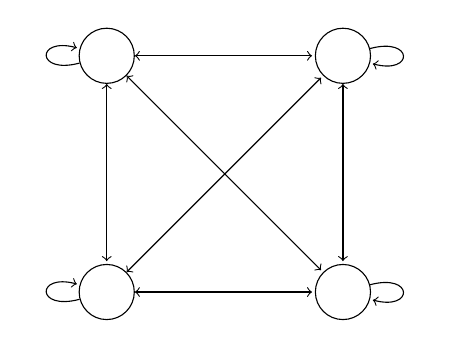
\begin{tikzpicture}[shorten >=1pt,<->,draw=black, node distance=\layersep]
	\tikzstyle{neuron}=[circle,draw=black,,minimum size=12pt,inner sep=0pt,text width=2em, text centered]    
	\node[neuron] (N-1) at (0,0) {};
	\node[neuron] (N-2) at (0,-3) {};
	\node[neuron] (N-3) at (3,0) {};
	\node[neuron] (N-4) at (3,-3) {};
	\path[] (N-1) edge [loop left] node {} (N-1);
	\path[] (N-2) edge [loop left] node {} (N-2);
	\path[] (N-3) edge [loop right] node {} (N-3);
	\path[] (N-4) edge [loop right] node {} (N-4);
         \path (N-1) edge (N-2);
         \path (N-1) edge (N-3);
         \path (N-1) edge (N-4);
          \path (N-2) edge (N-3);
          \path (N-2) edge (N-4);
          \path (N-3) edge (N-4);
\end{tikzpicture}
}
\newcommand{\partiallyconnected}[1][]{
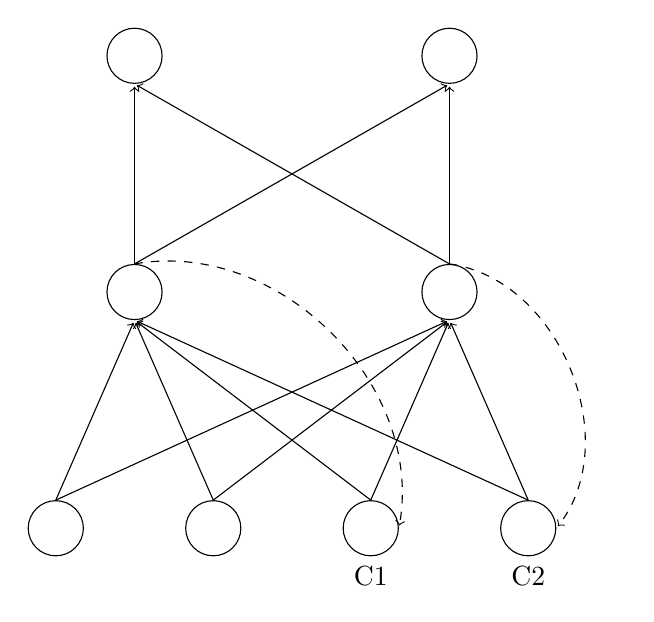
\begin{tikzpicture}[shorten >=1pt,->,draw=black, node distance=\layersep]
	\tikzstyle{neuron}=[circle,draw=black,,minimum size=12pt,inner sep=0pt,text width=2em, text centered]    
	\node[neuron] (O-1) at (0,0) {};
	\node[neuron] (O-2) at (-4,0) {};
	\node[neuron] (H-1) at (0,-3) {};
	\node[neuron] (H-2) at (-4,-3) {};
	\node[neuron, label=below:C1] (I-1) at (-1,-6) {};
	\node[neuron, label=below:C2]  (I-2) at (1,-6) {};
	\node[neuron]  (I-3) at (-3,-6) {};
	\node[neuron] (I-4) at (-5,-6) {};
	
	\foreach \source in {1,2}{
		 \foreach \dest in {1,2} {
           		\path (H-\source.north) edge (O-\dest.south);
			\path (I-\source.north) edge (H-\dest.south);
		}
	}
	\foreach \source in {3,4}{
		 \foreach \dest in {1,2} {
			\path (I-\source.north) edge (H-\dest.south);
		}
	}
	\path[dashed] (H-1.north) edge[bend left=60] (I-2.east);
	\path[dashed] (H-2.north) edge[bend left=55]  ($(I-1.east)$);
\end{tikzpicture}

}
% !TEX root = ../thesis.tex

\newcommand{\candidatestree}[1][]{% 1 optional parameter for options for the tikz picture
\begin{tikzpicture}[grow=right, ->,
  baseline,
  level distance=20mm,
  text depth=.1em,
  text height=.8em,
  level distance=80pt,
  level 1/.style={sibling distance=40em},
  level 2/.style={sibling distance=45em},
  level 3/.style={sibling distance=20em},
  level 4/.style={sibling distance=10em},
  level 5/.style={sibling distance=5em}]
\node {0000}
    child { node {done} edge from parent[solid] }
    child {
        node {1000}  edge from parent[dashed]     
        child {
		node {0100} edge from parent[solid]
		child { 
			node {0010} edge from parent[solid]
			child { 
				node {0001} edge from parent[snake]
				child { 
					node {done} edge from parent[snake] 
				}
			}
		}
		child {
			node {0010}
			edge from parent[dashed]
			child { 
				node {0001} edge from parent[solid]
				child { 
					node {done} edge from parent[solid] 
				}
				child { 
					node {0101} edge from parent[dashed]
					child { 
						node {done} edge from parent[solid,snake] 
					}
				}
			}
			child {
				node {0001} edge from parent[dashed]
				child {
					node {0110} edge from parent[solid]
					child { 
						node {done} edge from parent[solid,snake] 
					}
				}
				child { 
					node {0110} edge from parent[dashed]
					child { 
						node {0101} edge from parent[solid,snake]
						child { 
							node {done} edge from parent[solid,snake] 
						}
					}
				}
			}
		}
	}
	child {
                node {0100} edge from parent[dashed]
                	child {
			node {0010} edge from parent[solid]
			child {
				node {0001} edge from parent[solid]
				child { node {done} edge from parent[solid] }
				child { 
					node {1001} edge from parent[dashed]
					child { 
						node {done} edge from parent[solid,snake] 
					}
				}
			}
			child {
				node {0001} edge from parent[dashed]
				child {
					node {1010}
					edge from parent[solid]
					child { 
						node {done} edge from parent[solid,snake] 
					}
				}
				child {
					node {1010}
					edge from parent[dashed]
					child {
						node {1001} edge from parent[solid,snake]
						child { 
							node {done} edge from parent[solid,snake] 
						}
					}
				}
			}
		}
		child {
			node {0010} edge from parent[dashed]
			child {
				node {0001}
				edge from parent[solid]
				child {
					node {done}
					edge from parent[solid]
				}
				child {
					node {1001} edge from parent[dashed]
					child {
						node {0101} edge from parent[solid, snake]
						child {
							node {done} edge from parent[solid, snake]
						}
					}
				}
			}
			child {
				node {0001} edge from parent[dashed]
				child {
					node {1010} edge from parent[solid]
					child {
						node {0110} edge from parent[solid, snake]
						child { 
							node {done} edge from parent[solid,snake]
						}
					}
				}
				child {
					node {1010} edge from parent[dashed]
					child { 
						node {1001} edge from parent[solid, snake] 
						child {
							node {0110} edge from parent[solid,snake] 
							child { 
								node {0101} edge from parent[solid,snake] 
								child { 
									node {done} edge from parent[solid,snake]
								}
							}
						}
					}
				}
			}
		}
	}
    };
\end{tikzpicture}
}
% !TEX root = ../thesis.tex
% ------------------------------------------------------------------------------------------------------------------------------------------------------------ %
\newcommand{\coreoverview}[1][]{% 1 optional parameter for options for the tikz picture
\def\layersep{3cm}
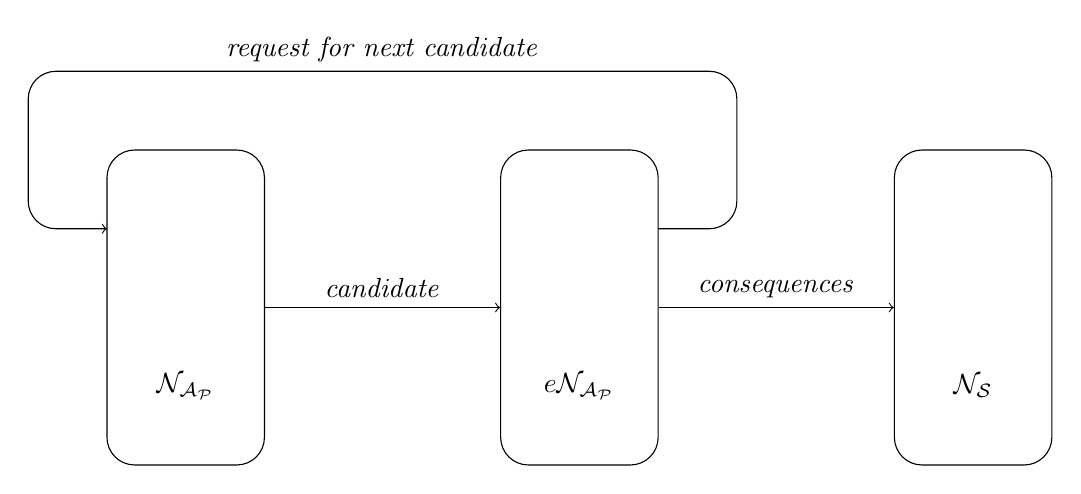
\begin{tikzpicture}

\draw (0,0) node [rectangle,draw=black,minimum height=4cm, minimum width=2cm, text centered, rounded corners = 10pt] (A) {};
\draw (0,-1) node [black, text centered] (C) {$\CalN_{\CalA_{\CalP}}$};
\draw (5,0) node [rectangle,draw=black,minimum height=4cm, minimum width=2cm, text centered,, rounded corners = 10pt] (P) {};
\draw (5,-1) node [black, text centered] (C) {$e\CalN_{\CalA_{\CalP}}$};
\draw (10,0) node [rectangle,draw=black,minimum height=4cm, minimum width=2cm, text centered,, rounded corners = 10pt] (S) {};
\draw (10,-1) node [black, text centered] (C) {$\CalN_\CalS$};

\draw [black,->] (A) -- node [above] {\textit{candidate}} (P);

\draw [->, black, rounded corners = 10pt]  (6,1) to (7,1) to (7, 3) to node [above] {\textit{request for next candidate}}  (-2,3) to (-2,1) to (-1,1);
\draw [black,->] (P) -- node [above] {\textit{consequences}} (S);
%\draw [->, black, rounded corners = 10pt]  (6,-1) to (7,-1) to (7, -3) to node [below] {whether candidate was positive} (-2,-3) to (-2,-1) to (-1,-1);

\end{tikzpicture}
} 
\hypersetup{					% setup the hyperref-package options
	pdftitle={\thesisTitle},	% 	- title (PDF meta)
	%pdfsubject={\thesisSubject},% 	- subject (PDF meta)
	pdfauthor={\thesisName},	% 	- author (PDF meta)
	plainpages=false,			% 	-
	colorlinks=false,			% 	- colorize links?
	pdfborder={0 0 0},			% 	-
	breaklinks=true,			% 	- allow line break inside links
	bookmarksnumbered=true,		%
	bookmarksopen=true			%
}
\newglossaryentry{d}
{
  name=$\top$,
  description={Truth value \textit{true}},
  sort={1}
}
\newglossaryentry{e}
{
  name=$\bot$,
  description={Truth value \textit{false}},
  sort={1}
}
\newglossaryentry{f}
{
  name=$\udf$,
  description={Truth value \textit{unknown}},
  sort={3}
}
\newglossaryentry{a}
{
  name=$\CalP$,
  description={Logic program},
  sort={4}
}
\newglossaryentry{b}
{
  name=$\Comp\CalP$,
  description={Completion of $\CalP$},
  sort={5}
}
\newglossaryentry{c}
{
  name=$\WComp\CalP$,
  description={Weak completion of $\CalP$},
  sort={6}
}
\newglossaryentry{g}
{
  name=$\Atoms(\CalP)$,
  description={Set of all atoms occurring in $\CalP$},
  sort={7}
}
\newglossaryentry{h}
{
  name=$\Def(\CalP)$,
  description={Set of all defined atoms occurring in $\CalP$},
  sort={8}
}
\newglossaryentry{i}
{
  name=$\Undef(\CalP)$,
  description={Set of all undefined atoms occurring in $\CalP$},
  sort={9}
}
\newglossaryentry{l}
{
  name=$\CalA_\CalP$,
  description={Set of abducibles for a program $\CalP$},
  sort={10}
}
\newglossaryentry{j}
{
  name=$\CalIC$,
  description={Set of integrity constraints},
  sort={11}
}
\newglossaryentry{m}
{
  name=$\CalO$,
  description={Observation},
  sort={12}
}
\newglossaryentry{n}
{
  name=$\CalE$,
  description={Explanation},
  sort={13}
}
\newglossaryentry{t}
{
  name=$\CalC$,
  description={Candidate explanation},
  sort={14}
}
\newglossaryentry{o}
{
  name=$\CalC_{\CalA_\CalP}$,
  description={Set of candidate explanations for the set of abducibles $\CalA_\CalP$},
  sort={15}
}
\newglossaryentry{q}
{
  name=$\models$,
  description={Consequence relation},
  sort={16}
}
\newglossaryentry{r}
{
  name=$\ModelsWCS$,
  description={Consequence relation under the weak completion semantics},
  sort={17}
}
\newglossaryentry{p}
{
  name=$\Lfp$,
  description={Least fixed point},
  sort={18}
}
\newglossaryentry{s}
{
  name=$\Phi_\CalP$,
  description={Semantic operator introduced by Stenning and van Lambalgen},
  sort={19}
}
\newglossaryentry{u}
{
  name=$\CalI$,
  description={Interpretation},
  sort={20}
}
\newglossaryentry{w}
{
  name=$\CalI^\top$,
  description={Interpretation consisting of the atoms that are mapped to $\top$},
  sort={21}
}
\newglossaryentry{x}
{
  name=$\CalI^\bot$,
  description={Interpretation consisting of the atoms that are mapped to $\bot$},
  sort={22}
}
\makeglossaries
\glsaddall
% **************************************************
% Document CONTENT
% **************************************************
\begin{document}

% --------------------------
% rename document parts
% --------------------------
%\renew
%\renewcaptionname{ngerman}{\figurename}{Abb.}
%\renewcaptionname{ngerman}{\tablename}{Tab.}
%\renewcaptionname{english}{\figurename}{Fig.}
%\renewcaptionname{english}{\tablename}{Tab.}
\newtheorem{prop}{Proposition}
\newtheorem{definition}{Definition}
\newtheorem{example}{Example}
\newtheorem{algorithm}{Algorithm}
% --------------------------
% Front matter
% --------------------------
\pagenumbering{roman}			% roman page numbing (invisible for empty page style)
\pagestyle{empty}				% no header or footers
% !TEX root = ../thesis.tex
% ------------------------------------  --> cover title page
\begin{titlepage}
	\pdfbookmark[0]{Cover}{Cover}
	\flushright
	\hfill
	\vfill
	{\LARGE\thesisTitle \par}
	\rule[5pt]{\textwidth}{.4pt} \par
	{\Large\thesisName}
	\vfill
	\textit{\large\thesisDate} \\
	%Version: \thesisVersion
\end{titlepage}


% ------------------------------------  --> main title page
\begin{titlepage}
	\pdfbookmark[0]{Titlepage}{Titlepage}
	\tgherosfont
	\centering

	{\Large \thesisUniversity} \\[4mm]
	
\includegraphics[width=6cm]{figures/logo_tud} \\[2mm]
	\textsf{\thesisUniversityDepartment} \\
	\textsf{\thesisUniversityInstitute} \\
	\textsf{\thesisUniversityGroup} \\

	\vfill
	%{\large \thesisSubject} \\[5mm]
	{\LARGE \color{ctcolortitle}\textbf{\thesisTitle} \\[10mm]}
	{\Large \thesisName} \\

	\vfill
	\begin{minipage}[t]{.27\textwidth}
		\raggedleft
		\textit{1. Reviewer}
	\end{minipage}
	\hspace*{15pt}
	\begin{minipage}[t]{.65\textwidth}
		{\Large \thesisFirstReviewer} \\
	  	{\small \thesisFirstReviewerDepartment} \\[-1mm]
		{\small \thesisFirstReviewerUniversity}
	\end{minipage} \\[5mm]
	\begin{minipage}[t]{.27\textwidth}
		\raggedleft
		\textit{2. Reviewer}
	\end{minipage}
	\hspace*{15pt}
	\begin{minipage}[t]{.65\textwidth}
		{\Large \thesisSecondReviewer} \\
	  	{\small \thesisSecondReviewerDepartment} \\[-1mm]
		{\small \thesisSecondReviewerUniversity}
	\end{minipage} \\[10mm]
	\begin{minipage}[t]{.27\textwidth}
		\raggedleft
		\textit{Supervisor}
	\end{minipage}
	\hspace*{15pt}
	\begin{minipage}[t]{.65\textwidth}
		\thesisFirstSupervisor
	\end{minipage} \\[10mm]

	\thesisDate \\

\end{titlepage}


% ------------------------------------  --> lower title back for single page layout
\hfill
\vfill
{
	\small
	\textbf{\thesisName} \\
	\textit{\thesisTitle} \\
	%\thesisSubject, 
	\thesisDate \\
	Reviewers: \thesisFirstReviewer\ and \thesisSecondReviewer \\
	Supervisor: \thesisFirstSupervisor \\[1.5em]
	\textbf{\thesisUniversity} \\
	\textit{\thesisUniversityGroup} \\
	\thesisUniversityInstitute \\
	\thesisUniversityDepartment \\
	\thesisUniversityStreetAddress \\
	\thesisUniversityPostalCode\ and \thesisUniversityCity
}		% INCLUDE: all titlepages
\cleardoublepage

\pagestyle{plain}				% display just page numbers
% !TEX root = ../thesis.tex

\pdfbookmark[0]{Abstract}{Abstract}
\chapter*{Abstract}
\label{sec:abstract}

Well known psychological experiments have shown that classical logic does not seem to be adequate for modelling human reasoning. Therefore, we focus on an approach called the weak completion semantics which considers the least model of the weak completion of logic programs under the three-valued {\L}ukasiewicz logic. This approach has shown how to adequately model many of the famous human reasoning tasks found in the literature, mostly by means of sceptical abduction. The reasoning is done by searching for all the abductive explanations for a given observation and computing which consequences can be derived from them. 

The computation of sceptical consequences for an abductive problem has been encoded by means of a connectionist network. Abduction is known to be a computationally expensive problem, where computing the abductive sceptical consequences is DP-complete. The bottleneck of this problem is in the exponential number of candidate explanations that have to be considered. Therefore, we focus on the component of the connectionist network responsible for generating those candidates and try to optimise it.

We start by adding a minimality constraint to the generation of candidate explanations, which considerably reduces the number of candidates generated in practice, but the problem still remains the same in the worst case. We assume that humans do not consider all the candidate explanations when reasoning about skeptical abduction, but rather a subset of them. Therefore, we propose to substitute the current approach by a recurrent network such as Jordan or Elman networks which we have shown to be capable of learning arbitrary sequences of candidate explanations.

It is commonly required from computational models in artificial intelligence to exhibit a behaviour similar to the biological brain. Therefore, we propose some psychological experiments to confirm the assumptions we have made, bearing in mind that our approach has been designed in such a way that it could easily be aligned with these psychological experiments independent of their outcome.		% INCLUDE: the abstracts (english and german)
\cleardoublepage
%
%% !TEX root = ../thesis.tex

\pdfbookmark[0]{Acknowledgement}{Acknowledgement}
\chapter*{Acknowledgement}
\label{sec:acknowledgement}
\vspace*{-10mm} % INCLUDE: acknowledgement
\cleardoublepage
%
\setcounter{tocdepth}{2}		% define depth of toc
\tableofcontents			% display table of contents
\cleardoublepage

% --------------------------
% Body matter
% --------------------------
\pagenumbering{arabic}		% arabic page numbering
\setcounter{page}{1}			% set page counter
\pagestyle{maincontentstyle} 	% fancy header and footer

% !TEX root = ../thesis.tex

\chapter{Introduction}
\label{sec:intro}

Many human reasoning tasks have been adequately modelled by a computational approach based on the weak completion semantics. In most of the cases, the models generated by this approach rely on the sceptical abductive consequences of an observation and the least model of a logic program representing the given background knowledge. This approach has been encoded as a connectionist network which is going to be the focus of this thesis. In this chapter, we show some of the mentioned reasoning problems as well as an overview of this network's architecture. 

\section{Sceptical Abduction}

The notion of abduction was first introduced by the philosopher Pierce \cite{quine1933collected}. Let us illustrate the idea of abduction by means of an example. Consider a background knowledge consisting of the following conditionals:
\[
\begin{array}{l}
\mbox{\textit{If it rained last night, then the grass is wet.}}\\
\mbox{\textit{If the sprinkler was on, then the grass is wet.}}\\
\mbox{\textit{If the grass is wet, then the shoes are wet.}}\\
\end{array}
\]
If we observe that the shoes are wet, we have several explanations. One explanation is that the grass is wet. However, we can further explain, why the grass is wet. Then, we obtain the explanation \textit{it rained last night} and the explanation \textit{the sprinkler was on}. The last two explanations are called basic, since we cannot further explain them. Another explanation is \textit{the sprinkler was on and it rained last night}, which combines the last two explanations. Then, this explanation is not minimal. One meaningless explanation is \textit{the shoes are wet}, i.e. the observation is explained by itself.

There are two forms of abduction which are well known in the literature: credulous and sceptical abduction. In credulous abduction, considering a specific background knowledge, humans would derive a conclusion if it follows from at least one of the explanations for the given observation. On the other hand, this is not sufficient in sceptical abduction where all explanations shall be considered. Coming back to the example, if we observe that \textit{the grass is wet}, then we could credulously conclude that \textit{it rained last night}. However, in the scenario where \textit{the sprinkler was on}, our observation is also explained and not necessarily \textit{it rained last night} has to be true. Therefore, we can neither sceptically conclude that \textit{it rained last night} nor that \textit{the sprinkler was on}.

As we will discuss in more details later on, psychological experiments have shown that humans systematically deviate from the classical logically correct answers. Therefore, we will consider a non-classical approach to model human reasoning which is non-monotonic and based on the least model of the weak completion of logic programs. More precisely, here we focus focus on the component of this framework responsible for deciding which and in what order possible explanations should be considered.

\subsection{Byrne's Suppression Task}

A well-known psychological experiment by Byrne \cite{byrne1989suppressing} has shown that, in certain circumstances, participants reject instances of the valid \textit{modus ponens} and \textit{modus tollens} inference form in conditional arguments. This experiment shows that people might suppress previously drawn conclusions when additional information becomes available. For example, when a conditional premise, such as \textit{if she has an essay to finish, then she will study late in the library} is accompanied by the fact \textit{she has an essay to finish}, 96\% of the participants conclude that \textit{she will study late in the library}. However, if we add the conditional premise \textit{if the library stays open, she will study late in the library}, then the number of participants which conclude that \textit{she will study late in the library} drops to 38\%.

This experiment is a strong support for the assumption that humans reason non-monotonically. In the complete experiment, participants receive the following three conditionals:
\[
\begin{array}{ll}
\mbox{\textbf{Simple}} & \mbox{\textit{If she has an essay to finish, then she will study late in the library}}.\\
\mbox{\textbf{Alternative}} & \mbox{\textit{If she has a textbook to read, then she will study late in the library}}.\\
\mbox{\textbf{Additional}} & \mbox{\textit{If the library stays open, then she will study late in the library}}.
\end{array}
\]

The participants were divided into three groups such that each group received a different combination of these conditionals:
\[
\begin{array}{ll}
\mbox{\textbf{Group I}} & \mbox{Simple}.\\
\mbox{\textbf{Group II}} & \mbox{Simple + Alternative}.\\
\mbox{\textbf{Group III}} & \mbox{Simple + Additional}.
\end{array}
\]

The task given to the participants consisted of two parts. In the first part the participants got either the fact \textit{she has an essay to finish} ($e^\top$) or the negation of it, \textit{she does not have an essay to finish} ($e^\bot$). In the second part the participants got either the fact \textit{she will study late in the library} ($l^\top$) or the negation of it, \textit{she will not study late in the library} ($l^\bot$). Based on the given information, the participants were asked to draw conclusions.

\begin{table}
\centering
\begin{tabular}{ccccc}
Fact & Conclusion & Group I & Group II & Group III\\
\hline
\hfill	\\		
$e^\top$ & $l^\top$ & 96\% & 96\% & \textbf{38\%}\\
$e^\bot$ & $l^\bot$ & 46\% & \textbf{4\%}   & 63\%\\
$l^\top$ & $e^\top$ & 53\% & \textbf{16\%} & 55\%\\
$l^\bot$ & $e^\bot$ & 69\%  & 69\% & \textbf{44\%}
\end{tabular}
\bigskip
\caption{Empirical results about suppression obtained by Byrne.}
\label{table:suppresion}
\end{table}

An overview of the empirical results obtained from this experiment is shown in Table~\ref{table:suppresion}. Percentages indicate the proportion of participants in each of the three groups that have drawn the respective conclusion from the indicated given fact and the conditionals. Where suppression took effect, the propositions are highlighted in bold. Similar results have been obtained by other researchers, see for example~\cite{dieussaert2000strategies}.

The suppression task is adequately modelled by the weak completion semantics using skeptical abduction. In particular, consider the case where we observe that \textit{she will study late in the library} is true. If we model only the conditional given to Group I, the consequence that \textit{she has an essay to finish} is derived, while if we model the conditionals given to Group II, this is no longer the case. If we observe the psychological results, our approach is able to suppress the conclusion when one more conditional to the background knowledge is added, reflecting the answers given by the participants.

\subsection{Wason's Selection Task}

In the original selection task \cite{wason1968reasoning} participants were told that each card had a letter on one side of the card and a number on the other side of the card. They were presented the following four cards the table:
\[
\framebox(50,55){D}  \quad\quad\quad \framebox(50,55){F}  \quad\quad\quad
\framebox(50,55){3}  \quad\quad\quad \framebox(50,55){7} 
\]
The task of the participants was to evaluate the following conditional with respect to each of the four cards:
\[
\mbox{\textit{if there is a D on one side of the card, then there is 3 on the other side.}}
\]
Which cards must be turned over in order to find out whether the conditional holds?

Assume the conditional is represented in classical propositional logic by the implication 
\[
3 \leftarrow D
\]
where the propositional variable \textit{3} represents the fact that the number 3 is shown and \textit{D} represents the fact that the letter D is shown. Then, in order to verify  the implication one must turn the cards showing D and 7. However, as repeated experiments have shown consistently (see Table~\ref{table:abstract}), participants believe differently. 

Whereas 89\% of the participants correctly determine that the card showing D must be turned (a number other than 3 on the other side would falsify the implication), 62\% of the participants incorrectly suggests turning the card showing 3 (no relevant information can be found which would falsify the implication). Likewise, whereas only 25\% of the participants correctly believe that the card showing 7 need to be turned (if the other side would show a D, then the implication is falsified), 16\% incorrectly believe that the card showing F needs to be turned (no relevant information can be found which would falsify the implication). In other words, the overall correctness of the answers for the abstract selection task if modelled by an implication in classical two-valued logic is pretty bad.

The selection task was adapted to a social case \cite{griggs1982elusive}. Consider the following four cards:
\[
\framebox(50,55){beer}  \quad\quad\quad \framebox(50,55){coke}  \quad\quad\quad 
\framebox(50,55){22 years} \quad\quad\quad  \framebox(50,55){16 years} 
\]

Each card has the person's age on one side of the card and what the person is drinking on the other side of the card. Consider the conditional
\[
\mbox{\textit{if a person is drinking beer, then the person must be over 19 years of age.}}
\]
The same question is then asked: Which cards must be turned over in order to find out whether the conditional holds?

If the conditional is represented by the implication 
\[
over19 \leftarrow beer,
\]
where $over19$ represents a person being older than 19 years and \textit{beer} represents the person drinking beer. In order to verify the implication, one must turn the cards drinking beer and 16 years old. Participants usually solve the social version of the selection task classical logically correctly. Table~\ref{table:social} shows the results represented by Griggs and Cox \cite{cox1982effects} for the social case. 

\begin{table}
	\centering
	\begin{subtable}[h]{0.30\textwidth}
		\begin{tabular}{cccc}
			D & F & 3 & 7 \\
			\hline
			89\% & 16\% & 62\% & 25\%
		\end{tabular}
		\bigskip
		\caption{Abstract case.}
		\label{table:abstract}
	\end{subtable}
	\hspace{2cm}
	\begin{subtable}[h]{0.30\textwidth}
		\begin{tabular}{cccc}
			beer & coke & 22yrs& 16yrs\\
			\hline
			95\% & 0.025\% & 0.025\% & 80\%
		\end{tabular}
		\bigskip
		\caption{Social case.}
		\label{table:social}
	\end{subtable}
	\hspace{1cm}
	\bigskip
	\caption{The results of the abstract (a) and social (b) cases of the selection task.}
\end{table}

One explanation for the differences between both cases can be found in \cite{kowalski2011computational}, namely that people view the conditional in the abstract case as a belief. For instance, the participants perceive the task to examine whether the rule is either \textit{true} or \textit{false}. On the other hand, in the social case, the participants perceive the rule as a social constraint, a conditional that ought to be \textit{true}. People intuitively aim at preventing the violation of such a constraint, which is normally done by observing whether the state of the world complies with the rule.

Both abstract and social cases can be modelled by an approach based on the weak completion semantics shown in \cite{dietz2013computational}. The fact that two conditionals following the same syntactic structure were evaluated differently gives a strong intuition that the semantics is also an important criteria to be considered when modelling those reasoning tasks. In the next section the discussion on the semantics of conditionals is developed in more details.

\subsection{Conditionals Semantics}

Conditionals can be categorised in many different types and classes, but there are two main groups of conditionals: indicative and subjunctive conditionals, the latter of which are also known as counterfactuals. In indicative conditionals both, the condition and the consequence, can be either true, false or unknown. But if the condition is true, then the consequence is asserted to be true. In counterfactuals, the consequence can again be either true, false or unknown, but the condition is known to be false. Besides that, in the couterfactual circumstance of the condition being true, the consequence is asserted to be true.

In we focus on indicative conditionals, there are many subclasses to be considered. For example, they can be classified into \textit{obligation} and \textit{factual conditionals}. The difference between them is that in the \textit{obligation conditionals} the consequence is obligatory, while in the \textit{factual conditionals} this is not  the case. More precisely, given an \textit{obligation conditionals} it can never be the case that the condition happens and the consequence doesn't.

As explained in \cite{byrne2007rational}, conditionals where the consequent is denied are more likely to be evaluated to \textit{true} if it is an \textit{obligation conditional}. This happens because for this type of conditionals, people keep in mind a forbidden possibility where condition and not consequence happens together and, in this case, if not consequence is  known to be \textit{true}, then it cannot be the case that condition is \textit{true} as well, otherwise the forbidden possibility is violated. Thus, \textit{not condition} is concluded.  But, since in a \textit{factual conditional} this forbidden possibility does not exist, conditionals with the consequence denied should be evaluated to \textit{unknown}. 

Consider the following conditional:
\[
\begin{array}{c}
\mbox{\textit{If it rains, then the streets are wet.}}
\end{array}
\]
Its consequence is obligatory. We cannot easily imagine a case where the condition the \textit{it rains} is true and the consequence \textit{the streets are wet} is not. We know streets, we know rain and its effects, and because the conditional is discussed without any specific context, there does not appear to be a case where the condition is true and the consequence is not. But if we now consider the following conditional:
\[
\begin{array}{c}
\mbox{\textit{If it rains, then she takes her umbrella.}}
\end{array}
\]
Is consequence is not obligatory. Different than in the previous case, is the condition \textit{it rains} is true, we can easily think about a scenario where the consequence \textit{she takes her umbrella} is not. It is not so counterintuitive to imagine that it rained and she forgot to take her umbrella, for example.

In the selection task, the conditional considered in the abstract case is classified as a \textit{factual conditional} as there is no obligation implied from the context. On the other hand, the conditional considered in the social case is classified as an \textit{obligation conditional} as there is a clear obligation implied from the \textit{must} condition. There are also semantic differences in the conditions of these conditionals which are discussed in \cite{saldanhaobligation}.

\subsection{Syllogistic Reasoning}

A syllogism consists of two premises and a conclusion. Each of them is a quantified statement using one of the four quantifiers \textit{all}, \textit{no}, \textit{some}, and \textit{some are not} over sets of entities which we denote in the following by a, b, and c. An example of a syllogism is:
\[
\begin{array}{l}
\mbox{\textit{Some b are a}}\\
\mbox{\textit{No b are c}}
\end{array}
\]

In experiments, participants are normally expected to complete the syllogism by drawing a logical consequence from the first two premises, e.g. in this example \textit{some a are not c}. Altogether, there are 64 syllogisms and, if formalised in first-order logic, we can compute their logical consequence in classical logic. The first two premises together with a consequence that follows classical logically is called a \textit{valid syllogism}. Otherwise, it is called an \textit{invalid syllogism}.

A meta-analysis by Khemlani and Johnson Laird \cite{khemlani2012theories} based on six experiments has shown that humans do not only deviate from the classical predictions of first-order logic, but from any other of at least twelve cognitive theories on the syllogistic reasoning. To understand the deviation from classical logic on the experimental results, let us consider an example of a syllogism discussed by Evans \cite{evans2013reasoning} which has an invalid but believable conclusion as well as a valid but unbelievable conclusion. Given the following two premises:
\[
\begin{array}{l}
\mbox{\textit{No addictive things are inexpensive.}}\\
\mbox{\textit{Some cigarettes are inexpensive.}}
\end{array}
\]
The conclusion that \textit{some addictive things are inexpensive} is invalid, but believable. On the other hand, the conclusion that \textit{some cigarettes are not addictive} is valid, but unbelievable.

From the cognitive theories available in the literature, the best overall results are achieved by Polk and Newell, the Verbal Models Theory \cite{polk1995deduction}, which predicts 84\% of the participants responses, closely followed by Johnson-Laird, the Mental Model Theory \cite{johnson1983mental}, with 83\%, whereas PSYCOP \cite{rips1994psychology} by Rips only predicts 77\% of the participants' responses. 

Recently, a new cognitive theory, based on the weak completion semantics and skeptical abduction, to model the syllogistic reasoning task has been developed by Costa, Dietz, H{\"o}lldobler and Ragni \cite{da2017computational}. This approach identifies seven principles, mostly motivated from findings in cognitive science, which are necessary to draw the inferences. This approach has achieved the best results, compared to the results of other cognitive theories, with a prediction of 89\%.

\section{A Core Method for Sceptical Abduction}

H{\"o}lldobler and Kencana Ramli \cite{holldobler2009logics} have shown that the computation of the least fixed point of the $\Phi_\CalP$ operator can be realised within a connectionist network, with the core-method \cite{bader2006core}. A connectionist realisation of sceptical abduction under the weak completion semantics within the core method has been showed by Dietz Saldanha, H{\"o}lldobler, Kencana Ramli, and Palacios Medinacelli \cite{corepaper}. Figure~\ref{fig:coreoverview} shows an overview of this connectionist network which consists of three main components.

\begin{figure}[h]
\begin{center}
\scalebox{0.9}{\coreoverview}
\end{center}
\caption{Overall view of the connectionist network to compute the sceptical consequences of a given abductive problem.}
\label{fig:coreoverview}
\end{figure}

The first component of the network $\CalN_{\CalA_\CalP}$ sequentially generates the candidate explanations to be considered by the abductive framework one after the other and only upon request. The second component $e\CalN_{\CalA_\CalP}$ computes the least model of the weak completion of $\CalP \cup \CalC$, where $\CalP$ is the program considered as background knowledge and $\CalC$ is the current candidate explanation generated by $\CalN_{\CalA_\CalP}$. The network $e\CalN_{\CalA_\CalP}$ sends the request of a new candidate to network $\CalN_{\CalA_\CalP}$ once its task is done.

Besides the next candidate explanation, the network $\CalN_{\CalA_\CalP}$ also outputs the information whether the candidate generated is the last one. When that's the case, after the computation of the least model of this last candidate to be considered, the network $\CalN_\CalS$ computes all the sceptical consequences of the given observation by merging all the consequences followed by the program and the positive candidates.

The complexity of the task corresponding to component $\CalN_{\CalA_\CalP}$ is exponential with respect to the cardinality of the set of abducibles. The computation of the least fixed point of $\Phi_\CalP$, corresponding to component $e\CalN_{\CalA_\CalP}$, can be done in polynomial time as shown by Dietz Saldanha, H{\"o}lldobler, and Philipp \cite{saldanha1872contextual}. The remaining component, denoted by $\CalN_\CalS$, has the task of computing the sceptical consequences, given the consequences of each positive candidate. This can be done by intersecting the given consequences, which can be reduced to the problem of sets intersection. Therefore, it can also be done in polynomial time.

Based on the complexity of each of those tasks, it is clear that the bottleneck of the problem is in the generation of candidate explanations. This component is encoded by means of a McCulloch Pitts network designed to generate all the non-complementary candidate explanations in a static and pre-defined order. The complexity results of the way we apply sceptical abduction is a strong indication that humans do not reason in the same way. 

Motivated by this, we believe that humans do not generate all candidate explanation but rather a subset of them. Therefore, we are going to make some assumptions in the reasoning process which will allow us to reduce the number of generated candidate explanations. However, as there are so many open questions regarding this problem which have not yet been verified, we also propose to substitute the current approach by a more flexible one which is able to learn arbitrary sequences of candidate explanations and, therefore, can easily be adapted to the constraints later identified in psychological experiments.

\section{Hypotheses}

In order to optimise the process of generating candidate explanations and align it with the real cognitive process regarding sceptical abduction, we are going to make some assumptions as, for example, regarding minimal and bounded candidates. In this section we will discuss these hypotheses and their implications in more details.

\subsection{Basic Candidate Explanations}

Reconsidering the first example presented in Section~1.1, the only possible explanations which would be considered in our approach for the observation \textit{the shoes are wet} are concerning that \textit{it rained last night} or that \textit{the sprinkler was on}, but not that the \textit{the grass is wet}. This is a consequence of the abductive framework where we only consider the undefined atoms in the set of abducibles which are later going to be used for the generation of candidate explanations. 

Therefore, our first hypothesis is that when humans reason about the sceptical consequences of a given problem they search for the basic candidate explanations and reason only with respect to them. An explanation is said to be basic if it cannot be explained by other facts or assumptions, i.e. it can only be explained by itself.

\subsection{Sequential Generation}

The second hypothesis we make is that humans do not generate several candidate explanations in parallel but they are sequentially generated and considered one by one in the reasoning process. Therefore, we do not have a distributed approach. Instead, the candidate explanations are generated after the other. Besides, a new candidate is generated only after our approach checks whether the current candidate is indeed an explanation for the given observation.

\subsection{Non-complementary Candidate Explanations}

Consider the following conditional: 
\[
\begin{array}{l}
\mbox{\textit{If she studies, then she will pass the exam.}}\\
\end{array}
\]
To explain, for instance, the observation that \textit{she did not pass the exam}, we would not consider as candidate explanation the facts that \textit{she studied} and that \textit{she did not study} together. This type of candidate explanations are said to be complementary. Therefore, in our approach we also have the hypothesis that humans only consider non-complementary candidate explanations.

\subsection{Minimal Candidate Explanations}

Another hypothesis is that humans generate only minimal candidate explanations. If we reconsider Byrne's selection task presented earlier, for the observation that \textit{she studies late in the library}, the minimal explanations would be either that \textit{she has an essay to finish} or that \textit{she has a text book to read}. The case where both explanations are combined also explains the given observation, but in a non-minimal way and, therefore, should not be considered. Moreover, the cases where \textit{she has an essay to finish} but \textit{she does not have a text book to read} and the other way around are also non-minimal explanations for the observation.

This hypothesis implies a constraint in the generation of the candidate explanations which is about the cardinality of the candidates. It is easy to see that if the candidate where \textit{she has an essay to finish} and \textit{she has a text book to read} are both true is generated before a candidate where only one of these two facts is true and the other one is unknown, then there is no way to avoid this non-minimal candidate as it's subset is not known yet. Given this observation, we assume the generation of candidates has to be done from the smaller to the larger sets of candidates, where smaller and bigger is defined by their cardinality. 

\subsection{Bounded Sceptical Abduction}

Although the minimality constraint reduces the number of candidate explanations generated in average, the complexity of the problem remains the same in the worse case. Imagine a ordering respecting the cardinality where the explanation \textit{she does not have an essay to finish} and \textit{she does not have a text book to read} is the last one. If we observe that \textit{she does not study late in the library}, the only possible explanation for our observation would be the last one, which means that all the candidates would have to be generated just as before.

As mentioned before, it is hard to believe that humans would systematically generate all the candidate explanation to solve such a problem. Therefore, we have the hypothesis that there is a bound in the generation of candidate explanation and that the reasoning process is different for different types of conditionals as it has been investigated in \cite{saldanhaobligation}. This implies that arbitrary sequences of candidate explanations have to be considered.

\section{Tasks}

Considering the hypotheses we have made, we will now show what has to be done in the current approach to achieve such results. The tasks consist of two steps: first, we will show how to apply the minimality characterisation to the current McCulloch Pitts network, and, after this, we show a formal specification on how to substitute this component by a recurrent network which can learn arbitrary sequences of candidates.

\subsection{Minimality}

Given that the McCulloch Pitts network generates the candidate explanations in a static and pre-defined order, we can easily consider a sequence which respects the cardinality ordering. Given that the candidates are being generated from the smaller to the larger ones, we can store the information of which candidates were positive and use this information to block the generation of further candidates which are supersets of them. 

This can be done by adding a unit to the network corresponding to each of the candidates with cardinality larger than one. These units will be connected to all the units representing subsets of the respective candidate such that they are activated as soon as one of these candidates has been detected as being an explanation. The activation of these units will be stored for the further time steps and used later on to skip the generation of the non-minimal candidates. By this thechnique we ensure that only minimal candidate explanations are generated.

\subsection{Arbitrary Sequences}

In order to confirm our hypothesis on the bounded candidates and try to obtain more properties in the arbitrary sequence of candidates, we design some psychological experiments and propose their execution. Considering that there are so many open questions concerning this problem and that the psychological results are crucial to obtain a strong cognitive theory, we propose the substitution of the current approach by a recurrent network which can learn arbitrary sequences of candidate explanations and, therefore, easily adapt to the outcome of these experiments independent on what they are.

For this purpose, we will focus on Jordan and Elman networks and provide a formal specification on how they can be constructed, trained and tested for the problem of generating candidate explanations. This process evolves transforming our problem in a temporal domain problem and generating data which simulates the candidate explanations expected in different scenarios. We will start by showing that they can achieve the same results presented by the previous approach, but with the advantage of learning arbitrary sequences. We will design experiments to define the necessary number of hidden units such that they perform the task with a error rate close to~zero.

\section{Contributions}

\textbf{Optimisation of sceptical reasoning}

Sceptical abductive reasoning is an expensive problem from the computational point of view and its bottleneck is the exponential number of candidate explanations which has to be considered. By introducing the minimality constraint, we have reduced the number of candidate explanations generated in the average case, optimising with this the abductive sceptical reasoning process as a whole.

\textbf{Flexibility}

The current framework to generate candidate explanations is a McCulloch Pitts network which is designed to generated the candidate explanations as a static and pre-defined sequence. The replacement of this framework by a recurrent network which is able to learn arbitrary sequences of candidate explanations have given flexibility to our framework. As the sceptical reasoning approach is currently done based on several hypotheses which have not yet been tested, flexibility is crucial characteristic. 

\textbf{Bounded reasoning}

From a cognitive aspect, it is hard to believe that humans generate this large number of candidate explanations in the reasoning process. We believe that they rather generate a subset of these candidate explanations. By introducing the minimality constraint, we have considerably reduced the number of candidate explanations generated in the average case. However, the problem remains the same in the worst case. Moreover, there is still a considerably large number of candidates even after applying minimality. 

Based on this, we believe that a bound is applied when generating candidate explanations and, therefore, we have introduce this feature to our framework. As the network has an anytime behaviour, it remains only to defined what kind of bounds are applied and their characterisation. For this purpose, we need psychological experiments which are beyond the scope of this master thesis. However, the approach in designed in such a way which that it can easily be adapted to the experiments outcome.  

\textbf{Cognitive adequacy}

Throughout the development of this new approach, we have made several hypotheses which raises questions to be answered by means of psychological experiments. These questions have been discussed and an initial setup for experiments to test them has been proposed. Some of the hypotheses make sense from a computational point of view, but as we also want our approach to be cognitively adequate, carrying out these experiments is a crucial step. 

\section{Thesis Structure}

Although we assume the reader to be familiar with logic, logic programming and connectionist networks, Chapter~\ref{sec:preliminaries} introduces some of the general and basic concepts necessary as background knowledge for the work developed. The chapter is divided in two main parts: abduction under the weak completion semantics and connectionist networks. For the first part, we start by introducing some concepts on logic programs such as the weak completion, then we define which semantics we are going to consider throughout the thesis and finally de define the abductive framework as well as its complexity. For the second part, we start by introducing some general concepts of recurrent networks and focus then on Jordan and Elman networks which are going to be used later on.

In Chapter~\ref{sec:cn} we describe an approach based on McCulloch Pitts networks to generate non-complementary candidate explanations for the abductive problem. Later we introduce a possible extension of this approach such that it will now only generate minimal candidates. All the steps necessary for such modification are described by means of an example, but the algorithms on how to generalise to arbitrary problems is also presented.

After introducing the current approach for the generation of candidate explanations, in Chapter~\ref{sec:nn} we propose a new approach which is more flexible. We show that this approach can simulate the same behaviour as the previous one, with the advantage of learning arbitrary sequences of candidates. This is an important feature since we currently make assumptions on the process, but have not yet verified them by means of psychological experiments.

Finally, we want to evaluate the assumptions we have made and, as we already mentioned, a system that aims at being cognitively adequate has to be evaluated with respect to the way humans reason. Therefore, in Chapter~\ref{sec:exp} we suggest to carry out some psychological experiments. From their outcome, we expect to confirm or refute our hypothesis and extract more properties which can further improve our approach. 

 % INCLUDE: introduction
% !TEX root = ../thesis.tex

\chapter{Preliminaries}
\label{sec:preliminaries}

This chapter introduces the general notions and terminologies that will be used throughout this thesis, which are based on \cite{holldobler2009logic, lloyd2012foundations}. We start with Section~\ref{sec:preliminaries:abduction} by introducing some of the basic concepts about logic programming, the three-valued semantics and the weak completion semantics which are necessary to understand the abductive framework. Then in Section~\ref{sec:preliminaries:cn} we introduce some of the basic concepts about connectionist networks and recurrent connectionist networks which are going to be used later for the generation of candidate explanations for the abductive framework. In particular, we will introduce the architecture and main concepts of Jordan and Elman networks.

\section{Abduction under the Weak Completion Semantics}
\label{sec:preliminaries:abduction}

We assume the reader to be familiar with logic and logic programming. In the sequel, we will only consider propositional programs. If a program $\CalP$ is not propositional, then a propositional program $\CalP'$ corresponding to $\CalP$ can be obtained by grounding the program $\CalP$. We assume that each non-propositional program contains at least one constant symbol. The language $\CalL$ underlying a non-propositional program $\CalP$ contains precisely the predicate and constant symbols occurring in $\CalP$, and no others. Therefore, the following definitions can also be applied to programs which are not propositional. In those cases, we only need to compute the respective grounded program beforehand and reason with respect to it.

Therefore, we consider an \textit{alphabet} that consists of finite disjoint sets of \textit{propositional variables}, the \textit{truth-value constants true} $\top$, \textit{false} $\bot$ and \textit{unknown} $\udf$, and the usual connectives \textit{negation} $\neg$, \textit{disjunction} $\vee$, \textit{conjunction} $\wedge$, \textit{implication} $\leftarrow$, \textit{equivalence} $\leftrightarrow$. \textit{Formulas} are constructed in the usual way from the propositional variables, the truth-value constants and the connectives. An atomic formula is called an \textit{atom}. If~A is an atom, then $A$ and $\neg A$ are literals, called the \textit{positive literal} and the \textit{negative literal}, respectively. A \textit{language} $\CalL$ given by an alphabet $\CalA$ consists of the set of all formulas constructed from the symbols of $\CalA$.
 
\subsection{Logic Programs}
\label{sec:preliminaries:lp}

\begin{definition}
\label{def:clause}
\normalfont A \textit{clause} is a formula of the form:
\begin{align}
\label{rule:general} A \quad\leftarrow&\quad L_1 \wedge ... \wedge L_n.\\
\label{rule:fact} A \quad\leftarrow&\quad \top.\\
\label{rule:assumption} A \quad\leftarrow&\quad \bot.
\end{align}
A is called \textit{head} of the clause and the sub-formula to the right of the implication symbol is called \textit{body} of the clause. Clauses are also called \textit{rules} (\ref{rule:general}), \textit{facts} (\ref{rule:fact}) and \textit{assumptions} (\ref{rule:assumption}).

A given pair of clauses is said to be \textit{complementary} if they are of the following form
\[
\begin{array}{ccccccc}
c &\leftarrow& \top. &\quad& c &\leftarrow& \bot. 
\end{array}
\]
A set of clauses $\CalC$ is said to be \textit{complementary} if it contains a complementary pair; otherwise, $\CalC$ is said to be \textit{non-complementary}.
\end{definition}

\begin{definition}
\label{def:program}
\normalfont 
A \textit{logic program} $\CalP$ is a finite set of clauses. A \textit{propositional program} is a program where all clauses are propositional.
 
If $\CalP$ is a program, then $\Atoms(\CalP)$ denotes the set of all atoms occurring in $\CalP$. An atom $A$ is \textit{defined} in $\CalP$ if and only if $\CalP$ contains a clause of the form
\[
\begin{array}{lcl}
A &\leftarrow &Body. 
\end{array}
\]
$A$ is \textit{undefined in $\CalP$} if and only if $A$ is not defined in $\CalP$. The set of all atoms that are defined in $\CalP$ is denoted by $\Def(\CalP)$. The set of all atoms that are undefined in $\CalP$, that is $\Atoms(\CalP) \setminus \Def(\CalP)$, is denoted by $\Undef(\CalP)$. The \textit{definition} of $A$ in $\CalP$ is given by
\[
\begin{array}{c}
\Def(A, \CalP) =  \{ A \leftarrow Body \mid  A \leftarrow Body \mbox{ is a clause in } \CalP\}.
\end{array}
\]
\end{definition}

A \textit{normal program} \textendash\ in the standard sense used in the literature on logic programming \textendash\ is a program that does not contain assumptions. This means a program which consists only of rules and facts. The notion of assumptions, i.e., clauses of the form (\ref{rule:assumption}), seems to be counterintuitive at first sight. However, we have to consider that programs will be interpreted under their weak completion where the implication connectives are replaced by equivalence connectives. Under this circumstances, an assumption ensures that the head will be false.

When mechanisms of non-monotonic reasoning are applied to model human reasoning, it seems essential that only certain atoms are subjected to the closed-world assumption, while others are considered to follow the open-world assumption. Under the closed-world assumption all atoms are expected to be false if not stated otherwise.

Let $\CalP$ be a program and consider the following transformation:
\begin{enumerate}
\item For all $A \in \Atoms(\CalP)$ replace $\Def(A, \CalP) = \{A \leftarrow body_1, \dots, A \leftarrow body_n\}$, where $n \geq 1$, by $\{A \leftarrow body_1 \vee \dots \vee body_n\}$.
\item For all $A \in \Undef(\CalP)$ add $A \leftarrow \bot$.
\item Replace all occurrences of $\leftarrow$ by $\leftrightarrow$.
\end{enumerate}
The resulting set of equivalences is the well-known Clark's \textit{completion} of $\CalP$, denoted by $\Comp\CalP$ \cite{clark1978negation}. If the second step is omitted, then the resulting set of equivalences is called the \textit{weak completion} of $\CalP$, denoted by $\WComp\CalP$. 

\textit{Weak completion semantics} is the approach to consider weakly completed logic programs and to reason with respect to the least models of the weak completion of these programs. As we will see later, the weak completion of a program allows both, closed-world assumption and open-world assumption, to coexist within a logic program. In the following, we are interested in the weak completion of programs. Example~\ref{example:program} on page~\pageref{example:program} clarifies the definitions just introduced.

\subsection{Three-Valued Semantics}

When it comes to modelling human reasoning tasks, there is an ongoing debate in psychology on whether and how logic could be used to describe the inference process. Many psychological experiments have shown that humans do not reason with respect to classical logic. That's the reason why some researchers have proposed the use of ternary logics to model these cognitive processes. 

As it is shown in \cite{ragni2016two}, two valued logics is not sufficient to model the Wason Selection Task \cite{wason1968reasoning}. However, it is possible to reproduce the pattern of the answers given by humans in this experiment if we make use of a three-valued logics approach. Based on this, the three-valued logics seems to be a more appropriated approach to model human reasoning tasks.

\newpage
\vspace*{\fill}
\begin{tcolorbox}
\begin{example}
\label{example:program}
\normalfont 
Consider the program $\CalP$ consisting of the following four clauses:
\[
\begin{array}{lcl}
a & \leftarrow & b. \\
a & \leftarrow & \neg c. \\
d & \leftarrow & \top. \\
e & \leftarrow & \bot.
\end{array}
\]

The first and second clauses are facts, the third clause is a fact and the fourth clause is an assumption. The set of atoms, defined atoms and undefined atoms, are
\[
\begin{array}{lcl}
\Atoms(\CalP) &=& \{a, b, c, d, e\}, \\
\Def(\CalP) &=& \{a, d, e\}, \\
\Undef(\CalP) &=& \{b, c\}.
\end{array}
\]

The completion of $\CalP$, $\Comp\CalP$, consists of the following equivalences:
\[
\begin{array}{lcl}
a & \leftrightarrow & b \vee \neg c. \\
b & \leftrightarrow & \bot. \\
c & \leftrightarrow & \bot. \\
d & \leftrightarrow & \top. \\
e & \leftrightarrow & \bot.
\end{array}
\]

The weak completion of $\CalP$, $\WComp\CalP$, consists of the following equivalences:
\[
\begin{array}{lcl}
a & \leftrightarrow & b \vee \neg c. \\
d & \leftrightarrow & \top. \\
e & \leftrightarrow & \bot.
\end{array}
\]
\end{example}
\end{tcolorbox}
\vspace*{\fill}
\newpage

In a three-valued logic, the truth values are not only \textit{true} or \textit{false}, symbolized by $\top$ and $\bot$, respectively. But there exists also a third value, which, in the sequel, we will call \textit{\textit{unknown}} and use the symbol $\udf$ to denote it.

\begin{definition}
\normalfont 
Under \textit{two-valued semantics}, a \textit{two-valued interpretation}~$\CalI$ of a propositional program~$\CalP$ consists of the set $\CalT = \{\top, \bot\}$ of truth values and a mapping $\alpha \rightarrow \CalT$ which is represented by the mapping $\Atoms(\CalP) \rightarrow \CalT$, assuming a standard interpretation for the connectives. The truth value of a given formula under a given interpretation is determined according to the corresponding logic. $\CalI(\CalF) = \top$ denotes that interpretation~$\CalI$ maps formula~$\CalF$ to $\top$. The same holds for the truth value $\bot$. A \textit{two-valued model}~$\CalM$ of~$\CalP$ is a two-valued interpretation where for each clause~$\CalC$ occurring in~$\CalP$ it holds that $\CalM(\CalC) = \top$.

We extend two-valued semantics to three-valued semantics, where the corresponding truth values are $\top$, $\bot$ and $\udf$, which mean \textit{true}, \textit{false} and \textit{unknown}, respectively. A (propositional logic) three-valued interpretation $\CalI$ consists of the set $\CalT = \{\top, \bot, \udf\}$ of truth values and a mapping $\alpha \rightarrow \CalT$ which is represented by the mapping $\Atoms(\CalP) \rightarrow \CalT$, assuming a standard interpretation for the connectives. The truth value of a given formula under a given interpretation is determined according to the corresponding logic. 

A three-valued interpretation is represented as a pair $\CalI = \langle \CalI^\top, \CalI^\bot \rangle$ of two disjoint sets of ground atoms, where
\[
\CalI^\top = \{ A \mbox{ | } \CalI(A) = \top\} \mbox{ and } \CalI^\bot = \{A \mbox{ | } \CalI(A) = \bot\}.
\]
Atoms which do not occur in $\CalI^\top \cup \CalI^\bot$ are mapped to $\udf$. 

The three-valued interpretations can be ordered in the following way. Given two interpretations $\CalI = \langle \CalI^\top, \CalI^\bot \rangle$ and $\CalJ = \langle \CalJ^\top, \CalJ^\bot \rangle$:
\[
\CalI \preceq \CalJ \mbox{ if and only if } \CalI^\top \subseteq \CalJ^\top \mbox{ and } \CalI^\bot \subseteq \CalJ^\bot.
\]
With this ordering, called the \textit{knowledge ordering}, both the positive interpretations~$I^\top$ and the negative interpretations $I^\bot$ are minimised. More details on this and other common ways to order three-valued interpretations is shown in \cite{ruiz1994computing}. 

A \textit{three-valued model} $\CalM$ of $\CalP$ is a three-valued interpretation where for each clause $\CalC$ occurring in $\CalP$ it holds that $\CalM(\CalC) = \top$. Three-valued models that are minimal with respect to the knowledge ordering are \textit{minimal models}. If there is only one minimal model, then this model is called the \textit{least model}. In the sequel, we implicitly assume all interpretations and models to be three-valued.
\end{definition}

Since the first three-valued logic has been invented by {\L}ukasiewicz \cite{lukasiewicz1968three}, various different interpretations of the three-valued connectives have been proposed. For instance, Kleene has introduced a three-valued logics \cite{kleene1952introduction} which is identical to the {\L}ukasiewicz logics except for the expressions $\udf \leftarrow \udf$ and $\udf \leftrightarrow \udf$ which are evaluated to \textit{unknown} under Kleene, but evaluated to \textit{true} under {\L}ukasiewicz. In the following, we consider the three-valued {\L}ukasiewicz (or \L-) logic. Table~\ref{table:truthtable} gives the truth tables for negation, conjunction, disjunction, implications and equivalence under the \L-logic.

\begin{table}  
\[
\begin{array}{@{\hspace{1.5mm}}c|c}
F & \neg F\\ \midrule
\top & \bot \\
\bot & \top \\
\udf & \udf \\
\end{array}
\quad\quad\quad
\begin{array}{c|ccc}
 \wedge & \top & \udf & \bot \\
\midrule
\top & \top & \udf & \bot \\
\udf & \udf & \udf & \bot \\
\bot & \bot & \bot & \bot \\
 \end{array}
\quad\quad\quad
\begin{array}{c|ccc}
  \leftrightarrow  & \top & \udf & \bot \\
  \midrule
\top & \top & \udf & \bot \\
\udf & \udf & \top & \udf\\
\bot & \bot & \udf & \top \\
 \end{array} 
 \]
 \bigskip
 \[
 \quad\quad\quad\quad\quad\quad\quad
\begin{array}{c|ccc}
 \vee & \top & \udf & \bot \\
\midrule
\top & \top & \top & \top \\
\udf & \top & \udf & \udf \\
\bot & \top & \udf & \bot \\
 \end{array}
 \quad\quad\quad
 \begin{array}{c|ccc} 
\leftarrow & \top & \udf & \bot \\
\midrule
\top & \top & \top & \top \\
\udf & \udf & \top & \top \\
\bot & \bot & \udf & \top \\
 \end{array}
\]
 \bigskip
\caption{The truth tables for the connectives under the three-valued {\L}ukasiewicz logic, where $\top$, $\bot$, and $\udf$ denote \textit{true}, \textit{false},
and \textit{unknown}, respectively.\label{table:truthtable}}
\end{table}

\begin{definition}
\normalfont
Two formulas $\CalF$ and $\CalG$ are said to be \textit{semantically equivalent}, if and only if for all interpretations $\CalI$ it follows that $\CalI(\CalF) = \CalI(\CalG)$. The semantic equivalence of two given formulas $\CalF$ and $\CalG$ is denoted by $\CalF \equiv \CalG$. 

Some examples are given by the following semantic equivalences:
\begin{align}
\label{eq1} &\CalF & \equiv  &\quad\neg\neg\CalG, \\
\label{eq2} &\CalF \wedge \CalF & \equiv &\quad\CalF, \\
\label{eq3} &\CalF \vee \CalF & \equiv  &\quad\CalF, \\
\label{eq4} &(\CalF \wedge \CalG) \vee \CalF  & \equiv &\quad\CalF,\\
\label{eq5} &\CalF \wedge (\CalG \vee \CalH)& \equiv &\quad (\CalF \wedge \CalG) \vee (\CalF \vee \CalH)\\
\label{eq6} &\CalF \leftrightarrow \CalG & \equiv &\quad (\CalF \leftarrow \CalG) \wedge (\CalF \rightarrow \CalG)\\
\label{eq7} &\CalG \rightarrow \CalF & \equiv  &\quad\neg\CalF \rightarrow \neg\CalG\\
\label{eq8} &\CalF \rightarrow \CalG & \equiv  &\quad\neg\CalF \vee \CalG\\
\label{eq9} &(\CalF \rightarrow \CalG) \wedge (\CalG \rightarrow \CalH) & \equiv  &\quad\CalF \rightarrow \CalH
\end{align}


All the semantic equivalences shown above hold in the standard two-valued logic. However, when it comes to the three-valued {\L}ukasiewicz logic, the semantic equivalences from (\ref{eq1}) to (\ref{eq7}) hold, but (\ref{eq8}) and (\ref{eq9}) do not hold.
\end{definition}

A logic program can have several models, but the intended ones are often the least models, if they exist. Least models of logic programs can often be specified as least fixed points of appropriate semantic operators \cite{apt1982contributions}. The least model of $\WComp \CalP$ can be obtained as the least fixed point of the semantic $\Phi_\CalP$ operator, denoted by $\Lfp \Phi_\CalP$ \cite{stenning2012human}. Each program as well as the weak completion of each program has a least model \cite{holldobler2009logic}. In the sequel, $\CalM_\CalP$ denotes the least model of $\WComp \CalP$. 

Let $\CalI = \langle \CalI^\top,\CalI^\bot
\rangle$ be an interpretation. $\Phi_\CalP (\CalI) =
\langle \CalJ^\top,\CalJ^\bot\rangle$, where 
\[
\begin{array}{lclcl}
\CalJ^\top & = & \{ A & \mid & \mbox{there exists }  A \leftarrow \Body \in \CalP \mbox{ with } \CalI(\Body) = \top \},\\
\CalJ^\bot & = & \{ A & \mid & \mbox{there exists }  A \leftarrow \Body \in \CalP \mbox{ and} \\
	  &    &       &         & \mbox{for all }  A \leftarrow \Body \in \CalP \mbox{ we find }  \CalI(\Body) = \bot \}.
\end{array}
\]

Example~\ref{example:interpretations} on page~\pageref{example:interpretations} illustrates the notions of interpretations and models, as well as shows the stepwise computation of the least fixed point of the semantic $\Phi_\CalP$ operator for a concrete case.

\subsection{Abductive Framework}

\begin{definition}
\normalfont
Under two-valued semantics a set of \textit{integrity constraints} $\CalIC$, consists of clauses of the following form:
\[
\begin{array}{lcl}
\bot &\leftarrow& \Body,
\end{array}
\]
where $\Body$ is a conjunction of literals. $\CalP$ satisfies $\CalIC$ if and only if $\CalP \cup \CalIC$ is satisfiable. Under two-valued semantics a set of clauses is satisfiable if there exists a two-valued model. This implies that the $\Body$ of each clause in $\CalIC$ is mapped to false under this model.

If we now extend this concept to be considered under three-valued semantics, a set of \textit{integrity constraints} consists of clauses of the following form:
\[
\begin{array}{lcl}
\udf &\leftarrow& \Body,
\end{array}
\]
where $\Body$ is a conjunction of literals. An interpretation $\CalI$ \textit{violates} a finite set $\CalIC$ of integrity constraints if and only if $\CalIC$ contains an integrity constraint $\udf \leftarrow \Body$ with $\CalI(\Body) = \top$. Given an interpretation $\CalI$ and a set of integrity constraints $\CalIC$, $\CalI$ \textit{satisfies} $\CalIC$ if and only if all clauses in $\CalIC$ are \textit{true} under $\CalI$.

\end{definition}
\bigskip
\begin{definition}
\normalfont
An \textit{abductive framework} consists of a logic program $\CalP$ as knowledge base, a finite set of \textit{abducibles} $\CalA \subseteq \CalA_\CalP$, where
\[
\CalA_\CalP =  \{ A \leftarrow \top \mid A \in \Undef(\CalP)\} \cup \{A \leftarrow \bot \mid A \in \Undef(\CalP)\},
\]
a finite set of integrity constraints $\CalIC$, and the entailment relation $\ModelsWCS$. We write $\CalP \ModelsWCS F$ if and only if formula $\CalF$ holds in $\Lfp \Phi_\CalP$, which is identical to the least model of $\WComp \CalP$. An \textit{abductive framework} is denoted by $\langle \CalP, \CalA_\CalP, \CalIC, \ModelsWCS\rangle$. In the sequel, we assume $\CalIC = \emptyset$, if not stated otherwise.
\end{definition}

One should observe that each $\CalP$ and, in particular, each finite set of facts and assumptions has a least model of the weak completion. For the latter, this can be obtained by mapping all heads occurring in this set to \textit{true}. Thus, explanations as well as the union of a program and an explanation are always satisfiable.
\bigskip
\begin{definition}
\normalfont
An \textit{observation} $\CalO$ is a non-empty set of literals. $\CalO$ is \textit{explainable} in the framework $\langle \CalP, \CalA_\CalP, \CalIC, \ModelsWCS\rangle$ if and only if there exists an $\CalE \subseteq \CalA$ called \textit{explanation} such that $\CalM_{\CalP \cup \CalE} \ModelsWCS L$ for all $L \in \CalO$ and $\CalP \cup \CalE$ satisfies $\CalIC$. If $\CalE$ consists only of undefined atoms in $\CalP$, then $\CalE$ is said to be \textit{basic}. For a given explanation $\CalE$ if there is no explanation $\CalE'$ such that $\CalE' \subseteq \CalE$, $\CalE$ is said to be \textit{minimal}. 
\end{definition}
\bigskip
\begin{definition}
\normalfont
Given a program $\CalP$ and its respective set of abducibles $\CalA_\CalP$, a set of facts and assumptions denoted by $\CalC$ such that $\CalC \subseteq \CalA_\CalP$ is a possible explanation for a given observation $\CalO$. In the sequel, a possible explanation $\CalC$ is denoted by a \textit{candidate explanation}. The set of all possible candidate explanations for a set of abducibles $\CalA_\CalP$, denoted by $\CalC_{\CalA_\CalP}$, is equal to the power set of $\CalA_\CalP$. 

A candidate explanation $\CalC$ is said to be complementary if it contains a complementary pair of clauses. The set of non-complementary candidate explanations is given by the set $\CalC_{\CalA_\CalP}$ without the complementary candidates, denoted by $\CalC_{\CalA_\CalP}^{nc}$. 

A candidate explanation $\CalC$ is said to be minimal if there is no other candidate explanation $\CalC'$ such that $\CalC'$ explains the given observation $\CalO$ and $\CalC' \subseteq \CalC$. The set of minimal candidate explanations is given by the set $\CalC_{\CalA_\CalP}$ without the non-minimal candidates, denoted by $\CalC_{\CalA_\CalP,\CalO}^{min}$.

If a candidate explanation in fact explains the given observation, then the candidate is said to be \textit{positive}. Otherwise, we have a \textit{negative} candidate explanation.

\newpage
\vspace*{\fill}
\begin{tcolorbox}
\begin{example}
\label{example:interpretations}
\normalfont 
Consider the program $\CalP$ with the following two clauses:
\[
\begin{array}{lcl}
a \leftarrow b. \\
b \leftarrow \top.
\end{array}
\]
The weak completion of $\CalP$, $\WComp\CalP$, consists of the following equivalences:
\[
\begin{array}{lcl}
a \leftrightarrow b. \\
b \leftrightarrow \top.
\end{array}
\]
The set of atoms is $\Atoms(\CalP) = \{a, b\}$ and accordingly, under the three-valued logics, there are the following nine possible interpretations:
 \[
\begin{array}{lllll}
\CalI_1 = \langle \emptyset, \emptyset \rangle   & \quad & \CalI_2 = \langle \{a\}, \emptyset \rangle &\quad& \CalI_3 = \langle \emptyset , \{a\} \rangle \\
			       			& \quad &\CalI_4 = \langle \{b\}, \emptyset  \rangle &\quad& \CalI_5 = \langle \emptyset , \{b\} \rangle \\
			       			& \quad &\CalI_6 = \langle \{a,b\}, \emptyset  \rangle &\quad& \CalI_7 = \langle\emptyset , \{a, b\}\rangle \\
			       			& \quad &\CalI_8 = \langle \{a\}, \{b\} \rangle &\quad& \CalI_9 = \langle \{b\},\{a\} \rangle \\
\end{array}
\]

The interpretation $\CalI_6$ is the only model of $\CalP$. The following graph shows the knowledge ordering of the nine interpretations, where $\CalI_i \rightarrow \CalI_j$ means that $\CalI_i \preceq \CalI_j$:

\begin{center}
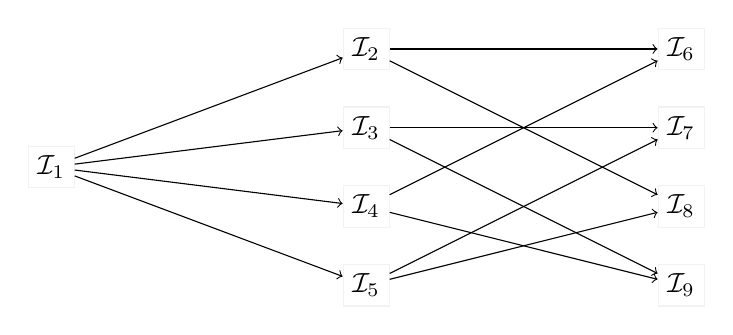
\begin{tikzpicture}
\draw (0,-3.5) node [rectangle,draw=gray!10,minimum height=0.2cm, minimum width=0.2cm, text centered] (I-1) {$\CalI_1$};

\foreach \id in {2,...,5}
	\draw (4,-\id) node  [rectangle,draw=gray!10,minimum height=0.2cm, minimum width=0.2cm, text centered] (I-\id) {$\CalI_\id$};
	
\foreach \id in {6,...,9}
	\draw (8,-\id+4) node  [rectangle,draw=gray!10,minimum height=0.2cm, minimum width=0.2cm, text centered] (I-\id) {$\CalI_\id$};
	
\foreach \id in {2,...,5} 
	\path[->] (I-1) edge (I-\id);

\path[->] (I-2) edge (I-6);
\path[->] (I-2) edge (I-8);
\path[->] (I-3) edge (I-7);
\path[->] (I-3) edge (I-9);
\path[->] (I-4) edge (I-6);
\path[->] (I-4) edge (I-9);
\path[->] (I-5) edge (I-7);
\path[->] (I-5) edge (I-8);

\end{tikzpicture}
\end{center}

Let us compute $\Phi_\CalP$ with $\CalI_1 = \langle \emptyset, \emptyset \rangle$:
\[
\begin{array}{lclcl}
\Phi_\CalP(\CalI_1) & = & \langle \{b\}, \emptyset \rangle & = & \CalI_4, \\
\Phi_\CalP(\CalI_4) & = & \langle \{a, b\}, \emptyset \rangle & = & \CalI_6, \\
\Phi_\CalP(\CalI_6) & = & \langle \{a, b\}, \emptyset \rangle & = & \CalI_6.
\end{array}
\]
The interpretation $\CalI_6$ is least fixed point of $\Phi_\CalP$, e.g. $\Lfp \Phi_\CalP = \CalI_6$, which also corresponds to the least model of $\WComp\CalP$.
\end{example}
\end{tcolorbox}
\vspace*{\fill}
\newpage

For a given set of candidate explanations $\CalC$, the set of positive candidate explanations, denoted by $\CalC^{pos}$, among the set of candidates is defined as  
\[
\begin{aligned}
\CalC^{pos} = \{\CalC_j \ | \ \CalC_j \in \CalC \mbox{ and } \CalP \cup \CalC_j \ModelsWCS \CalO\}.
\end{aligned}
\]
The set of negative candidate explanations, denoted by $\CalC^{neg}$, is given by $\CalC\setminus\CalC^{pos}$.
\end{definition}
\bigskip
\begin{prop} 
\label{prop:p0}
\normalfont
Let $\langle \CalP, \CalA_\CalP, \ModelsWCS \rangle$ be an \textit{abductive framework}, $\CalO$ an observation, and $\CalE \subseteq \CalA_\CalP$ an explanation for $\CalO$ which contains a complementary pair $c \leftarrow \top, c \leftarrow \bot$. Then, $\CalE'= \CalE \setminus \{c \leftarrow \bot\}$ is also an explanation for $\CalO$ and $\CalM_{\CalP \cup \CalE} = \CalM_{\CalP \cup \CalE'}$.
\begin{proof}
 \cite{corepaper}.
\end{proof}
\end{prop}
\bigskip
\begin{prop}
\label{prop:monotonicity}
\normalfont
Explanations are \textit{monotonic}. Let $\langle \CalP, \CalA_\CalP, \ModelsWCS \rangle$ be an abductive framework and $\CalO$ an observation. If $\CalE$ is an explanation for $\CalO$, then any set $\CalE'$ such that $\CalE \subseteq \CalE' \subseteq \CalA$ is also an explanation for $\CalO$.
\begin{proof}
\cite{holldobler2009logic}.
\end{proof}
\end{prop}

There are two possible ways of abductive reasoning: credulous and sceptical. In credulous reasoning all the consequences which follow from the program and at least one of the explanations for the observation are valid conclusions. On the other hand, in sceptical reasoning, a conclusion is only valid if it follows from the program and all the explanations for the observation. 

Let $\langle \CalP, \CalA_\CalP, \CalIC, \ModelsWCS\rangle$ be an abductive framework, $\CalO$ an observation and $\CalF$ a formula:
\begin{itemize}
\item $\CalF$ follows credulously from $\CalP$ and $\CalO$  if and only if there exists an explanation~$\CalE$ for $\CalO$ such that $\CalP \cup \CalE \ModelsWCS \CalF$.
\item $\CalF$ follows sceptically from $\CalP$ and $\CalO$ if and only if for all explanations~$\CalE$ for $\CalO$ we find $\CalP \cup \CalE \ModelsWCS \CalF$.
\end{itemize}

The set of sceptical consequences $\CalS_{\CalE}$ of a given set of explanations $\CalE$ is defined as follows
\[
\begin{array}{lcl}
\CalS_{\CalE} & = &  \underset{\CalE' \in \CalE}{\cap} \CalM_{\CalP \cup \CalE' } \\
		      & = &  \langle  \underset{\CalE' \in \CalE}{\cap} \CalM_{\CalP \cup \CalE' }^\top, \underset{\CalE' \in \CalE}{\cap} \CalM_{\CalP \cup \CalE'} ^ \bot \rangle.
\end{array}
\]

All the notions about the abductive framework, including the definition of candidate explanations and how to reason with respect to the weak completion of programs is presented in more details by Example~\ref{example:abduction} on page~\pageref{example:abduction}.

\subsection{Complexity}

\begin{prop}
\label{prop:hasexp}
\normalfont
Computing $\Lfp \Phi_\CalP$ can be done in polynomial time for acyclic logic programs $\CalP$.
\begin{proof}
See \cite{saldanha1872contextual}, Proposition 12.
\end{proof}
\end{prop}

\begin{prop}
\label{prop:hasexp}
\normalfont
Deciding whether an observation $\CalO$ has an abductive explanation based on a given program $\CalP$ and its respective set of abducibles~$\CalA_\CalP$ is NP-complete.
\begin{proof}
See \cite{saldanha1872contextual}, Proposition 13.
\end{proof}
\end{prop}

\begin{prop}
\label{prop:np}
\normalfont
Deciding whether $\CalP \cup \CalE \ModelsWCS \CalF$ does not hold for all explanations $\CalE$ given $\CalA_\CalP$ is NP-complete.
\begin{proof}
See \cite{saldanha1872contextual}, Proposition 14.
\end{proof}
\end{prop}

\begin{prop}
\label{prop:complement}
\normalfont
Let $\CalL \subseteq \sum^*$ be a language. Then $\CalL$ is NP-complete if and only if $\CalL$ is coNP-complete.
\begin{proof}
See \cite{papadimitriou2003computational}, Proposition 10.1.
\end{proof}
\end{prop}

\begin{prop}
\label{prop:hasexp}
\normalfont
Deciding whether $\CalP \cup \CalE \ModelsWCS \CalF$ holds for all explanations $\CalE$ given~$\CalA_\CalP$ is coNP-complete.
\begin{proof}
The opposite problem is shown to be NP-complete by Proposition~\ref{prop:np}. By Proposition~\ref{prop:complement}, deciding the above problem is coNP-complete.
\end{proof}
\end{prop}

\begin{definition}
\label{def:dp}
\normalfont
 A Language $\CalL$ is in the complexity class DP if and only if there are two languages $\CalL_1 \in \mbox{ NP}$ and $\CalL_2 \in \mbox{ coNP}$ such that $\CalL = \CalL_1 \cap \CalL_2$.
\end{definition}

\begin{prop}
\label{prop:hasexp}
\normalfont
The question whether $\CalF$ follows sceptically from an abductive problem is DP-complete.
\begin{proof}
See \cite{saldanha1872contextual}, Proposition 17.
\end{proof}
\end{prop}

\newpage
\vspace*{\fill}
\begin{tcolorbox}
\begin{example}
\label{example:abduction}
\normalfont
Consider program $\CalP$ consisting of the following clauses:
\[
\begin{array}{lcl}
c \leftarrow a. \\
c \leftarrow b.
\end{array}
\]
Assume that $\CalIC = \emptyset$ and that $\CalO = \{c\}$. Let us consider this observation in the abductive framework $\langle \CalP, \CalA_\CalP, \CalIC, \ModelsWCS\rangle$, where the set of abducibles $\CalA_\CalP$ consists of the following facts and assumptions:
\[
\begin{array}{ccccccc}
a &\leftarrow& \top. &\quad& a &\leftarrow& \bot.\\
b &\leftarrow& \bot. &\quad& b &\leftarrow& \bot.
\end{array}
\]
There are the following five non-complementary explanations for $\CalO$:
\[
\begin{array}{lcl}
\CalE_1 &=& \{a\leftarrow \top\}, \\
\CalE_2 &=& \{b \leftarrow \top\}, \\
\CalE_3 &=& \{a \leftarrow \top, b \leftarrow \bot\}, \\
\CalE_4 &=& \{a \leftarrow \bot, b \leftarrow \top\}, \\
\CalE_5 &=& \{a \leftarrow \top, b \leftarrow \top\}.
\end{array}
\]
The only minimal explanations for $\CalO$ are $\CalE_1$ and $\CalE_2$. As $a$ and $b$ does not follow from all the explanations, it does not follow sceptically, but only credulous, from $\CalP$ and $\CalO$. \\
\newline
The set of candidate explanations $\CalC$ for $\CalP$ and $\CalO$ is the power set of $\CalA_\CalP$. The set of non-complementary candidate explanations $\CalC_{\CalA_\CalP}^{nc}$ consists of the following nine candidates:
\[
\begin{array}{lcl}
\CalC_1 = \emptyset, &\quad\quad& \\
\CalC_2 = \{a \leftarrow \top\}, &\quad\quad& \CalC_2 = \{a \leftarrow \bot\}, \\
\CalC_4 = \{b \leftarrow \top\}, &\quad\quad& \CalC_5 = \{b \leftarrow \bot\}, \\
\CalC_6 = \{a \leftarrow \top, b \leftarrow \top\}, &\quad\quad& \CalC_7 = \{a \leftarrow \top, b \leftarrow \bot\}, \\
\CalC_8 = \{a \leftarrow \bot, b \leftarrow \top\}, &\quad\quad&\CalC_9 = \{a \leftarrow \bot, b \leftarrow \bot\}. \\
\end{array}
\]
The set of minimal candidate explanations for $\CalA_\CalP$ and $\CalO$, $\CalC_{\CalA_\CalP,\CalO}^{min}$, consists of the candidates $\CalC_1$, $\CalC_2$, $\CalC_3$, $\CalC_4$, $\CalC_5$ and $\CalC_9$. The set of positive candidate explanations $\CalC_{\CalA_\CalP,\CalO}^{min, pos}$ consists only of $\CalC_2$ and $\CalC_4$. Finally, the sceptical consequences of $\CalC_{\CalA_\CalP,\CalO}^{min, pos}$ is given by
\[
\CalS_{\CalC_{\CalA_\CalP,\CalO}^{min, pos}} = \langle \{a, c\} \cap \{b, c\}, \emptyset \cap \emptyset \rangle = \langle \{c\}, \emptyset \rangle
\]
\end{example}
\end{tcolorbox}
\vspace*{\fill}
\newpage

% -------------------------------------------------------------------------------------------------------------------------------------------------------------------------------------------------------------------------------------------------------------------------------------------- %
\section{Connectionist Networks}
\label{sec:preliminaries:cn}

A connectionist network consists of interconnected processing units. The general model of a processing unit consists of a summing part followed by an output part. The summing part receives N input values, weights each value, and computes a weighted sum. The weighted sum is called the \textit{activation value}. The sign of the weight for each input determines whether the input is \textit{excitatory} (positive weight) or \textit{inhibitory} (negative weight). The output part produces a signal from the activation value. 

We can divide these connectionist networks into two large classes. One class consists of the feed-forward networks and the other class consists of the recurrent networks. In general, whether a network belongs to one class or another can be decided based on its overall connectivity. If the network has one or more cycles, i.e., it is possible to follow a path from a unit to itself, then the network is referred to as recurrent. Feed-Forward networks have no cycles. 

We assume the reader to be familiar with connectionist networks as, for example, it is defined in \cite{feldman1982connectionist}. In particular, we will use McCulloch-Pitts networks of threshold units as defined in \cite{mcculloch1943logical} and multi-layer feed-forward networks as defined in \cite{rumelhart1986general}. We use modified connections of the following form:

\begin{itemize}

\item In case of a \textit{positively modified connection}, the input $i = wv$ of a unit is only received if the modifier $m$ is $1$, where $v$ is the output of the sending unit and $w$ is the weight of the connection:
\[
i = \left\{ 
\begin{array}{ll}
wv & \mbox{if } m=1, \\
0   & \mbox{if } m=0.
\end{array}
\right .
\]

\item In case of a \textit{negatively modified connection}, the input $i = wv$  is only received if the modifier $m$ is $0$:
\[
i = \left\{
\begin{array}{ll}
0 & \mbox{if } m=1, \\
wv & \mbox{if } m=0.
\end{array}
\right .
\]
\end{itemize}

The modifier $m$ is the output of another unit. Figure~\ref{fig:modifier} shows the graphical representations of a positively and a negatively modified connection. 

\begin{figure}
	\centering
	\begin{subfigure}{0.45\textwidth}
		\scalebox{.8}{\modifiedconnectionspassive}
  		 \caption{Negative modification.}
	\end{subfigure}
	\hspace{1cm}
	\begin{subfigure}{0.45\textwidth}
		\scalebox{.8}{\modifiedconnectionsactive}
   		\caption{Positive modification.}
	\end{subfigure}
	\caption{The output $v$ of unit $u_1$ is received by the input $i$ of unit $u_2$ only if the modifier $m$ of unit $u_3$ is 0 (a) or 1 (b), respectively.}
	\label{fig:modifier}
\end{figure}

\subsection{Recurrent Networks}
\label{sec:preliminaries:rcn}

The following notions introduced here are based on \cite{hertz1991introduction, medsker1999recurrent}. If the input in a feed-forward network is held constant, the trajectory of the network in state space will remain at a single point. Clearly, in order to archive interesting sequential behaviour in the presence of a constant input, there must be recurrent connections in the network. Therefore, because our main goal is to generate a sequence of candidate explanations for the abductive framework which characterises a sequential behaviour, we will focus on recurrent networks.

Recurrent networks were created in the 1980's and have been an important focus of research and development during the 1990's. They are designed to learn sequential or time-varying patterns, because each unit can use its internal memory to maintain information about the previous input. In cases of language, for example, if we would like to predict the next word in a sentence it is very important to know which words came before it. Thus, allowing the network to gain a deeper understanding of the statement is a great property when it comes to problems like this one. Language modelling is only one of the many applications for these recurrent networks. They have also been applied to image processing, pattern recognition, classification, clustering, data mining and so on.

The topology of a recurrent network can be very general, since they allow feedback connections. This means that every unit can be connected to every unit, including to itself. Allowing the presence of feedback connections among units brings an important characteristic to this networks, a time-dependent behaviour. Because of this, they can also be classified as dynamic networks. The state of a network, at one moment in time, also depends on the state at a previous moment in time. The dynamics of a recurrent neural network can be continuous or discrete in time. When a continuous time system is simulated, it is usually converted into a set of simple first order difference equations, which is formally identical to a discrete system. Therefore, we will concentrate on discrete time networks.

The dynamics of a recurrent network can be described, for instance, by a discrete time system 
\[
x(k + 1) = f(x(k)), \quad k \geq 1, 2,...,
\]
where $x$ denotes the state of the corresponding network and $f$ is some suitable mapping. 

The architecture of the recurrent network can vary from fully interconnected (Figure~\ref{fig:fullyconnected}) to partially connected (Figure~\ref{fig:partiallyconnected}). Fully connected networks do not have distinct input layers of nodes, and each unit has a weighted connection to every other unit in the architecture as well as a single feed-back connection to itself.

Simple partially recurrent networks (Figure~\ref{fig:partiallyconnected}) have distinct input layer of nodes and not every unit must be connected to every other unit. However, although some nodes are part of a feed-forward structure, other units provide the sequential context and receive feed-back connections from other units. These units are denoted the context units and composed what we will later refer to as the context layer. Weights from the context units (e.g., C1 and C2 in out example) are processed like those for the input units, for example, using back propagation. The context units receive time-delayed feedback from, in the case of Figure~\ref{fig:partiallyconnected}, the second layer units. Training data consists of inputs and their desired successor outputs. These type of networks can be trained, for example, to predict the next letter in a string of characters or to validate a string of characters.

\begin{figure}
	\centering
	\begin{subfigure}[b]{0.7\textwidth}
		\centering
		\scalebox{1.0}{\fullyconnected} 
		\bigskip
		\caption{\label{fig:fullyconnected} Fully connected.}
	\end{subfigure}
	\par\bigskip\par\bigskip\par\bigskip
	\begin{subfigure}[b]{0.7\textwidth}
		\centering
		\scalebox{1.0}{\partiallyconnected} 
		\bigskip
		\caption{\label{fig:partiallyconnected} Partially connected.}
	\end{subfigure}
	\par\bigskip
	\caption{Examples of a fully connected (a) and a partially connected (b) recurrent network. Solid lines represent trainable connections.}
\end{figure}

Back-propagation in feed-forward networks moves backward from the final error through the outputs, weights and inputs of each hidden layer, assigning those weights responsibility for a portion of the error by calculating their partial derivatives. These derivatives are then used by the learning rule, e.g. gradient descent, to adjust the weights up or down, depending on which direction decreases error.

Recurrent networks rely on an extension of back-propagation called back-propagation through time. Time, in this case, is simply expressed by a well-defined, ordered series of calculations linking one time step to the next, which is all back-propagation needs to work. Note that, Neural Networks, recurrent or not, are simply nested composite functions like $f(g(h(x)))$. Adding a time element only extends the series of functions for which we calculate derivatives with the chain rule.

In the sequel, the algorithm used will be the one developed in \cite{rumelhart1986leanrning}. The algorithm is a gradient search in weight space for a set of weights which implements the desired function. In \cite{rumelhart1986leanrning} the algorithm is demonstrated for nonrecurrent networks, but it can also be applied to recurrent networks.

To illustrate some of the ideas introduced here, a simple partially connected Recurrent Network consisting of two units is shown in Example~\ref{example:simplern} on page~\pageref{example:simplern}. Now we will now introduce two fundamental ways which can be used to add feed-back into feed-forward multi-layer networks, i.e. Jordan Networks and Elman networks. 

\subsection{Jordan Networks}
\label{sec:preliminaries:nn:jordan}

A theory of serial order which describes how sequences of actions might be learned and performed is presented in \cite{jordan1997serial}. The theory is embodied in the form of a parallel distributed processing \cite{rumelhart1986parallel} or connectionist network \cite{feldman1982connectionist}. Such networks are composed of many simple processing units that are connected though weighted links. The structure of the network consists of plan units, state units, hidden units and output units. The plan units and the state units together serve as the input units for a network which implements the output function $f$ through weighted connections from the plan and state units to the output units. The next-state function is implemented with recurrent connections from the output units to the state units. This allows the current state to depend on the previous state and on the previous output (which is itself a function of the previous state and the plan). The full overall structure of the network is shown in Figure~\ref{fig:jordan}.

In the proposed network, there is no explicit representation of temporal order and no explicit representation of action sequences. This is due to the fact that there is only one set of output units for the network, so that at any point in time, only one output vector is present. The network proposed by Jordan essentially implements the output function which relates patterns as a network associative memory in which many associations are stored in the same set of weights. The learning and generalisation of abilities demonstrated for such networks \cite{rumelhart1986parallel, rumelhart1981parallel} are just those that are needed for the output function.

Although it is possible that the next-state function is learned, this is not necessary for the system as a whole to be able to learn to produce sequences. Therefore, the recurrent connections have a fixed weight of 1.0 and all the other connections are trained. Learning is realised as an error-correcting process in which parameters of the network are incrementally adjusted based on the difference between the actual output of the network and the desired output. Essentially, the next-state function provides a time-varying state vector, and associations are learned from this state vector and plan vector to desired output vectors. 

The form that desired output vectors are assumed to take is a generalisation of the approach used in traditional error-correlation schemes. Instead of assuming that a value is specified for each output unit, it is assumed that there are constraints specified on the values of the output units. Constraints may specify a range of values that an output unit may have, a particular value, or no value at all. It is also possible to consider constraints that are defined among output units. For example, the sum of the activations of a set of units might be required to take on a particular value. More details on how these constraints enter into the learning process is given in \cite{jordan1997serial}.

\begin{figure}
\centering
\scalebox{1.0}{\jordangeneral}
\caption{\label{fig:jordan}A simple recurrent network in which activations are copied from the output layer to the context layer on a one-for-one basis, with fixed weight of 1.0. Solid lines represent trainable connections.}
\end{figure}

\subsection{Elman Networks}
\label{sec:preliminaries:nn:elman}

As introduced in \cite{elman1989representation} and \cite{elman1990finding}, an Elman Network is a three-layered recurrent network, with an additional set of units called the context layer. Both the input units and the context units activate the hidden units. The hidden units then feed forward to activate the output units and also feed back to activate the context units. This constitutes the forward activation. The output is then compared with the expected output for the given input and back propagation is used to adjust connection strengths incrementally. Recurrent connections are fixed at 1.0 and are not subject to adjustments.  The full overall structure of the network is shown in Figure~\ref{fig:elman}.

As one may notice, this approach is an variation of the Jordan Networks introduced in the previous Section. The only difference between them is on the source of the recurrent connections, which is the output layer and the hidden layer for Jordan and Elman networks, respectively. This is also the main characteristic of the Elman networks, which is an internal representation of time.

\newpage
\vspace*{\fill}
\begin{tcolorbox}
\begin{example}
\label{example:simplern}
\normalfont
An example of a simple partially connected recurrent network consisting of two units is shown below. 
\begin{center}
\scalebox{1.0}{\simplernn}
\end{center}
The recurrent connection of the output unit back to itself means that the output of the network depends not only on the input, but also on the state of the network at the previous time step.
\bigskip

For example, letting $\mu$ be the value of the recurrent weight, and assuming for simplicity that the units are linear ,i.e., the function is the identity function, the activation of the output unit at time t is given by
\[
x_2(t) = \mu x_2(t-1) + w_{21}x_1(t)
\]
where $x_1(t)$ is assumed to be constant over time. \\
\end{example}
\end{tcolorbox}
\vspace*{\fill}
\newpage

In feed-forward networks employing hidden units and a learning algorithm, the hidden units develop internal representations for the input patterns that recode those patterns in a way which enables the network to produce the correct output for a given input. In the architecture presented in \cite{elman1989representation}, the context units remember the previous internal state. Therefore, the hidden units have the task of mapping both an external input and the previous internal state to the desired output. Because the patterns on the hidden units are saved as context, the hidden units must accomplish this mapping and at the same time develop representations which are useful encodings of the temporal properties of the sequential input. Thus, the internal representations are now sensitive to temporal context.

\begin{figure}
\centering
\scalebox{1.0}{\elmangeneral}
\caption{\label{fig:elman}A simple recurrent network in which activations are copied from the hidden layer to the context layer on a one-for-one basis, with fixed weight of 1.0. Solid lines represent trainable connections.}
\end{figure} % INCLUDE: preliminaries
% !TEX root = ../thesis.tex

\chapter{Generating a Static Sequence of Candidate Explanations}
\label{sec:cn}

In the introduction we have briefly discussed a method using connectionist networks to compute the sceptical consequences of a given program $\CalP$ and its respective set of abducibles $\CalA_\CalP$ by means of abduction, which was introduced in \cite{corepaper}. This chapter will focus on the component of this network responsible for generating the candidate explanations for $\CalA_\CalP$. In particular, this component is a McCulloch-Pitts network \cite{mcculloch1943logical} which sequentially generates all non-complementary candidate explanations in a static pre-defined sequence. After explaining how this has been done, we would like to improve this approach by extending the current version of this network such that it will now generate only minimal candidate explanations.

\section{Non-Complementary Candidate Explanations}
\label{sec:cn:ncce}

Consider a program $\CalP$, its respective set of abducibles $\CalA_\CalP$, an observation $\CalO$ and an explanation $\CalE \subseteq \CalA_\CalP$ for $\CalO$ which contains a complementary pair of clauses, e.g. $c \leftarrow \top$ and $c \leftarrow \bot$. As it is stated in Proposition~\ref{prop:p0}, $\CalE'= \CalE \setminus \{c \leftarrow \bot\}$ is also an explanation for $\CalO$ and $\CalM_{\CalP \cup \CalE} = \CalM_{\CalP \cup \CalE'}$. From Proposition~\ref{prop:p0} we can then directly conclude that complementary explanations do not need to be considered. Because of this, we will start by focusing only on the generation of non-complementary candidate explanations.

For a given a program $\CalP$ containing $n$ undefined atoms, the set of abducibles $\CalA_{\CalP}$ consists of $2n$ facts and assumptions. There are $3^{2n}$ candidate explanations and $3^n$ non-complementary candidate explanations for $\CalA_{\CalP}$. As mentioned before, we will focus on the non-complementary candidates only which is already a significant optimisation on the number of candidates. This is illustrated in Example~\ref{example:suppression} on page~\pageref{example:suppression}. These candidate explanations can be represented by means of n-bit binary vectors, where $n = |\CalA_{\CalP}|$ and each bit represents one of the $n$ atoms or literals in $\CalA_{\CalP}$. For example, each candidate explanation in $\CalC_{\CalA_{\CalP_{sup}}}$ can be represented by a 4-bit binary vector.

\newpage
\vspace*{\fill}
\begin{tcolorbox}
\begin{example}
\label{example:suppression}
\normalfont 
Consider Byrne's suppression task discussed in the introduction. If we focus on the conditionals given Group II (Simple + Alternative), they can be represented by the program $\CalP_{sup}$ consisting of the following four clauses:
\[
\begin{array}{lcl}
l & \leftarrow & e \wedge \neg ab_1. \\
l & \leftarrow & t \wedge \neg ab_2. \\
ab_1 & \leftarrow & \bot. \\
ab_2 & \leftarrow & \bot.
\end{array}
\]
Where the atoms $l$, $e$, and, $t$ stand for \textit{she sill study late in the library}, \textit{she has an essay to finish}, and \textit{she has a text book to read}, respectively. Moreover, the atoms $ab_1$ and $ab_2$ stand for the abnormalities.

We can observe that only the atoms $e$ and $t$ are undefined. Thus, the set of abducibles~$\CalA_{\CalP_{sup}}$ consists of the following four facts and assumptions:
\[
\begin{array}{ccc}
e \leftarrow \top. & \quad & e \leftarrow \bot. \\
t \leftarrow \top. & \quad & t \leftarrow \bot.
\end{array}
\]
There are eighty-one candidates explanations for $\CalA_{\CalP_{sup}}$, where nine of them are non-complementary. The set of non-complementary candidate explanations $\CalC_{\CalA_{\CalP_{sup}}}$ consists of the following nine candidates:
\[
\begin{array}{lcl}
\CalC_0 = \emptyset, &\quad\quad& \\
\CalC_1 = \{e \leftarrow \top\}, &\quad\quad& \CalC_2 = \{e \leftarrow \bot\}, \\
\CalC_3 = \{t \leftarrow \top\}, &\quad\quad& \CalC_4 = \{t \leftarrow \bot\}, \\
\CalC_5 = \{e \leftarrow \top, t \leftarrow \top\}, &\quad\quad& \CalC_6 = \{e \leftarrow \top, t \leftarrow \bot\}, \\
\CalC_7 = \{e \leftarrow \bot, t \leftarrow \top\}, &\quad\quad&\CalC_8 = \{e \leftarrow \bot, t \leftarrow \bot\}. \\
\end{array}
\]
\end{example}
\end{tcolorbox}
\vspace*{\fill}
\newpage

The candidate explanation
\[
\CalC_0 = \emptyset
\]
is represented by 0000, and the candidate explanation
\[
\CalC_1 = \{e \leftarrow \top\}
\]
is represented by 1000. Table~\ref{table:4bitsvector} shows the 4-bit representation for each of the nine non-complementary candidate explanations in $\CalC_{\CalA_{\CalP_1}}$. Given this, the goal is to construct a neural network which sequentially generates the binary vectors shown in Table~\ref{table:4bitsvector}.

\begin{table}
\centering
\begin{tabular}{l|llll}
Candidate Explanations & $e^\top$ & $e^\bot$ & $t^\top$ & $t^\bot$\\
\hline
$\emptyset$ & 0 & 0 & 0 & 0 \\
$\{e \leftarrow \top \}$ & 1 & 0 & 0 & 0 \\
$\{e \leftarrow \bot \}$ & 0 & 1 & 0 & 0 \\
$\{t \leftarrow \top \}$ & 0 & 0 & 1 & 0 \\
$\{t \leftarrow \bot \}$ & 0 & 0 & 0 & 1 \\
$\{e \leftarrow \top,  t \leftarrow \top\}$ & 1 & 0 & 1 & 0 \\
$\{e \leftarrow \top,  t \leftarrow \bot\}$ & 1 & 0 & 0 & 1 \\
$\{e \leftarrow \bot,  t \leftarrow \top\}$ & 0 & 1 & 1 & 0 \\
$\{e \leftarrow \bot,  t \leftarrow \bot\}$ & 0 & 1 & 0 & 1\\
\end{tabular}
\bigskip
\caption{Binary vector definitions of the non-complementary candidate explanations for the set of abducibles $\CalA_{\CalP_1}$.}
\label{table:4bitsvector}
\end{table}

We start by formally specifying a finite automaton with state output (Moore machine)~\cite{moore1956gedanken} as shown in Figure~\ref{fig:41} on page~\pageref{fig:41}. This automaton has the set $\{0,1\}$ of input symbols, the set $\{0000,0001,0010,0100,1000,0101,1001,0110,1010\}$ of output symbols, the set $\{q_0,q_1,q_2,q_3,q_4,q_5,q_6,q_7,q_8\}$ of states with $q_0$ being the initial state, the following transition function $\delta$ and the output function $\lambda$:
\[
\begin{array}{c|cccc|c}
\delta & 0 & 1 &\quad\quad\quad\quad& state & \lambda\\ 
\cline{0-2}  \cline{5-6}
q_0 & q_0 & q_1 &\quad\quad\quad\quad& q_0 &0000\\
q_1 & q_1 & q_2 &\quad\quad\quad\quad& q_1 &1000\\
q_2 & q_2 & q_3 &\quad\quad\quad\quad& q_2 &0100\\
q_3 & q_3 & q_4 &\quad\quad\quad\quad& q_3 &0010 \\
q_4 & q_4 & q_5 &\quad\quad\quad\quad& q_4 &0001 \\
q_5 & q_5 & q_6 &\quad\quad\quad\quad& q_5 &1010\\
q_6 & q_6 & q_7 &\quad\quad\quad\quad&q_6 & 1001 \\
q_7 & q_7 & q_8 &\quad\quad\quad\quad& q_7 &0110\\
q_8 & q_8 & q_0 &\quad\quad\quad\quad&q_8 & 0101
\end{array} 
\]

\begin{figure}[t]
\begin{center}
\scalebox{.75}{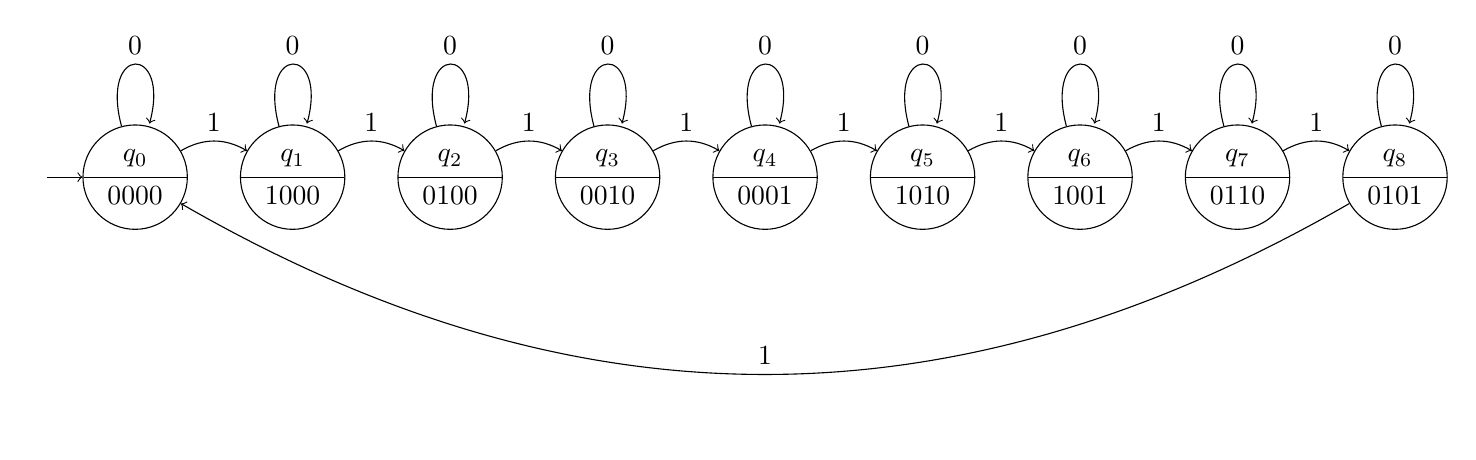
\begin{tikzpicture}[node distance = 20mm,initial text=,baseline=0mm]
  \node[state with output,draw,initial](q0){$q_0$ \nodepart{lower} $0000$};
  \node[state with output,draw](q1)[right of=q0]{$q_1$ \nodepart{lower} $1000$};
  \node[state with output,draw](q2)[right of=q1]{$q_2$ \nodepart{lower} $0100$};
  \node[state with output,draw](q3)[right of=q2]{$q_3$ \nodepart{lower} $0010$};
  \node[state with output,draw](q4)[right of=q3]{$q_4$ \nodepart{lower} $0001$};
  \node[state with output,draw](q5)[right of=q4]{$q_5$ \nodepart{lower} $1010$};
  \node[state with output,draw](q6)[right of=q5]{$q_6$ \nodepart{lower} $1001$};
  \node[state with output,draw](q7)[right of=q6]{$q_7$ \nodepart{lower} $0110$};
  \node[state with output,draw](q8)[right of=q7]{$q_8$ \nodepart{lower} $0101$};

  \path [->]  (q0) edge [loop above] node {$0$} ()
            (q0) edge [bend left]  node[above] {$1$} (q1)
            (q1) edge [loop above] node {$0$} ()
            (q1) edge [bend left] node[above] {$1$} (q2)
            (q2) edge [loop above] node {$0$} ()
            (q2) edge [bend left] node[above] {$1$} (q3)
            (q3) edge [loop above] node {$0$} ()
            (q3) edge [bend left] node[above] {$1$} (q4)
            (q4) edge [loop above] node {$0$} ()
            (q4) edge [bend left] node[above] {$1$} (q5)
            (q5) edge [loop above] node {$0$} ()
            (q5) edge [bend left] node[above] {$1$} (q6)
            (q6) edge [loop above] node {$0$} ()
            (q6) edge [bend left] node[above] {$1$} (q7)
            (q7) edge [loop above] node {$0$} ()
            (q7) edge [bend left] node[above] {$1$} (q8)
            (q8) edge [loop above] node {$0$} ()
            (q8) edge [bend left] node[above] {$1$} (q0);
\end{tikzpicture}}
\end{center}
\caption{\label{fig:41} A finite automaton generating all possible and non-complementary candidate explanations for $\CalA_{\CalP_2}$.}
\end{figure}

Warren McCulloch and Walter Pitts have shown in \cite{mcculloch1943logical} that each finite automaton with state output can be turned into a neural network of binary threshold units (sometimes called a \textit{McCulloch-Pitts network}) receiving an input via its input units and producing an output via its output units. In particular, a McCulloch-Pitts network to sequentially generate all the non-complementary candidate explanations for $\CalA_{\CalP_1}$ can be obtained from the finite automaton shown in Figure~\ref{fig:41}. 

The network has one input unit \textit{next} triggering the state transitions; nine internal units, which are called the hidden units; five output units, consisting of $e^\top$, $e^\bot$, $t^\top$, $t^\bot$ and \textit{done}, representing the four elements in the the set of abducibles $\CalA_{\CalP_1}$ and whether all the candidate explanations have been generated. The output unit \textit{done} is active when the last candidate is generated, and passive, otherwise. The network $\CalN_{\CalA_{\CalP_1}}$ is shown in Figure~\ref{fig:networkAP} and more details on how it has been constructed can be found in \cite{corepaper}. 

Note that, because our focus here is on the generation of candidate explanations, we only concentrate on one of the networks which compose the overall network described in \cite{corepaper}. The main goal of this network is to compute the sceptical abductive consequences for a given program $\CalP$ and observation $\CalO$.

Among the other components of this overall network, there is a network denoted by $e\CalN_{\CalP}$ which encodes the given program $\CalP$ and computes the~$\Lfp \Phi_\CalP$. The network $e\CalN_{\CalP}$ has as input the output of the network $\CalN_{\CalA_{\CalP}}$, which is a given non-complementary candidate explanation $\CalC$ for the set of abducibles $\CalA_\CalP$. The network $e\CalN_{\CalP}$ uses this to compute the $\Lfp \Phi_{\CalP\cup\CalC}$ and its result is given as output of the network. 

Once this network is done with the computation of $\Lfp \Phi_{\CalP\cup\CalC}$ and outputs the expected results, the overall network then requests a new candidate explanation by activating unit \textit{next} of the network $\CalN_{\CalA_{\CalP}}$ and the process is repeated until unit \textit{done} (\textit{done}) is active and there is no more candidate explanations to be considered. In this moment, there is another component of the network which considers all the outputs given by the network network $e\CalN_{\CalP}$ together with a given observation $\CalO$ and computes the sceptical consequences of it.

Considering the behaviour of the overall network and because we know that the computation of $\Lfp \Phi_{\CalP\cup\CalC}$ is not done in a fixed number of time steps, it is clear that units \textit{next} and \textit{done} are crucial to assure communications among the several components as well as to make sure that the candidate explanations will be generated on demand.

\begin{figure}[tp]
\begin{center}
\scalebox{1.0}{\NetworkAP}
\end{center}
\caption{McCulloch-Pitts network $\CalN_{\CalA_{\CalP_1}}$ designed to sequentially generate all the non-complementary candidate explanations for $\CalA_{\CalP_1}$.}
\label{fig:networkAP}
\end{figure}

Initially, unit $q_0$ will be active and all other units passive. As soon as unit \textit{next} is externally activated, then unit $q_0$ will become passive and unit $q_1$ will become active. Moreover, unit $q_1$ will activate unit $e^\top$ representing the first non-complementary and non-empty candidate explanation
\[
\CalC_1 = \{ e \leftarrow \top\}.
\] 
Upon further external activation of unit \textit{next}, this process will continue until unit $q_8$ becomes active. Unit $q_8$ will activate units $e^\bot$ and $t^\bot$ representing the last candidate explanation to be considered 
\[
\CalC_8 = \{e \leftarrow \bot,\ t \leftarrow \bot\}.
\]
Another activation of unit \textit{next} will return the network into its initial state. Because the environment needs to know when all possible explanations have been generated, the output unit \textit{done} will also become active once unit $q_8$ becomes passive. Unit \textit{done} will remain active unless unit \textit{next} is externally activated again. 

While the approach described here restricted the candidate explanations for a given set of abducibles to the non-complementary ones, it is well known that abduction often restricts this explanations to the minimal ones. Given this, we would like to introduce an extension of the current approach such that only the non-complementary and minimal candidate explanations are generated.

\section{Minimal Candidate Explanations}
\label{sec:cn:mce}

As mentioned before, it is often the case that one is interested in reasoning w.r.t. the minimal explanations. Intuitively, minimal explanations are interesting in the sense that they are not too general and do not trivially imply the given observation. In other words, the minimality property prevents from over-restricting the models of the abductive explanations.

From Proposition~\ref{prop:monotonicity} it directly follows that, for a given program $\CalP$, its respective set of abducibles $\CalA_\CalP$ and an observation $\CalO$, if $\CalE \subseteq \CalA_\CalP$ is an explanation for $\CalO$, i.e. $\CalP \cup \CalE \ModelsWCS \CalO$, then the explanation $\CalE$ with additional facts and assumptions is still an explanation for $\CalO$. This means that, when generating the non-complementary candidate explanations, we can avoid the generation of candidates which are a superset of those candidates known to have explained the given observation. In this way, no candidate $\CalC$ such that $\CalE \subseteq \CalC$ and $\CalP \cup \CalE \ModelsWCS \CalO$ should be generated.

Thus, the goal now is to construct a network which will restrict the generation of non-complementary candidate explanations to the minimal ones. One way to archive this is by extending the network $\CalN_{\CalA_{\CalP_1}}$ shown in Figure~\ref{fig:networkAP}. For this purpose, reconsider the program $\CalP_{sub}$ from Example~\ref{example:suppression} on page~\pageref{example:suppression}. Because the minimal explanations are defined w.r.t. a given observation, let's consider a specific observation, e.g. \textit{she goes to the library},
\[
\CalO_1 = \{l\}.
\]
There are only two minimal explanations for $\CalO_1$ given $\CalP_1$, i.e. 
\[
\begin{array}{lcl}
\CalE_1 & = & \{e \leftarrow \top\}, \\
\CalE_2 & = & \{t \leftarrow \top\}. 
\end{array}
\]

In this case, instead of sequentially generating all the nine binary vectors representing each of the non-complementary candidate explanations as it is done by the network $\CalN_{\CalA_{\CalP_1}}$, we would like to have a network which would avoid the generation of those binary vectors representing the candidate explanations which are supersets of candidates known to be explanations. The candidate explanations $\CalC_1$ and $\CalC_3$ are equal to the minimal explanations $\CalE_1$ and $\CalE_2$, respectively. Because of this, we know that they are explanations for the observation $\CalO_1$ and the extended network should not generate the candidate explanations
\[
\begin{array}{lclclcl}
\CalC_5 &=& \{e \leftarrow \top, t \leftarrow \top\},\\
\CalC_6 &=& \{e \leftarrow \top, t \leftarrow \bot\},\\
\CalC_7 &=& \{e \leftarrow \bot, t \leftarrow \top\}, 
\end{array}
\]
since $\CalC_1 \subseteq \CalC_5$, $\CalC_1 \subseteq \CalC_6$, $\CalC_3 \subseteq \CalC_5$, and $\CalE_3 \subseteq \CalC_7$. 

This means that after generating the candidate explanation 
\[\CalC_4 = \{t \leftarrow \bot\},
\]
the network is expected to avoid the generation of candidates which are a superset of already known explanations, which in this case are $\CalC_1$ and $\CalC_2$, and directly jump to the generation of the last candidate explanation
\[
\CalC_8 = \{e \leftarrow \bot, t \leftarrow \bot\}.
\]
Moreover, the network should then return to its initial state. Given this, the extended network is then expected to generate the following sequence of 4-bit binary vectors: 0000, 1000, 0100, 0010, 0001 and 0101.

Now, in order to obtain the network $\CalN'_{\CalA_{\CalP_1}}$ which will be an extension of $\CalN_{\CalA_{\CalP_1}}$ such that the generation of candidate explanations is no longer restricted only to non-complementary, but also to the minimal ones, we will apply the following three steps:

\begin{enumerate}
\item Access the information of whether the last candidate explanation generated has indeed explained the given observation and keep it during the upcoming time steps until all the candidate explanations have been generated;
\item For each candidate explanation, store the information of whether any other candidate explanation which is a subset of it has been in fact an explanation for the given observation;
\item Use the information from step 2 to avoid the generation of non-minimal candidate explanations.
\end{enumerate}

The first modification can be done by simply adding a new input unit $e$ (\textit{explanation}), which will be externally activated when the last possible explanation generated was in fact an explanation for the given observation. This means that unit $e$ will be active when that is the case, and passive, otherwise. Unit $e$ also has a recurrent connection which is negatively modified by unit \textit{next}. With this we make sure that, once unit $e$ has been activated, it will remain active also during the following time steps where unit \textit{next} is passive and, on the next time step where unit \textit{next} is active again, $e$ just remains active if it is externally activated.

Regarding the second step, the first candidate explanation to be generated
\[
\CalC_0 = \emptyset
\]
is a subset of all the other candidates. Because of this, we will add a connection from unit $q_0$ to unit \textit{done} which will be positively activated by units \textit{next} and $e$. This means that when the candidate $\CalC_0$ is an explanation for the given observation $\CalO$, no further candidate explanations will be generated and the network is done. Besides this, we also make the connection between $q_0$ and $q_1$ being positively modified by unit \textit{next} and negatively modified by unit $e$. Meaning that, for the case where~$\CalC_0$ is not an explanation for the given observation $\CalO$, the network will proceed as before and unit $q_1$ will be activated.

For the candidate explanations with cardinality equal or greater than two, the second step will be done by adding a corresponding unit $h_i$ for each of this candidates. Each of these units will be passive when its respective possible explanation should be generated and active, otherwise. This will be done by connecting each unit $q_j$ responsible for generating a subset of a given set to its respective unit $h_i$. By doing this, a given unit $h_i$ will be active as soon as any of its subsets is known to be an explanation. 

Another important point to be considered in the second step is that, once these units $h_i$ have been activated by one of units $q_i$, they need to remain active in the further time steps. This is important because the candidate explanations which are supersets of a given candidate explanation may not be generated directly after them, but in a few time steps later. Thus, this information should also be available in further time steps. 

Besides this, since we're creating new units representing only the candidate explanations which have cardinality greater than one, this candidates have at least two non-empty subsets, but only one of them being an actual explanation is sufficient to keep this candidate explanation from being generated. Thus, once one of the subsets of the given candidate is an explanation, unit should be active and remain active independent of the other subsets being indeed explanations or not. 

In practice, this can be done by simply adding a recurrent connection to each of these units. Each of this recurrent connections is negatively modified by unit \textit{done} such that they all become passive as soon as the last possible explanation has been generated.

In our example, four units $h_5$, $h_6$, $h_7$ and $h_8$ will be added for each of its respective candidate explanation
\[
\begin{array}{ccc}
\CalC_5 &=& \{e \leftarrow \top, t \leftarrow \top\},\\
\CalC_6 &=& \{e \leftarrow \top, t \leftarrow \bot\}, \\
\CalC_7 &=& \{e \leftarrow \bot, t \leftarrow \top\}, \\
\CalC_8 &=& \{e \leftarrow \bot, t \leftarrow \bot\}.
\end{array}
\]
Because units $q_1$ and $q_3$ are responsible for, respectively, generating the two candidate explanations 
\[
\begin{array}{ccc}
\CalC_1 = \{e \leftarrow \top\}, \\
\CalC_3 = \{t \leftarrow \top\}, \\
\end{array}
\]
there will be a connection from units $q_1$ and $q_3$ to unit $h_5$, since both $\CalC_1$ and $\CalC_3$ are subsets of $\CalC_5$ which is represented by unit $h_5$. For analogous reasons, there will be connections from units $q_1$ and $q_4$ to unit $h_6$, from units $q_2$ and $q_3$ to unit $h_7$, and from units $q_2$ and $q_4$ to unit $h_8$. Besides this, the four units $h_5$, $h_6$, $h_7$ and $h_8$ will have a self connection negatively modified by unit \textit{done}.
 
Finally, the third step regarding the fact that the network should be able to jump over the non-minimal possible explanations will be done in the following way. Each unit $q_i$ connected to a unit $q_{i+1}$ responsible for activating the generation of a possible explanation of cardinality greater than one will no longer be connected only to the next unit $q_{i+1}$, but to unit \textit{done} and to all units $q_j$ such that j = 0 or j > i. Besides this, we will make use of the $h_i$ units to positively or negatively modify each of these connections depending on the case. A connection from a unit $q_i$ to a unit $q_j$ will be positively modified by all units $h_k$ such that k < j, and negatively modified by unit $h_j$. Algorithm~\ref{alg:dependencies} shows the general steps for this modification, where PositiveConnection(a,b,c) and NegativeConnection(a,b,c) are used to express when a connection from unit a to unit b is positively and negatively modified by c, respectively.
In our case, for example, unit $q_4$ will no longer be connected only to unit $q_5$, but to units $q_5$, $q_6$ $q_7$, $q_8$, $q_0$ and \textit{done}. Unit $q_5$ will now be connected to units $q_6$, $q_7$ $q_8$, $q_0$ and \textit{done}. And so on, until unit $q_7$ which will be connected to units $q_8$, $q_0$ and \textit{done}. In our example, the algorithm would use \textit{min} equals to five and max equals to eight. To illustrate how the algorithm works, let's consider the connections from unit $q_4$ and see how they would be modified by units $h_i$. 

First of all, the connection from unit $q_4$ to unit $q_5$ will be negatively activated by unit $h_5$. This means that unit $h_5$ is passive when none of the following two candidate explanations are actual explanations for the observation~$\CalO$:
\[
\begin{array}{ccc}
\CalC_1 &=& \{e \leftarrow \top\},\\
\CalC_3 &=& \{t \leftarrow \top\}.
\end{array}
\]
In that case, unit $q_5$ is activated and the next candidate explanation to be generated is, as before, 
\[
\CalC_5 = \{e \leftarrow \top, t \leftarrow \top\}.
\]
The connection from unit $q_4$ to unit $q_6$ is positively modified by unit $h_5$ and negatively modified by unit $h_6$. This means that unit $h_5$ is active when one of the candidate explanations $\CalC_1$ or $\CalC_2$ (or both) were actual explanations for the observation $\CalO$.

\begin{tcolorbox}
\begin{algorithm}
\label{alg:dependencies}
\normalfont 
How to make the new connections between units $q_i$ and from them to unit \textit{done} be positively or negatively modified by units $h_i$.

\begin{algorithmic}[1]
\REQUIRE min = the smallest i from the $h_i$ units\\
\hspace{0.5cm} max = the greatest i from the $h_i$ units
\ENSURE Positive and negative modifications by units $h_i$ of the new connections between units $q_i$ and to unit \textit{done}
\bigskip
\WHILE {AddModifiers(min, max)}
	\FOR{$i \in \{min-1,\dots,max-1\}$} 
		\FOR {$j \in \{i+1,\dots,max\}$} 
			\FOR {$k \in \{i+1,\dots,j-1\}$} 
				\STATE PositiveConnection($q_i$, $q_j$,$h_k$)
			\ENDFOR
			\STATE NegativeConnection($q_i$, $q_j$,$h_j$)
		\ENDFOR
		\FOR {$j \in \{min,\dots,max\}$} 
			\STATE PositiveConnection($q_i$, $q_0$,$h_j$) and PositiveConnection($q_i$, $d$,$h_j$)
		\ENDFOR
	\ENDFOR
\ENDWHILE
\end{algorithmic}
\end{algorithm}
\end{tcolorbox}

Consequently, the next candidate explanation should no longer be $\CalC_5$. If that is case, since the connection from unit $q_4$ to unit $q_5$ is negatively modified by unit $h_5$, unit $q_5$ will indeed not be activated. Besides this, unit $q_6$ is activated when none of the following two candidate explanations are actual explanations for the observation~$\CalO$:
\[
\begin{array}{ccc}
\CalC_1 &=& \{e \leftarrow \top\},\\
\CalC_4 &=& \{t \leftarrow \bot\}.
\end{array}
\]
If that is the case, the next candidate explanation to be generated is now
\[
\CalC_6 = \{e \leftarrow \top, t \leftarrow \bot\}.
\]
And so on, until the connections from unit $q_4$ to units $q_0$ and \textit{done}, which will be positively modified by units $h_5$, $h_6$, $h_7$ and $h_8$, meaning that when none of the remaining candidate explanations should be generated, i.e. all the four $h_i$ units are active, units \textit{done} and $q_0$ will be activated. Moreover, the activation of unit \textit{done} will deactivate units $h_i$ and the network is back to its initial state. The connections from unit $q_6$ to units $q_7$, $q_8$, $q_0$ and \textit{done}, from unit $q_7$ to units $q_8$, $q_0$ and \textit{done}, and from unit $q_8$ to units $q_0$ and \textit{done} will be positively or negatively modified by units $h_i$ following the same structure as explained above.

The connection from unit $q_4$ to unit $q_6$ is positively modified by unit $h_5$ and negatively modified by unit $h_6$. This means that unit $h_5$ is active when one of the candidate explanations $\CalC_1$ or $\CalC_2$ (or both) were actual explanations for the observation $\CalO$. Consequently, the next candidate explanation should no longer be $\CalC_5$. If that is case, since the connection from unit $q_4$ to unit $q_5$ is negatively modified by unit $h_5$, unit $q_5$ will indeed not be activated. Besides this, unit $q_6$ is activated when none of the following two candidate explanations are actual explanations for the observation~$\CalO$:
\[
\begin{array}{ccc}
\CalC_1 &=& \{e \leftarrow \top\},\\
\CalC_4 &=& \{t \leftarrow \bot\}.
\end{array}
\]
If that is the case, the next candidate explanation to be generated is now
\[
\CalC_6 = \{e \leftarrow \top, t \leftarrow \bot\}.
\]
And so on, until the connections from unit $q_4$ to units $q_0$ and \textit{done}, which will be positively modified by units $h_5$, $h_6$, $h_7$ and $h_8$, meaning that when none of the remaining candidate explanations should be generated, i.e. all the four $h_i$ units are active, units \textit{done} and $q_0$ will be activated. Moreover, the activation of unit \textit{done} will deactivate units $h_i$ and the network is back to its initial state. The connections from unit $q_6$ to units $q_7$, $q_8$, $q_0$ and \textit{done}, from unit $q_7$ to units $q_8$, $q_0$ and \textit{done}, and from unit $q_8$ to units $q_0$ and \textit{done} will be positively or negatively modified by units $h_i$ following the same structure as explained above.

A fragment of the network $\CalN_{\CalA_{\CalP_1}}$ is shown in Figure~\ref{fig:networkAPExtension} with all the necessary modifications to extend this network such that it will only generate the minimal candidate explanations. In order to get the final version of the extended network $\CalN'_{\CalA_{\CalP_1}}$, one needs to overlap the network $\CalN_{\CalA_{\CalP_1}}$ with the extensions shown in Figure~\ref{fig:networkAPExtension}.

So, after applying all the above described modifications to the network $\CalN_{\CalA_{\CalP_1}}$, we get the extended network $\CalN'_{\CalA_{\CalP_1}}$. The network $\CalN'_{\CalA_{\CalP_1}}$ has the same two input units \textit{done} and \textit{next} as before and an extra input unit $e$ (\textit{explanation}), which gives us the information whether the previous candidate was indeed an explanation. The hidden units now consist of units $q_i$ as before and the extra units $h_i$, which will be used to positively or negatively modify certain connections of the network. Units $h_i$ are the most important modification of the network and are the ones responsible for blocking non-minimal candidate explanations from being generated. The output units remain the same, i.e. five output units $e^\top$, $e^\bot$, $t^\top$, $t^\bot$ and \textit{done}. The connections between units $q_i$ and the output units $e^\top$, $e^\bot$, $t^\top$, $t^\bot$ also remain the same. The network $\CalN'_{\CalA_{\CalP_1}}$ generates all the minimal candidate explanations for the program $\CalP_1$ and a given observation $\CalO$.

\begin{figure}
\centering
\scalebox{0.5}{\NetworkAPExtension}
\caption{Fragment of the McCulloch-Pitts network from Figure~\ref{fig:networkAP} consisting of the necessary modifications to sequentially generate all the minimal candidate explanations for $\CalA_{\CalP_1}$.}
\label{fig:networkAPExtension}
\end{figure}

Let's observe how the network $\CalN_{\CalA_{\CalP_1}}'$ behaves for the observation
\[
\CalO_1 = \{l\}.
\]
As before, unit $q_0$ will be initially active and all other units passive. As soon as unit \textit{next} is externally activated, then unit $q_0$ will become passive and unit $q_1$ will become active. Moreover, unit $q_1$ will activate unit $e^\top$ representing the first minimal and non-empty candidate explanation 
\[
\CalC_1 = \{ e \leftarrow \top\}.
\]
Because $\CalC_1$ is an explanation for the observation $\CalO_1$, the next time unit \textit{next} is activated, unit $e$ will also be activated. Thus, units $q_2$, $h_5$ and $h_6$ will become active and unit $q_1$ will become passive. Moreover, unit $q_2$ will activate unit $e^\bot$ representing the candidate explanation
\[
\CalC_2 = \{ e \leftarrow \bot\}.
\]
In the next activation of unit \textit{next}, because $\CalC_2$ is not an explanation for the observation~$\CalO_1$, unit $e$ will be passive. Unit $q_2$ will become passive, unit $q_3$ will become active and units $h_5$ and $h_6$ will remain active. Moreover, unit $q_3$ will activate unit $t^\top$ representing the candidate explanation
\[
\CalC_3 = \{ t \leftarrow \top\}.
\]
In the next activation of unit \textit{next}, because $\CalC_3$ is also an explanation for the observation $\CalO_1$, unit $e$ will also be activated. Unit $q_3$ will become passive, units $q_4$ and $h_7$ will become active, and units $h_5$ and $h_6$ will remain active. Moreover, unit $q_4$ will activate unit $t^\bot$ representing the candidate explanation
\[
\CalC_4 = \{ t \leftarrow \bot\}.
\]
In the next time unit \textit{next} is activated, because $\CalE_4$ is not an explanation for the observation $\CalO_1$, unit $e$ will be passive. Unit $q_4$ will become passive and units $h_5$, $h_6$ and $h_7$ will remain active. Because units $h_5$, $h_6$ and $h_7$ are active, but unit $h_8$ is passive, unit $q_4$ will activate unit $q_8$. Unit $q_8$ will activate units $e^\bot$ and $t^\bot$ representing the candidate explanation
\[
\CalC_8 = \{e \leftarrow \bot, t \leftarrow \bot\}.
\]
Finally, the next time unit \textit{next} is activated, because $\CalC_8$ is not an explanation for the observation $\CalO_1$, unit $e$ will be passive. Moreover, unit $q_8$ will activate units $q_0$ and \textit{done}, and unit $q_8$ will become passive. Because unit \textit{done} is active, all units $h_i$ which were active, e.g. $h_5$, $h_6$ and $h_7$, will become passive, returning the network to its initial state and informing the environment that all possible explanations have been generated. This steps are shown in Table~\ref{table:networkstate}.

\begin{table}
\resizebox{\textwidth}{!}{\begin{minipage}{\textwidth}
\centering
\begin{tabular}{c|c|c}
Input & Hidden & Output\\ 
\hline
$t \ e$ & $q_0 \ q_1 \ q_2 \ q_3 \ q_4 \ q_5 \ q_6 \ q_7 \ q_8 \ h_5 \ h_6 \ h_7 \ h_8$ & $e^\top \ e^\bot \ t^\top \ t^\bot \ d$ \\
\hline
0 0 & 1 \ 0 \ 0 \ 0 \ 0 \ 0 \ 0 \ 0 \ 0 \ 0 \ 0 \ 0 \ 0 \ 0 & 0 \ \  0 \ \  0 \ \  0 \ \ 0 \\
1 0 & 0 \ 1 \ 0 \ 0 \ 0 \ 0 \ 0 \ 0 \ 0 \ 0 \ 0 \ 0 \ 0 \ 0 & 1 \ \  0 \ \  0 \ \  0 \ \ 0 \\
1 1 & 0 \ 0 \ 1 \ 0 \ 0 \ 0 \ 0 \ 0 \ 0 \ 0 \ 1 \ 1 \ 0 \ 0 & 0 \ \  1 \ \  0 \ \  0 \ \ 0 \\
1 0 & 0 \ 0 \ 0 \ 1 \ 0 \ 0 \ 0 \ 0 \ 0 \ 0 \ 1 \ 1 \ 0 \ 0 & 0 \ \  0 \ \  1 \ \  0 \ \ 0 \\
1 1 & 0 \ 0 \ 0 \ 0 \ 1 \ 0 \ 0 \ 0 \ 0 \ 0 \ 1 \ 1 \ 1 \ 0 & 0 \ \  0 \ \  0 \ \  1 \ \ 0 \\
1 0 & 0 \ 0 \ 0 \ 0 \ 0 \ 0 \ 0 \ 0 \ 0 \ 1 \ 1 \ 1 \ 1 \ 0 & 0 \ \  1 \ \  0 \ \  1 \ \ 1 \\
\end{tabular}
\bigskip
\caption{State of the input, hidden and output units of the network $\CalN'_{\CalA_{\CalP_1}}$ for the observation $\CalO_1 = \{l\}$ on its initial state and on the activation of the input unit \textit{next} for five consecutive time steps.}
\label{table:networkstate}
\end{minipage} }
\end{table}

With this we have shown in details one possible way of extending the network $\CalN_{\CalA_{\CalP_1}}$ to a network $\CalN'_{\CalA_{\CalP_1}}$ which will only compute the minimal candidate explanations for the given program $\CalP_1$ and any given observation $\CalO$. We have also explained how the network $\CalN'_{\CalA_{\CalP_1}}$ behaves for the observation
\[
\CalO_1 = \{l\}.
\]

Although we have focused in the previous example, one should remember that the network here presented is a general approach for any given program $\CalP$ which has a respective set of abducibles of size four. Figure~\ref{fig:exptree} shows the different outcomes the network $\CalN'_{\CalA_{\CalP}}$ can provide depending on the given program $\CalP$ and observation~$\CalO$. We use dashed arrows to denote that the previous candidate explanations did not explain the given observation and solid arrows to denote the opposite. For example, in the example where we consider the program $\CalP_1$ and the observation $\CalO_1$, the network output corresponds to the following path:
\[
0000 \DashedArrow[->,densely dotted] 1000 \rightarrow 0100 \DashedArrow[->,densely dotted] 0010 \rightarrow 0001 \DashedArrow[->,densely dotted]  0101 \DashedArrow[->,densely dotted] done.
\]

\begin{figure}
\scalebox{0.5}{ \candidatestree }
\bigskip
\caption{All the possible sequences of minimal candidate explanations for potential programs having a respective set of abducibles of size four taking into account potential arbitrary observations. Solid and dashed arrows denote positive and candidates, respectively. Wavy arrows denote the cases where both are possible.}
\label{fig:exptree}
\end{figure}

Example~\ref{example:additional} on page~\pageref{example:additional} shows another example of a program with a corresponding set of abducibles of size four and how the same network could be reused. Moreover, a network for a given program $\CalP$ which has a correspondent set of abducibles of arbitrary size can be constructed following the same structure. The details on how this can be done is explained earlier in this section where we present Algorithm~\ref{alg:dependencies} on page~\pageref{alg:dependencies}.

\newpage
\vspace*{\fill}
\begin{tcolorbox}
\begin{example}
\label{example:additional}
\normalfont 
Consider program $\CalP$ consisting of the following clauses:
\[
\begin{array}{lcl}
a &\leftarrow& b \\
a &\leftarrow& \neg b \\
a &\leftarrow& c \\
\end{array}
\]
The corresponding set of abducibles $\CalA_{\CalP_2}$ consists of the following four facts and assumptions:
\[
\begin{array}{ccc}
b \leftarrow \top &\quad& b \leftarrow \bot \\
c \leftarrow \top &\quad& c \leftarrow \bot \\
\end{array}
\]
It is easy to see that the network would look the same, with the only difference that units before representing $e^\top$, $e^\bot$, $t^\top$ and $t^\bot$ now represent $b^\top$, $b^\bot$, $c^\top$ and~$c^\bot$, respectively. If we now consider the observation
\[
\CalO_2 = \{a\},
\]
as the minimal explanations for $\CalO_2$ given $\CalP_2$ are the following
\[
\begin{array}{lcl}
\CalE_1 &=& \{b\}, \\
\CalE_2 &=& \{\neg b\}, \\
\CalE_3 &=& \{c\},
\end{array}
\]
one can see that, in this case, the output of the network would correspond to the following path from the tree shown in Figure~\ref{fig:exptree}:
\[
0000 \DashedArrow[->,densely dotted] 1000 \rightarrow 0100 \rightarrow 0010 \rightarrow 0001 \DashedArrow[->,densely dotted] done.
\]
\end{example}
\end{tcolorbox}
\vspace*{\fill}
\newpage

\section{Conclusion}

In this chapter we have focused on how to generate possible abductive explanations for a given program $\CalP$ and observation $\CalO$ using connectionist networks. First, we have looked into an approach to generate non-complementary explanations introduced in \cite{corepaper}. Then, we proposed a way to improve this approach by applying some modifications to it such that only minimal explanations are generated. Our new approach produces all possible explanations in a specific order such that minimal explanations can be detected and all non-minimal possible explanations can be discarded. This was a relevant improvement, since detecting minimality is not a trivial task, but it is still not the ideal solution to our problem for the following reasons.

First, although a formal specification of how to construct and extend this network is provided, the construction of different networks may be required for different sets of abducibles. This is certainly not the most convenient solution to our problem and therefore we would like to come up with a more general approach.

Besides this, we do not believe that humans test all possible explanations in a systematic way. It appears to us that in particular reasoning episodes some possible explanations are systematically tested whereas others are not considered at all. Our approach to generate the minimal candidate explanations already partially solves this problem in the sense that many unnecessary candidate explanations are discarded and, even for the same set of abducibles, the possible explanations vary depending on the given observation. However, the process of generating this possible explanations is still somehow done in a systematic way.

Given that, we would like to have a more general approach not only in the sense that it should be flexible and work for different sets of abducibles, but also by generating as possible explanations only those which are more plausible to actually explain our observations.

\label{sec:cn:conclusion}
	% INCLUDE: connectionist networks
% !TEX root = ../thesis.tex

\chapter{Learning Arbitrary Sequences of Candidate Explanations}
\label{sec:nn}

In Section~\ref{sec:cn} we have presented an approach for generating candidate explanations in a fixed given order. However, as we cannot assume that humans generate candidates in a static sequence, having an approach which is more abstract and can learn arbitrary sequences would be the ideal scenario. Therefore, in this chapter we will focus on recurrent networks, more specifically in Jordan and Elman networks. We will show how these networks can be used to archive the same results presented for the previous approach, but also how they can easily be generalised for arbitrary sequences.

\section{Non-Complementary Candidate Explanations}
\label{sec:nn:ncce}

In Section~\ref{sec:cn} we have shown by means of an example how a predefined sequence of non-complementary candidate explanations can be generated based on connectionist networks. Now we would like to start this section by showing that the same result can also be archived based on recurrent networks. In order to do so, we will begin by constructing, training and testing a recurrent network for the same example used before. Thus, reconsider the program $\CalP_{sup}$ presented in Example~\ref{example:suppression} on page ~\pageref{example:suppression}.

In the first version of the connectionist network presented before, each of the nine candidate explanations is generated one after the other in a fixed order. After generating the last one, unit \Done is activated and the network returns to its initial state. Every time a new candidate explanation is generated, the state of the network remains the same until a next candidate is requested by the activation of unit \textit{next}. This means that the expected output is the previous candidate explanation when unit \textit{next} is passive and the next one, otherwise.

One possible way to translate this problem into a temporal domain problem is by constructing a sequence of binary vectors consisting of five bits. The first four bits (from left to right) will correspond to the four output units of the connectionist network, representing $e^\top$, $e^\bot$, $t^\top$ and $t^\bot$. The last bit (from left to right) corresponds to unit \Done of the connectionist network, representing whether all the non-complementary candidate explanations have been generated. Each of these bits will be equal to \textit{one} when its respective unit is active and equal to \textit{zero} when it is passive.

Given this, there are different sequences we could obtain depending on the oscillation of the values of the request unit \textit{next}. As explained in Chapter~\ref{sec:cn}, we are just working with one component of a network which generated the sceptical consequences of a given program $\CalP$ and observation $\CalO$. Therefore, the activation of unit \textit{next} will come from the other components of this overall network which is responsible for checking weather a given candidate explanation $\CalC$ explains $\CalO$ given $\CalP$.

If we consider the scenario where the network only needs one time step to decide whether the candidate was an explanation, then next candidates would be requested one after another without a break. In that case we have the most basic sequence, which is the request sequence where unit \textit{next} is active for nine time steps in a row. For this sequence of values for the request unit, the output sequence expected is the following: 
\[
00000, 10000, 01000, 00100, 00010, 10100, 10010, 01100, 01011.
\]

However, this is not always the case since we don't know how many time steps the external network will need before requesting a next candidate explanation. Moreover, this steps are not fixed, meaning that for different candidates it might take a different number of time steps. Therefore, we can also obtain any sequence which has the following form: 
\[
\begin{array}{lllll}
(00000)^+,&(10000)^+, &(01000)^+, &(00100)^+, &(00010)^+,\\
	        &(10100)^+, &(10010)^+, &(01100)^+, &(01011)^+.
\end{array}
\]

The main task here is to predict, at each point in time, the next binary vector in the sequence which represents the next candidate explanation. The value of this vector will depend on two factors: the last candidate explanation generated and the value of unit \textit{next}. Thus, our input will also consist of a 5-bit binary vector where the first four bits (from left to right) also correspond to $e^\top$, $e^\bot$, $t^\top$ and $t^\bot$, but the last bit (from left to right) corresponds to unit \textit{next} of the connectionist network, representing the request of a new candidate explanation. This bit will be equal to \textit{one} when a new candidate explanation should be generated and \textit{zero}, otherwise. All possible inputs and its respective expected outputs can be seen in Table~\ref{table:trainingexplanations}.

\begin{table}
		\centering
	\begin{subtable}[h]{0.30\textwidth}
		\centering
		\begin{tabular}{cc}
		Input & Output \\
		\hline
		00000 & 00000 \\
		10000 & 10000 \\
		01000 & 01000 \\
		00100 & 00100 \\
		00010 & 00010 \\
		10100 & 10100 \\
		10010 & 10010 \\
		01100 & 01100 \\
		01010 & 01011 \\
		\end{tabular}
		\bigskip
		\caption{Cases where the fifth bit in the input is \textit{zero}.}
		\label{table:trainingexplanations:zero}
	\end{subtable}
	\hspace{2cm}
	\begin{subtable}[h]{0.30\textwidth}
		\centering
		\begin{tabular}{cc}
		Input & Output \\
		\hline
		00001 & 10000 \\
		10001 & 01000 \\
		01001 & 00100 \\
		00101 & 00010 \\
		00011 & 10100 \\
		10101 & 10010 \\
		10011 & 01100 \\
		01101 & 01011 \\
		01011 & 00000 \\
		\end{tabular}
		\bigskip
		\caption{Cases where the fifth bit in the input is \textit{one}.}
		\label{table:trainingexplanations:one}
	\end{subtable}
	\caption{Each possible input and its respective expected output represented as 5-bit binary vectors for the generation of non-complementary candidate explanations for the given program $\CalP_{sup}$.}
	\label{table:trainingexplanations}
\end{table}

Now we would like to define a recurrent network corresponding to the behaviour described above. Since we are dealing with a temporal domain problem, the most suitable type of network in our case would be a recurrent network. As discussed in Section~\ref{sec:preliminaries}, there are many different types of recurrent networks but here we will focus only on two of them, which are the Jordan and the Elman networks. The Elman network is an variation of the Jordan network and the only difference between them is in the source of the connections to the context layer. In an Elman network, the connections to the context units come from the hidden units instead of the output units as it is done in a Jordan network. Because of this, it is clear that the input and output specifications described above can be equally applied for both types of networks.

When it comes to the structure of the network, the 5-bit binary vector input described above can be mapped into the input layer of the network where each bit corresponds to a unit. Thus, the input layer consists of five units. The same applies to the output layer which will then also consist of five units. As mentioned before, these two layers are exactly the same for both the Elman and the Jordan network. On the other hand, the context layer has different dependencies in each case. For the Jordan network, the context layer is a copy of the output layer and, thus, also has five units. But in the Elman network, the context layer is a copy of the hidden layer. If we consider a hidden layer of size five, then the context layer of the Elman network would also consist of five units. The structure of the both networks following this specifications is show in Figure~\ref{fig:rnn}.

\begin{figure}
\centering
   \begin{subfigure}[b]{0.55\textwidth}
   \scalebox{0.8}{\jordannc}
   \caption{Jordan Network.}
   \bigskip
\end{subfigure}
\begin{subfigure}[b]{0.55\textwidth}
   \scalebox{0.8}{\elmannc}
   \caption{Elman Network.}
\end{subfigure}
\caption{Structure of the Jordan (a) and Elman (b) networks for the generation of all non-complementary candidate explanations for the program $\CalP_{sup}$. Note that the number of hidden units may vary, and, consequently, the context layer in the Elman netwoks may vary as well. Solid lines are trainable.}
\label{fig:rnn}
\end{figure}

The implementation of the Jordan networks and the Elman networks which we are going to use when performing the experiments later on can be found in \cite{rougier2012}. Those network implementations are part of a library consisting of some standard networks written in Python. It follows the exact structure shown in Figure~\ref{fig:rnn}, where all the trainable weights are randomly initialised and learned though the training phase where back propagation is applied. More details on this process was introduces in Chapter~\ref{sec:preliminaries}.

For sake of simplicity, we have considered a hidden layer of size five in the example shown in Figure~\ref{fig:rnn}. But defining the number of units in the hidden layer is not an easy task. It is well known that if the hidden layer has too few units, the network can present high training error and high generalisation error due to underfitting. On the other hand, if the network has too many hidden units, it may present low training error but still have high generalisation error due to overfitting. Thus, the only way to determine the best number of hidden units is by training several networks with different sizes for the hidden layer and estimate the generalisation error for each of~them.

Our next step is then to set up an experiment which consists of creating these several networks with different number of hidden units, training and testing each of them by means of a $k$-fold cross-validation. In $k$-fold cross-validation, the original sample is randomly partitioned into $k$ equal sized subsamples. From the $k$ subsamples, a single subsample is retained as the validation data for testing the model, and the remaining $k-1$ subsamples are used as training data. The cross-validation process is then repeated $k$ times, with each of the $k$ subsamples used exactly once as the validation data. The $k$ results from the folds are then averaged to produce a single estimation. In our experiments we will use $k$-fold cross-validation with $k = 10$.

The validation measure selected was the \textit{mean absolute error} (\textit{MAE}), which is computed for each configuration of the networks. The mean absolute error is given~by
\[
\begin{array}{lcl}
\mbox{MAE } &=& \frac{1}{n}\sum_{i=1}^{n}|y_i - x_i| \\&&\\
		     &=& \frac{1}{n}\sum_{i=1}^{n}|e_i|,
\end{array}
\]
where $y_i$ is the $i^{th}$ predicted value, $x_i$ is the $i^{th}$ expected value, and $n$ is the number of predictions. In this case, $e_i$ denotes then the distance between $y_i$ and $x_i$. 

The process of cross-validation is repeated ten times for each network configuration and the final result is given by the mean absolute error averaged over these ten trials. Based on this we will have the adequate grounds to define the optimal number of hidden units for both types of networks considered here. This is done for the both types of networks, i.e. Jordan and Elman networks, such that we can also compare their performance. Algorithm~\ref{alg:exp} on page~\pageref{alg:exp} shows the overall structure of this experiment.

\newpage
\vspace*{\fill}
\begin{tcolorbox}
\begin{algorithm}
\label{alg:exp}
\normalfont
Overall experiment to find optimal number of hidden units for Jordan and Elman networks.
\begin{algorithmic}[1]
\REQUIRE trials = number of times to test the networks\\
\hspace{0.5cm} folds = number of slices the data will be slipted\\
\hspace{0.5cm} passes = number of passes through the training data\\
\hspace{0.5cm} min\_units; max\_units = interval for variation in the hidden units\\
\hspace{0.5cm} candidates = sequence of candidate explanations to be learned
\ENSURE mean absolute error for each different number of hidden units
\bigskip
\WHILE{Experiment(trials, folds, passes)}
\STATE request\_data = GenerateRequestData
\STATE cross\_validation = CrossValidation(request\_data, folds)
\STATE test\_data = cross\_validation.test\_data
\STATE train\_data = cross\_validation.train\_data
\FOR {$t \in \{0, \dots, trials\}$}
	\FOR {$h \in \{\mathit{min\_units}, \dots, \mathit{max\_units}\}$}
	\FOR {$f \in  \{0, \dots, \mathit{folds}\}$} 
		\FOR {$p \in  \{0, \dots, \mathit{passes}\}$} 
			\STATE train(jordan, candidates, train\_data[j])
			\STATE train(elman, candidates, train\_data[j])
		\ENDFOR
		\STATE test(jordan, candidates, test\_data[j])
		\STATE test(elman, candidates, test\_data[j])
	\ENDFOR
	\ENDFOR
\ENDFOR
\ENDWHILE
\end{algorithmic}
\end{algorithm}
\end{tcolorbox}
\vspace*{\fill}
\newpage

The process of generating the request data, as well as the training and testing phase, are explained in more details later in this section. Relating to our example, in order to learn the sequence described previously, we use  Algorithm~\ref{alg:exp} with the following set up of the parameters:
\[
\begin{array}{lcl}
trials &=& 10, \\
folds &=& 10, \\
passes &=& 12, \\
min\_units &=& 1, \\
max\_units &=& 10, \\
candidates &=& \{00000, 10000, 01000, 00100, 00010, 10100, 10010, 01100, 01011\}. 
\end{array}
\]

In practice, the information of the previous explanation for the input layer will come from the output layer. Thus, the input unit \Next will be the only one which is externally activated. Because of this, the training and testing data must consist only of possible values for unit \Next. In order to obtain this data, we generate several binary sequences of different length $s$ such that among the $s$ bits exactly nine are equal to one. This means that, in every sequence considered, each of the nine candidate explanations will be requested within arbitrary time intervals for different bounds $s$. For instance, if $s$ is equal to nine (which is the minimal possible value in this case), the only possible sequence of values for unit \Next is 111111111. While for $s$ equals to ten, each of the following sequence of values could be considered for unit \textit{next}: 
\[
\begin{array}{ccc}
&0111111111, 1011111111, 1101111111, 1110111111, 1111011111, &\\
&1111101111, 1111110111, 1111111011, 1111111101, 1111111110. &
\end{array}
\]

Algorithm~\ref{alg:request} on page~\pageref{alg:request} shows how the request data of $n$ candidate explanations is generated for given minimum and maximum bounds. For the example we are considering (i.e. set of abducibles of size four), there are nine non-complementary candidate explanations to be requested. Thus, the request data is generated as explained above with $min = 9$, $max = 90$, $m = 10$ and $n = 9$. We vary the request bound $s$ between nine and ninety. Ten different and arbitrary sequences of length $s$ are generated for each value of $s$, giving us the following total different sequences of arbitrary size:
\[
(max - min)*m = 810.
\]
All the sequences are then shuffled and divided into training and testing sets by means of a 10-fold cross-validation.

\newpage
\vspace*{\fill}
\begin{tcolorbox}
\begin{algorithm}
\label{alg:request}
\normalfont
A list containing the request data of $n$ candidate explanations.
\begin{algorithmic}[1]
\REQUIRE min; max = interval of request bound\\
\hspace{0.5cm} m = number of sequences with the same bound\\
\hspace{0.5cm} n = number of candidate explanations
\ENSURE A list containing the request data of n candidate explanations. Each \\
\hspace{0.8cm} sequence has a bound varying from min to max, and each bound is \\
\hspace{0.8cm} repeated m times.
\bigskip
\WHILE{GenerateRequestData(min, max, m, n)}
\STATE request\_data = []
\FOR {$i \in \{min, \dots, max\}$}
	\FOR {$j \in  \{0, \dots, m\}$} 
		\STATE sequence = $\{s_0,\dots,s_n,s_{(n+1)},\dots,s_i\}$
		\STATE $s_0,\dots,s_n = 1$; $s_{(n+1)},\dots,s_i = 0$
		\STATE shuffle sequence
		\STATE append sequence to request\_data
	\ENDFOR
\ENDFOR
\STATE shuffle request\_data
\RETURN request\_data
\ENDWHILE
\end{algorithmic}
\end{algorithm}
\end{tcolorbox}
\vspace*{\fill}
\newpage

The network is trained such that every time the input unit \Next is active, a new candidate explanation will be generated, and, when the input unit \Next is passive, the last candidate explanation will be generated again. With this we assure that the output units will remain the same while the input unit \Next is passive. Thus, the training phase consists of externally making the input bit \Next active or passive and comparing the output with the expected output, which will be the next or the last candidate explanation depending on the current value of the input bit \Next. The details of the training process for a given network and given set of abducibles $\CalA_\CalP$ is shown in Algorithm~\ref{alg:train} on page~\pageref{alg:train}.

The training phase consisted of presenting each 5-bit input vector, one at a time, in order. The task on each input cycle was to predict the next 5-bit vector corresponding to the next candidate explanation. The sequence was wrapped around, such that the first sequence was presented after the last one. So at the end of the 810 sequence, the process began again, without a break, starting with the first value of the sequence. The training continued in this way until the network had experienced twelve complete passes through the sequence. 

The network was then tested on another sequence that obeyed the same regularities, but was created from a different initial randomisation. For the testing phase, the validation data was also used in the same way as the training data. With the only difference that now instead of back propagating the error, we just compute the mean absolute error between the expected output for the given input and the actual output given by the networks. Algorithm~\ref{alg:test} on page~\pageref{alg:test} shows the testing phase in more details.

Given this, we performed the experiment described above for both the Jordan and Elman networks with the number of hidden units varying from one to ten and compute the corresponding prediction error. Training was done through back-propagation with the following parameters:
\[ 
\begin{array}{lcl}
\mbox{\textit{learning rate}} &=& 0.001, \\
\mbox{\textit{momentum}} &=& 0.01. 
\end{array}
 \]
 
The approximate training time of one network over one epoch is 15 seconds. As we train the network over 12 epochs, we need approximately $15 * 12 = 180$ seconds for the whole training phase. The testing phase only takes approximately one second. As we do a 10-fold cross-validation, this process is repeated 10 times and the error is averaged over the 10 folds. Therefore, to obtain one error value we need $180 * 10 = 1800$ seconds, i.e. 30 minutes. 

\newpage
\begin{tcolorbox}
\begin{algorithm}
\normalfont
How to train a given network for a given sequence of candidate explanations and request data.
\label{alg:train}
\hfill
\begin{algorithmic}[1]
\REQUIRE network = network to be trained\\
\hspace{0.5cm} candidates = sequence of candidate explanations to be learned\\
\hspace{0.5cm} request\_data = sequence of values for the request unit
\ENSURE The given network is trained to generate the candidate explanations in the given order.
\bigskip
\WHILE {train(network, candidates, request\_data)}
\STATE nextId = 0
\FOR {request \textbf{in} request\_data} 
	\STATE network.propagate\_forward(request + candidates[nextId][0:4])
	\IF {request == 1} 
		\STATE nextId = (nextId+1)\%length(candidates)
	\ENDIF
	\STATE network.propagate\_backward(candidates[nextId])
\ENDFOR
\ENDWHILE
\end{algorithmic}
\end{algorithm}
\end{tcolorbox}

\begin{tcolorbox}
\begin{algorithm}
\normalfont
How to test a given network for a given sequence of candidate explanations and request data.
\label{alg:test}
\begin{algorithmic}[1]
\REQUIRE network = network to be trained\\
\hspace{0.5cm} candidates = sequence of candidate explanations to be tested\\
\hspace{0.5cm} request\_data = sequence of values for the request unit
\ENSURE The given network is trained to generate the candidate explanations in the given order.
\bigskip
\WHILE {test(network, candidates, request\_data)}
\STATE expected = []; output = []; expectedId = 0; last\_output = (0,0,0,0,0);
\FOR {request \textbf{in} request\_data}
	\STATE last\_out = network.propagate\_forward(request + last\_out[0:4])
	\IF {request == 1}  
		\STATE expectedId = (expectedId+1)\%length(candidates)
		\STATE expected.add(candidates[expectedId])
		\STATE output.add(last\_output)
	\ENDIF
\ENDFOR
\RETURN MAE(output, expected)
\ENDWHILE
\end{algorithmic}
\end{algorithm}
\end{tcolorbox}

As this process is done for two different types of network with each of them varying in 10 different configurations (number of hidden units), training, testing and computing the error for each network configuration takes $30 * 2 * 10 = 600$ minutes, i.e. 10 hours. Moreover, the final error is the averaged over 10 trials which means that the whole experiment takes $10 * 10 = 100$ hours to run.

The result of this experiment is shown in Figure~\ref{fig:error_nc_4}. The graph plots the mean absolute error (MAE) for a 10-fold cross-validation of a data constructed in the way previously described averaged over ten trials. As one can observe from this graph, the behaviour of the Jordan and the Elman networks are quite similar. Besides this, it is also clear that the prediction error drops significantly for the networks with a hidden layer of size greater or equal than nine.

\begin{figure}
	\centering
	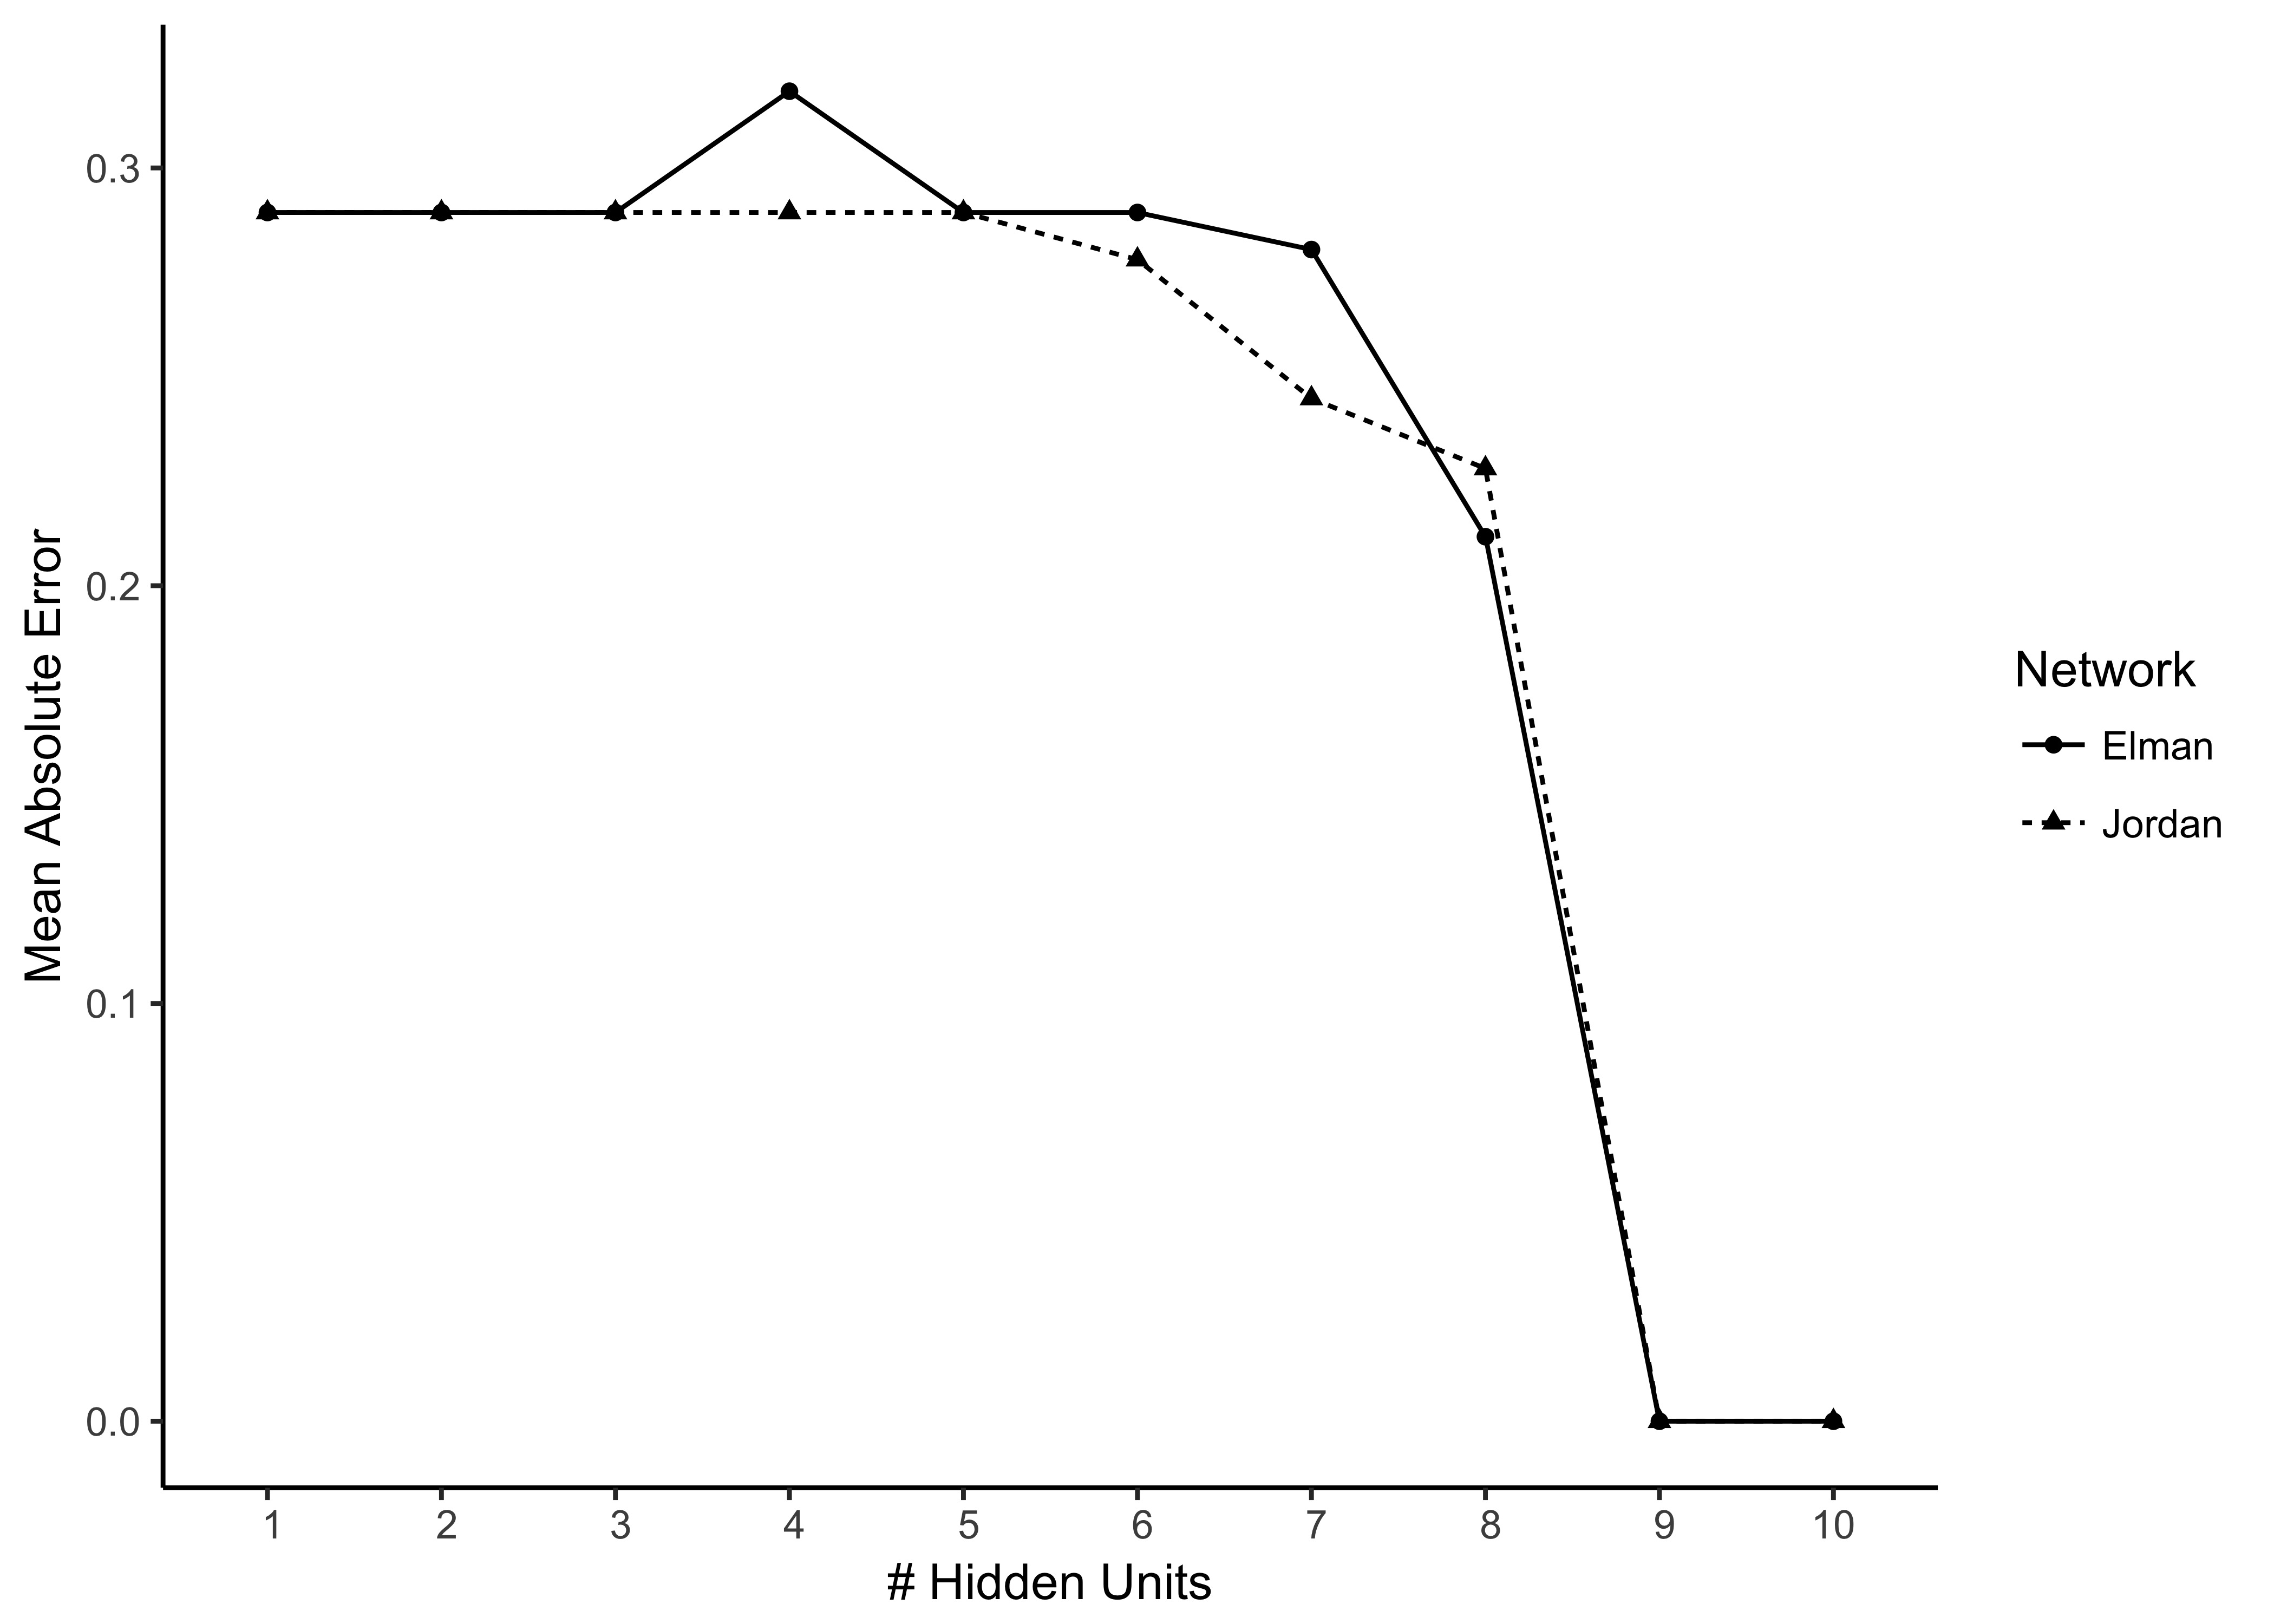
\includegraphics[width=1.0\textwidth]{figures/error_nc_4}
	\caption{Results of an experiment to define the appropriated number of hidden units in a recurrent network to generate non-complementary candidates explanations for the program $\CalP_{sup}$. The size of the hidden units vary from one to ten. The graph plots the mean absolute error (MAE) for a 10-fold cross-validation averaged over ten trials for each network configuration.}
	\label{fig:error_nc_4}
\end{figure}

With this we can conclude that both a Jordan and an Elman network constructed in the way described above have one hundred percent of accuracy for the task of generating all the possible non-complementary candidate explanations for the program $\CalP_{sup}$ and its respective set of abducibles $\CalA_{\CalP_{sup}}$. Although we have focused on showing the results for the set of abducibles $\CalA_{\CalP_{sup}}$, it is easy to observe that the experiment can be repeated in the exact same way for any set of abducible which has cardinality four. The only difference is on which abducible each of the four bits represent which in our case was $e^\top$, $e^\top$, $e^\top$, and $e^\top$, but the representation can easily be substituted by any other set of abducibles without affecting the procedure.

Moreover, as it is shown in the algorithms presented earlier, the process is specified in an abstract level such that it should work for a given set of abducibles of any size. Therefore, we would like to abstract from the previous example and show how one could follow the same steps for any other program with corresponding set of abducibles of different sizes. For this purpose, consider an arbitrary program $\CalP$ and its corresponding set of abducibles $\CalA_\CalP$, where |$\CalA_\CalP$| = N. Both the input and output layers would consist of N+1 units. As explained previously, the ideal number of hidden units can vary from case to case and one way to define this if by reproducing the same experiment developed above. Both the Jordan and Elman networks can be structured in the same way, with the difference on the recurrent connections only.

To show that this is indeed the case we will reproduce the experiment and analyse its output for other values of N. In order to do so, we will show example of programs which have a respective size of abducibles of size N. However, note that, just as we have explained earlier, the programs are only for illustrative purpose but the results shown here can be generalised for any set of abducibles of corresponding cardinality~N. Consider the variations of program $\CalP_{sup}$ shown in Example~\ref{example:suppressionvariation} on page~\pageref{example:suppressionvariation}.

A network that sequentially generates the candidate explanations in $\CalC_{\CalA_{\CalP_{sup'}}}$ consists of three input units and three output units. In order to define the adequate number of units in the hidden layer, we reproduce the experiment for Jordan and Elman networks now following the configurations described here. As it is shown in Figure~\ref{fig:error_nc_2}, again the Jordan and the Elman networks have presented a similar behaviour and a hidden layer consisting of four units seems to be the most adequate for both types of networks. For the candidate explanations $\CalC_{\CalA_{\CalP_{sup''}}}$, the network consists of seven input units and seven output units. Regarding the hidden units, as it is shown in Figure~\ref{fig:error_nc_6}, the Jordan and Elman networks need thirteen and fourteen hidden units, respectively. This last case is also a strong indication on the generalisation capacity of such networks, since there are twenty-seven candidate explanations and less than the half of this number is needed in hidden units.

With this we can conclude that creating Jordan and Elman networks for the generation on non-complementary candidate explanations can be done for sets of abducibles of different sizes by following the steps defined in this section. Moreover, the experiment to define which of the two networks is more suitable and which is the most adequate number of hidden units can also easily be reproduced for the different sets of abducibles. 

\vspace*{\fill}
\begin{tcolorbox}
\begin{example}
\label{example:suppressionvariation}
\normalfont 
Consider a subset $\CalP_{sup'}$ of the program $\CalP_{sup}$ only consisting of the following two clauses:
\[
\begin{array}{lclclcl}
l &\leftarrow& e \wedge \neg ab_1. &\quad\quad& ab_1 &\leftarrow& \bot.
\end{array}
\]
The repesctive set of abducibles $\CalA_{\CalP_{sup'}}$ consists of the following fact and assumption:
\[
\begin{array}{lclclcl}
e &\leftarrow& \top. &\quad\quad& e &\leftarrow& \bot.
\end{array}
\]
The set of non-complementary candidate explanations $\CalC_{\CalA_{\CalP_{sup'}}}$ consists of the following three elements:
\[
\begin{array}{lclclclclcl}
\CalC_0 &=& \emptyset, &\quad& \CalC_1 &=& \{e \leftarrow \top\}, &\quad& \CalC_2 &=& \{e \leftarrow \bot\}.
\end{array}
\]

Consider a program $\CalP_{sub''}$ which is the program $\CalP_{sup}$ with an additional clause, e.g. \textit{if she has a presentation to prepare, then she will study late in the library}. Thus, we have the program $\CalP_{sub''}$ consisting of all the four clauses in $\CalP_{sup}$ plus the following two:
\[
\begin{array}{lclclcl}
l &\leftarrow& p \wedge \neg ab_3. &\quad& ab_3 &\leftarrow& \bot.\\
\end{array}
\]
Where the new atom $p$ stands for \textit{she has a presentation to prepare} and $ab_3$ for the abnormality, as usual. Its repesctive set of abducibles $\CalA_{\CalP_{sup''}}$ consists of the following six elements:
\[
\begin{array}{ccccc}
e \leftarrow \top. & \quad & t \leftarrow \top. & \quad & p \leftarrow \top. \\
e \leftarrow \bot. & \quad & t \leftarrow \bot  & \quad & p \leftarrow \bot.
\end{array}
\]

The set of non-complementary candidate explanations $\CalC_{\CalA_{\CalP_{sup''}}}$ consists of the following twenty seven elements:
\[
\begin{array}{lclclcl}
\CalC_1&=&\emptyset, &&&& \\
\CalC_2 &=& \{e \leftarrow \top\}, && \CalC_3 &=& \{e \leftarrow \bot\}, \\
\CalC_4 &=& \{t \leftarrow \top\}, && \CalC_5 &=& \{t \leftarrow \bot\}, \\
\CalC_6 &=& \{p \leftarrow \top\}, && \CalC_7 &=& \{p \leftarrow \bot\}, \\
\CalC_8 &=& \{e \leftarrow \top, t \leftarrow \top\}, && \CalC_9 &=& \{e \leftarrow \top, t \leftarrow \bot\}, \\
\CalC_{12} &=& \{e \leftarrow \bot, t \leftarrow \top\}, && \CalC_{13} &=& \{e \leftarrow \bot, t \leftarrow \bot\}, \\
 \CalC_{14} &=& \{e \leftarrow \bot, p \leftarrow \top\}, && \CalC_{15} &=& \{e \leftarrow \bot, p \leftarrow \bot\}, \\
\CalC_{16} &=& \{t \leftarrow \top, p \leftarrow \top\}, && \CalC_{17} &=& \{t \leftarrow \top, p \leftarrow \bot\}, \\
\CalC_{18} &=& \{t \leftarrow \bot, p \leftarrow \top\}, && \CalC_{19} &=& \{t \leftarrow \bot, p \leftarrow \bot\}, \\
\CalC_{20} &=& \{e \leftarrow \top, t \leftarrow \top, p \leftarrow \top\}, && \CalC_{21} &=& \{e \leftarrow \top, t \leftarrow \top, p \leftarrow \bot\}, \\
\CalC_{22} &=& \{e \leftarrow \top, t \leftarrow \bot, p \leftarrow \top\}, && \CalC_{23} &=& \{e \leftarrow \top, t \leftarrow \bot, p \leftarrow \bot\}, \\	     
\CalC_{24} &=& \{e \leftarrow \bot, t \leftarrow \top, p \leftarrow \top\}, && \CalC_{25} &=& \{e \leftarrow \bot, t \leftarrow \top, p \leftarrow \bot\}, \\	
\CalC_{26} &=& \{e \leftarrow \bot, t \leftarrow \bot, p \leftarrow \top\}, && \CalC_{27} &=& \{e \leftarrow \bot, t \leftarrow \bot, p \leftarrow \bot\}. 	
\end{array}
\]
\end{example}
\end{tcolorbox}
\vspace*{\fill}

\begin{figure}
	\centering
	\begin{subfigure}[b]{1.\textwidth}
	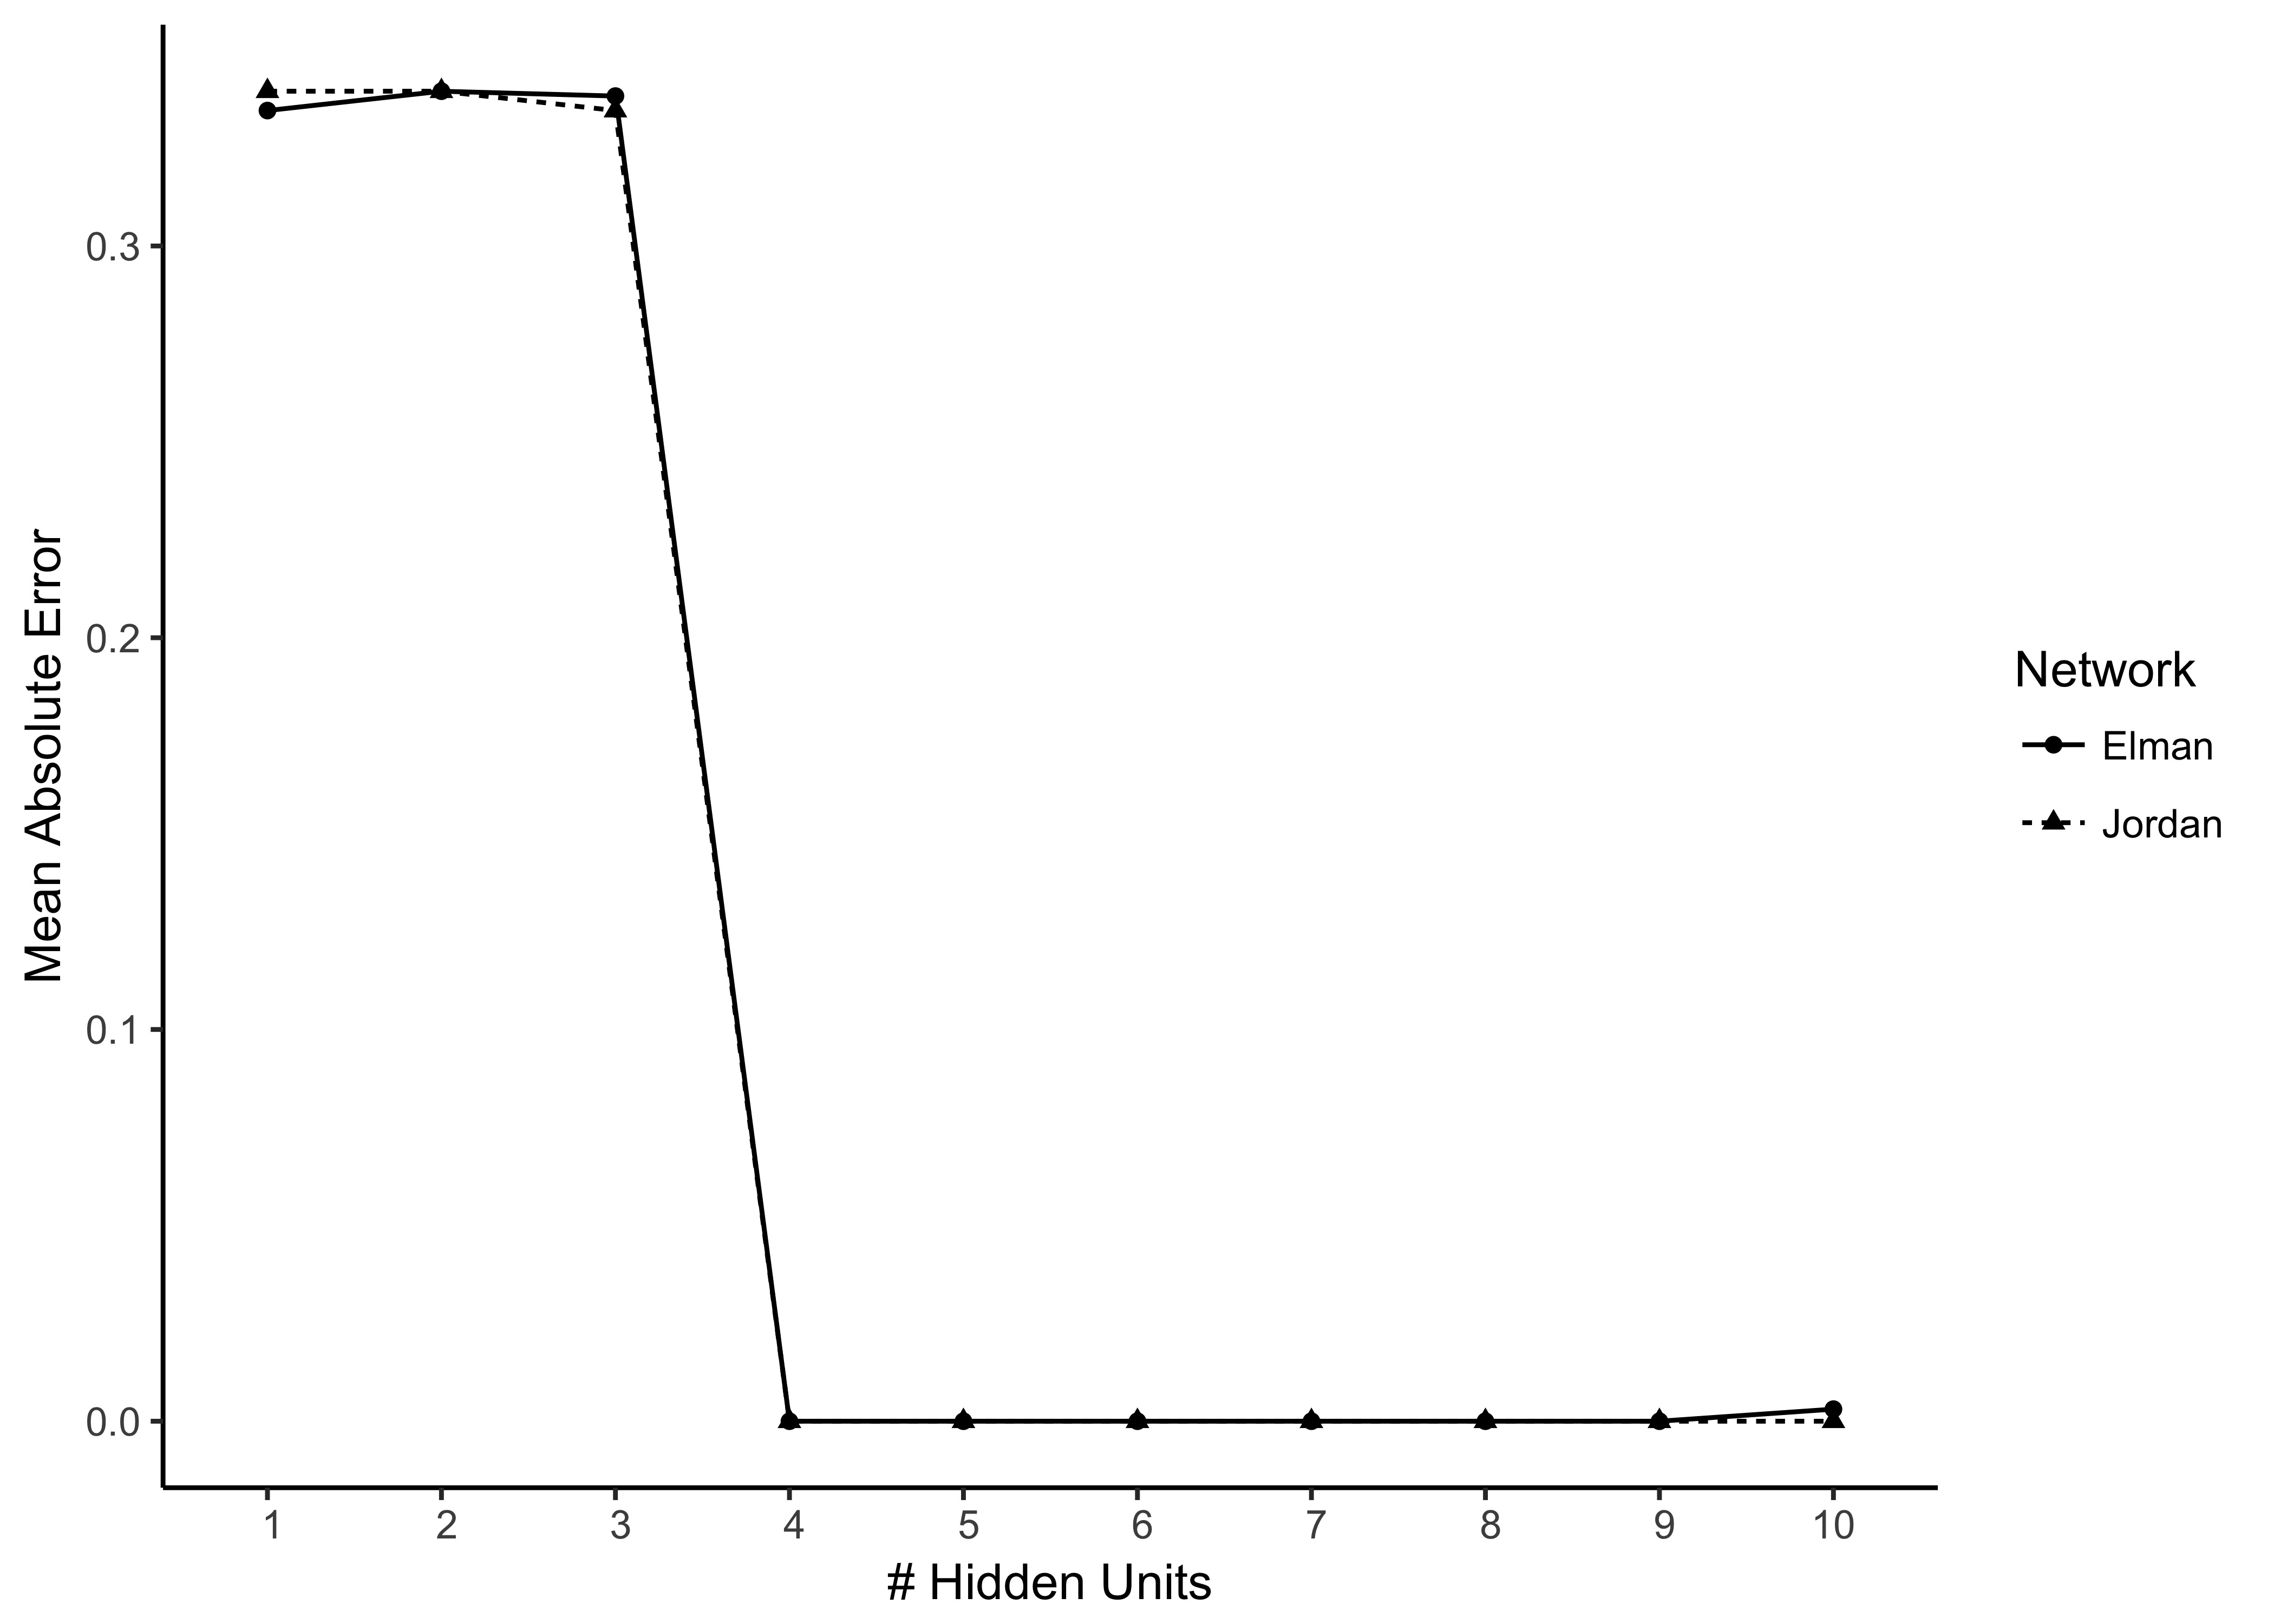
\includegraphics[width=0.9\textwidth]{figures/error_nc_2}
	\caption{Set of abducibles of cardinality two.}
	\label{fig:error_nc_2}
	\end{subfigure}
	\bigskip
	\begin{subfigure}[b]{1.0\textwidth}
  	 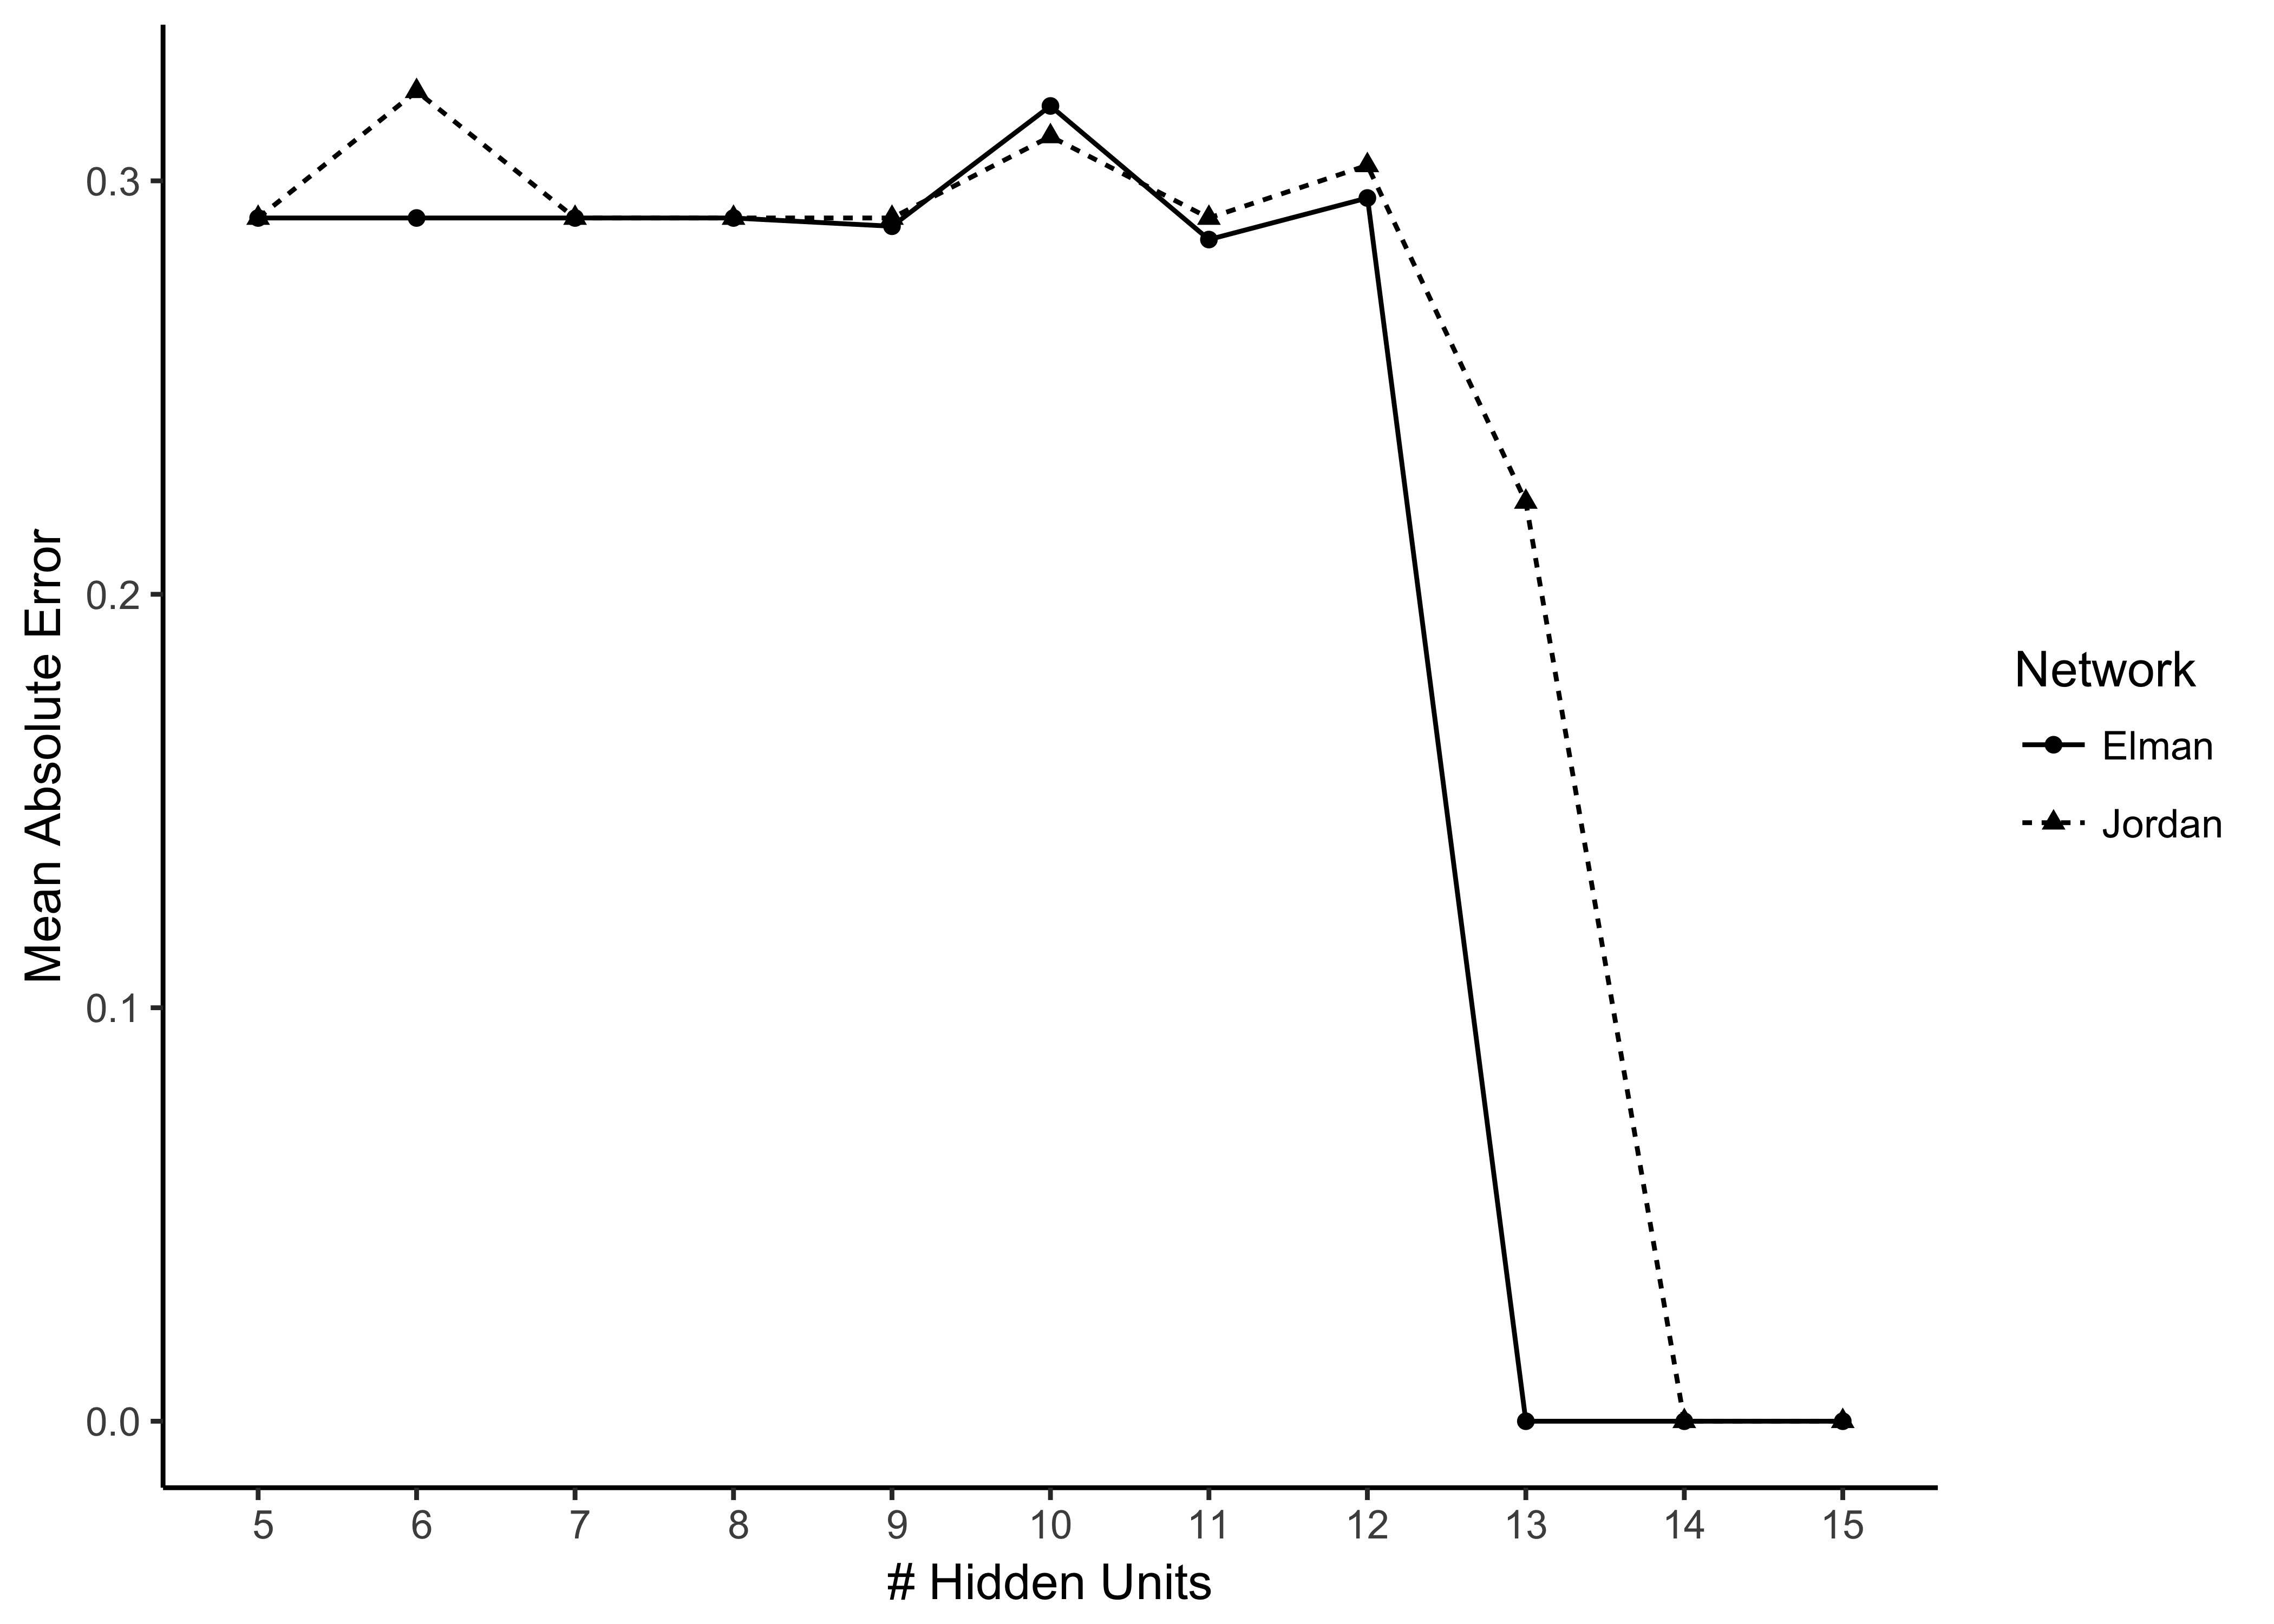
\includegraphics[width=0.9\textwidth]{figures/error_nc_6}
	 \caption{Set of abducibles of cardinality six.}
	\label{fig:error_nc_6}
	\end{subfigure}
	\caption{Results of an experiment to define the appropriated number of hidden units in a recurrent network to generate non-complementary candidates explanations for a given set of abducibles with cardinality two (a) and six (b). The size of the hidden units vary from one to ten. The graph plots the mean absolute error (MAE) for a 10-fold cross-validation averaged over ten trials for each network configuration.}
\end{figure}

Remember that for a set of abducibles $\CalA_\CalP$ of cardinality $2n$, there are $3^n$ non-complementary candidate explanations $\CalC_{\CalA_\CalP}$. These $3^n$ candidates can be ordered as $3^n!$ different sequences. For example, in the most basic case which is $n = 1$, we have that cardinality of $\CalA_\CalP$ is two, there are three candidate explanation which can be ordered in six different sequences, i.e.
\[
\begin{array}{lclclcl}
\CalC_{\CalA_\CalP}^1 &=& \{\CalC_1, \CalC_2, \CalC_3\}, &\quad& \CalC_{\CalA_\CalP}^2 &=& \{\CalC_1, \CalC_3, \CalC_2\},\\
\CalC_{\CalA_\CalP}^3 &=& \{\CalC_2, \CalC_3, \CalC_1\}, &\quad& \CalC_{\CalA_\CalP}^4 &=& \{\CalC_2, \CalC_1, \CalC_3\},\\
\CalC_{\CalA_\CalP}^5 &=& \{\CalC_3, \CalC_1, \CalC_2\}, &\quad& \CalC_{\CalA_\CalP}^6 &=& \{\CalC_3, \CalC_2, \CalC_1\}.
\end{array}
\]

Similarly, there are several different sequences for the sets of non-complementary candidate explanations regarding different cardinalities of the abducibles. In order to train the network with this different orders, we only have to set up the parameter \textit{candidates} in the algorithms shown earlier and everything else works in the same way.

For instance, when solving Byrne's selection task represented by $\CalP_{sup}$, we have used the same sequence from Chapter~\ref{sec:cn} for sake of simplicity. However, any other sequence could have been used, e.g.
\[
\begin{array}{lcl}
candidates^1 &=& \{00000, 10100, 10000, 01000, 00100, 00010, 10010, 01100, 01011\}, \\
candidates^2 &=& \{00000, 10100, 01011, 10000, 01000, 00100, 00010, 10010, 01100\}, \\
candidates^3 &=& \{00000, 10100, 10010, 10000, 01000, 00100, 00010, 01100, 01011\},  \\
candidates^4 &=& \{00000, 00100, 10010, 10000, 01000, 10100, 00010, 01100, 01011\},  \\
\dots\\
candidates^{9!} &=& \{00100, 00010, 01100, 01011, 10100, 10010, 10000, 01000, 00000\}. 
\end{array}
\]

This shows that not only the same result as the one from the previous approach can be archived, but also that arbitrary sequences can be easily considered. However, as explained before, generating the non-complementary candidate explanations is not our main goal. Thus, we will now show how the same networks can also be used to generate the minimal candidate explanations.


\section{Minimal Candidate Explanations}
\label{sec:nn:mce}

In this section will show that recurrent networks can be used not only to generate the non-complementary candidate explanations, as shown in Section~\ref{sec:nn:ncce}, but also to generate the minimal candidate explanations for a given observation. The most important information necessary for this modification is whether the last candidate explanation has in fact explained the given observation or not.  

We again show that this is indeed the case by means of an example. Thus, reconsider the program $\CalP_{sup}$ from Example~\ref{example:suppression} on page~\pageref{example:suppression}. The only necessary modification in the structure of the Jordan and Elman networks presented in Section~\ref{sec:nn:ncce} is to add one bit in the input vector which will now consist of six bits instead of five. This new bit gives us the informations of whether the last candidate was an explanation or not. This is reflected in the network by an additional unit in the input layer. The new version of both networks is shown in Figure~\ref{fig:rnnmin}.

The activation of this new unit $e$ (\textit{explanation}) is done by the external network responsible for checking whether a candidate explanation has explained the given observation or not. This is the same network which activates the unit \textit{next} (\textit{next}), which means that the request of a new candidate explanation and the activation of unit $e$ are synchronised.

\begin{figure}
\centering
   \begin{subfigure}[b]{0.55\textwidth}
   \scalebox{0.7}{\jordanmin}
   \caption{Jordan Network.}
   \bigskip
\end{subfigure}
\begin{subfigure}[b]{0.55\textwidth}
   \scalebox{0.7}{\elmanmin}
   \caption{Elman Network.}
\end{subfigure}
\caption{Structure of the Jordan (a) and Elman (b) networks for the generation of all non-complementary candidate explanations for the program $\CalP_{sup}$. Solid lines are trainable.}
\label{fig:rnnmin}
\end{figure}

Also reconsider the observation 
\[
\CalO_1 = \{l\},
\] 
we know that its minimal explanations given program $\CalP_{sup}$ and the observation $\CalO_1$ are the following:
\[
\begin{array}{lcl}
\CalE_1 &=& \{e \leftarrow \top\}, \\
\CalE_2 &=& \{t \leftarrow \top\}.
\end{array}
\]
Thus, when generating the candidate explanations, all the supersets of the two explanations $\CalE_1$ and $\CalE_2$ should not be taken into account. Thus, if we are also considering that the candidate explanations will be generated following the same order as in the previous sections, the following candidates explanations are expected to be generated: 
\[
\begin{array}{lcl}
\CalE_0 &=& \emptyset,\\
\CalE_1 &=& \{e \leftarrow \top\}, \\
\CalE_2 &=& \{e \leftarrow \bot\}, \\
\CalE_3 &=& \{t \leftarrow \top\}, \\
\CalE_4 &=& \{t \leftarrow \bot\}, \\
\CalE_8 &=& \{e \leftarrow \bot, t \leftarrow \bot\}. 
\end{array}
\]

In terms of the 5-bit binary vectors corresponding to the expected output the expected sequence if we have the next unit activated for six time steps in a row would be: 
\[
00000, 10000, 01000, 00100, 00010, 01011. 
\]
But of course, just as we had before, this is not always the case and, depending on the activation of the next unit, any sequence of the following form would be valid: 
\[
(00000)^+, (10000)^+, (01000)^+, (00100)^+, (00010)^+, (01011)^+.
\]
All possible inputs and its respective expected outputs for this example is shown in Table~\ref{table:inoutmin}. 

\begin{table}
	\centering
	\begin{subtable}[h]{0.30\textwidth}
		\centering
		\begin{tabular}{cc}
		Input & Output \\
		\hline
		000000 & 00000 \\
		100001 & 10000 \\
		010000 & 01000 \\
		001001 & 00100 \\
		000100 & 00010 \\
		010100 & 01011 \\
		\end{tabular}
		\bigskip
		\caption{Cases where the fifth bit in the input is \textit{zero}}
		\label{table:trainingexplanations:zero}
	\end{subtable}
	\hspace{3cm}
	\begin{subtable}[h]{0.30\textwidth}
		\centering
		\begin{tabular}{cc}
		Input & Output \\
		\hline
		000010 & 10000 \\
		100011 & 01000 \\
		010010 & 00100 \\
		001011 & 00010 \\
		000110 & 01011 \\
		010110 & 00000 \\
		\end{tabular}
		\bigskip
		\caption{Cases where the fifth bit in the input is \textit{one}}
		\label{table:trainingexplanations:one}
	\end{subtable}
	\caption{Each possible input and its respective expected output for the generation of minimal candidate explanations for the program $\CalP_{sup}$ and observation $\CalO_1 = \{l\}$ considering a specific ordering.}
	\label{table:inoutmin}
\end{table}

Note that, when we assume the candidates to be minimal, there is a cardinality constraint implicit in the ordering of the candidates. For the program $\CalP_{sup}$ which we are discussing, for example, the following ordering could no longer be considered: 
\[
\begin{array}{lcl}
candidates^2 &=& \{00000, 10100, 01011, 10000, 01000, 00100, 00010, 10010, 01100\}.
\end{array}
\]
The candidate explanation $10100$ representing $\{e^\top, t^\top\}$ is a positive non-minimal candidate explanation which the generation could not have been avoided if this order is considered. Therefore, we assume that for the generation of minimal candidate explanations, the sequences will respect the cardinality order. However, this does not mean that the order is now fixed. For a given set of candidates $\CalC$, there are the following number of sequences respecting the cardinality constraint:
\[
c_0! * c_1! * \dots * c_n!
\]
where $c_i$ represents the number of candidates in $\CalC$ with cardinality $i$. In our example, the six minimal candidates can be ordered as
\[
1!*4!*1! = 16
\]
different sequences, as there is one candidate with cardinality zero, four with cardinality one and one with cardinality two.

The training and the testing phase of the Jordan and Elman networks are done in the same way as described before. The only difference now is in the input of the network and the training and testing data. The input of the network will now contain an aditonal bit representing the request of next candidate explanation. The data will now be generated considering all the possibilities of candidates being explanations and the resulting minimal set of candidate explanations for each of this cases. Table~\ref{table:inoutmin} shows one of this potential cases for a given program having a correspondent set of abducibles of size four.

As we know that in the case where the fifth bit is zero only the identity function is computed, we will only consider the cases where the fifth bit is one to demonstrate all the possible sixteen sequences for potential programs $\CalP$ and observations $\CalO$, such that the set of abducibles $\CalA_\CalP$ has cardinality four. Figure~\ref{fig:exptree} on page~\pageref{fig:exptree} shows all the possible outcomes and paths for each of these cases and Table~\ref{table:allinoutmin} shows the data we use in the training process such that the Jordan and Elman networks can reflect this behaviour.

So the new training and testing data for a given program $\CalP$ with a respective set of abducibles $\CalA_\CalP$ of size four will not only have a fixed sequence of size nine being generated, but all the ten different sequences of different sizes. This different sequences are due to the possible variations in the activation of unit $e$. We assume a corresponding program and observation which which leads to these expected data can be easily found. Therefore, in each pass of the training phase as well as in the testing phase, we choose one arbitrary mapping of potential input to expected output from the sixteen shown in Table~\ref{table:allinoutmin} on page~\pageref{table:allinoutmin}.

\begin{table}
	\begin{subtable}[h]{0.10\textwidth}
		\centering
		\begin{tabular}{cc}
		Input & Output \\
		\hline
		000010	&	10000 \\
		100010	&	01000 \\
		010010	&	00100 \\
		001010	&	00010 \\
		000110	&	10100 \\
		1010	10	&	10010 \\
		100110	&	01100 \\
		011010	&	01011 \\
		010110	&	00000 \\
		\end{tabular}
		\bigskip
		%\caption{}
		\label{table:trainingexplanations:zero}
	\end{subtable}
	\hspace{3.75cm}
	\begin{subtable}[h]{0.10\textwidth}
		\centering
		\begin{tabular}{cc}
		Input & Output \\
		\hline
		010110	&	00000\\
		000010	&	10000\\
		100011	&	01000\\
		010010	&	00100\\
		001010	&	00010\\
		000110	&	01100\\
		011010	&	01011\\
		&\\
		&\\
		\end{tabular}
		\bigskip
		%\caption{Cases where the fifth bit in the input is \textit{one}}
		\label{table:trainingexplanations:one}
	\end{subtable}
	\hspace{3.75cm}
	\begin{subtable}[h]{0.10\textwidth}
		\centering
		\begin{tabular}{cc}
		Input & Output \\
		\hline
		100110	&	00000\\
		000010	&	10000\\
		100010	&	01000\\
		010011	&	00100\\
		001010	&	00010\\
		000110	&	10100\\
		1010	10	&	10011\\
		&\\
		&\\
		\end{tabular}
		\bigskip
		%\caption{Cases where the fifth bit in the input is \textit{one}}
		\label{table:trainingexplanations:one}
	\end{subtable}
	\newline
	\begin{subtable}[h]{0.10\textwidth}
		\centering
		\begin{tabular}{cc}
		Input & Output \\
		\hline
		010110	&	00000\\
		000010	&	10000\\
		100010	&	01000\\
		010010	&	00100\\
		001011	&	00010\\
		000110	&	10010\\
		100110	&	01011\\
		\end{tabular}
		\bigskip
		%\caption{Cases where the fifth bit in the input is \textit{one}}
		\label{table:trainingexplanations:one}
	\end{subtable}
	\hspace{3.75cm}
	\begin{subtable}[h]{0.10\textwidth}
		\centering
		\begin{tabular}{cc}
		Input & Output \\
		\hline
		011010	&	00000\\
		000010	&	10000\\
		100010	&	01000\\
		010010	&	00100\\
		001010	&	00010\\
		000111	&	10100\\
		1010	10	&	01101\\
		\end{tabular}
		\bigskip
		%\caption{Cases where the fifth bit in the input is \textit{one}}
		\label{table:trainingexplanations:one}
	\end{subtable}
	\hspace{3.75cm}
	\begin{subtable}[h]{0.10\textwidth}
		\centering
		\begin{tabular}{cc}
		Input & Output \\
		\hline
		010110	&	00000\\
		000010	&	10000\\
		100011	&	01000\\
		010010	&	00100\\
		001011	&	00010\\
		000110	&	01011\\
		\end{tabular}
		\bigskip
		%\caption{Cases where the fifth bit in the input is \textit{one}}
		\label{table:trainingexplanations:one}
	\end{subtable}
	\newline
	\begin{subtable}[h]{0.10\textwidth}
		\centering
		\begin{tabular}{cc}
		Input & Output \\
		\hline
		011010	&	00000\\
		000010	&	10000\\
		100011	&	01000\\
		010010	&	00100\\
		001010	&	00010\\
		000111	&	01101\\
		\end{tabular}
		\bigskip
		%\caption{Cases where the fifth bit in the input is \textit{one}}
		\label{table:trainingexplanations:one}
	\end{subtable}
		\hspace{3.75cm}
		\begin{subtable}[h]{0.10\textwidth}
		\centering
		\begin{tabular}{cc}
		Input & Output \\
		\hline
		100110	&	00000\\
		000010	&	10000\\
		100010	&	01000\\
		010011	&	00100\\
		001011	&	00010\\
		000110	&	10011\\
		\end{tabular}
		\bigskip
		%\caption{Cases where the fifth bit in the input is \textit{one}}
		\label{table:trainingexplanations:one}
	\end{subtable}
	\hspace{3.75cm}
	\begin{subtable}[h]{0.10\textwidth}
		\centering
		\begin{tabular}{cc}
		Input & Output \\
		\hline
		010110	&	00000\\
		000010	&	10000\\
		100010	&	01000\\
		010011	&	00100\\
		001010	&	00010\\
		000111	&	01011\\
		\end{tabular}
		\bigskip
		%\caption{Cases where the fifth bit in the input is \textit{one}}
		\label{table:trainingexplanations:one}
	\end{subtable}
	\newline
	\begin{subtable}[h]{0.2\textwidth}
		\centering
		\begin{tabular}{c|c}
		Input & Output \\
		\hline
		000111	\quad	000111	\quad	000111	\quad	000111	\quad	000111	\quad	000110	\quad	000110    &	00000\\	
		000010	\quad	000010	\quad	000010	\quad	000010	\quad	000010	\quad	000010	\quad	000010	&	10000\\
		100011	\quad	100010	\quad	100010	\quad	100011	\quad	100011	\quad	100011	\quad	100011	&	01000\\
		010011	\quad	010010	\quad	010011	\quad	010010	\quad	010011	\quad	010011	\quad	010011	&	00100\\
		001011	\quad	001011	\quad	001011	\quad	001011	\quad	001010	\quad	001011	\quad	001010	&	00011\\
		\end{tabular}
		\bigskip
		%\caption{Cases where the fifth bit in the input is \textit{one}}
		\label{table:trainingexplanations:one}
	\end{subtable}
	\caption{Input and expected output for all the sixteen possible combinations of the fifth bit representing $explanation$.}
	\label{table:allinoutmin}
\end{table}

The same experiment described in the previous section is then performed again, but now taking into account the modifications in the generation of the training and verification data. In practice, all the algorithms shown before work exactly in the same way with the only difference that instead of having one fixed sequence of candidate explantions to be learned, we now have a set of possible candidate explanations. An arbitrary one is chosen from this set in the beginning of every new training phase.

The performance measure considered is also the same, e.g. mean absolute error. Figure~\ref{fig:error_min_4} on page~\pageref{fig:error_min_4} shows the result of this experiment for the generation of minimal candidate explanation for a given program $\CalP$ with set of abducibles $\CalA_\CalP$ of size four. This network could then be used, for instance, to generate the minimal candidate explanations for a given observation $\CalO$ given the program~$\CalP_{sup}$, since its respective set of abducibles $\CalA_{\CalP_{sup}}$ consists of four facts and assumptions.

If we filter the results shown in Figure~\ref{fig:error_min_4} to see only the mean absolute error with respect to the cases shown in Table~\ref{table:inoutmin} which corresponds to the given observation $\CalO_1$, we get the results shown in Figure~\ref{fig:l_error_min_4} on page~\ref{fig:error_min_4}.

\begin{figure}
	\centering
	\begin{subfigure}[b]{1.\textwidth}
	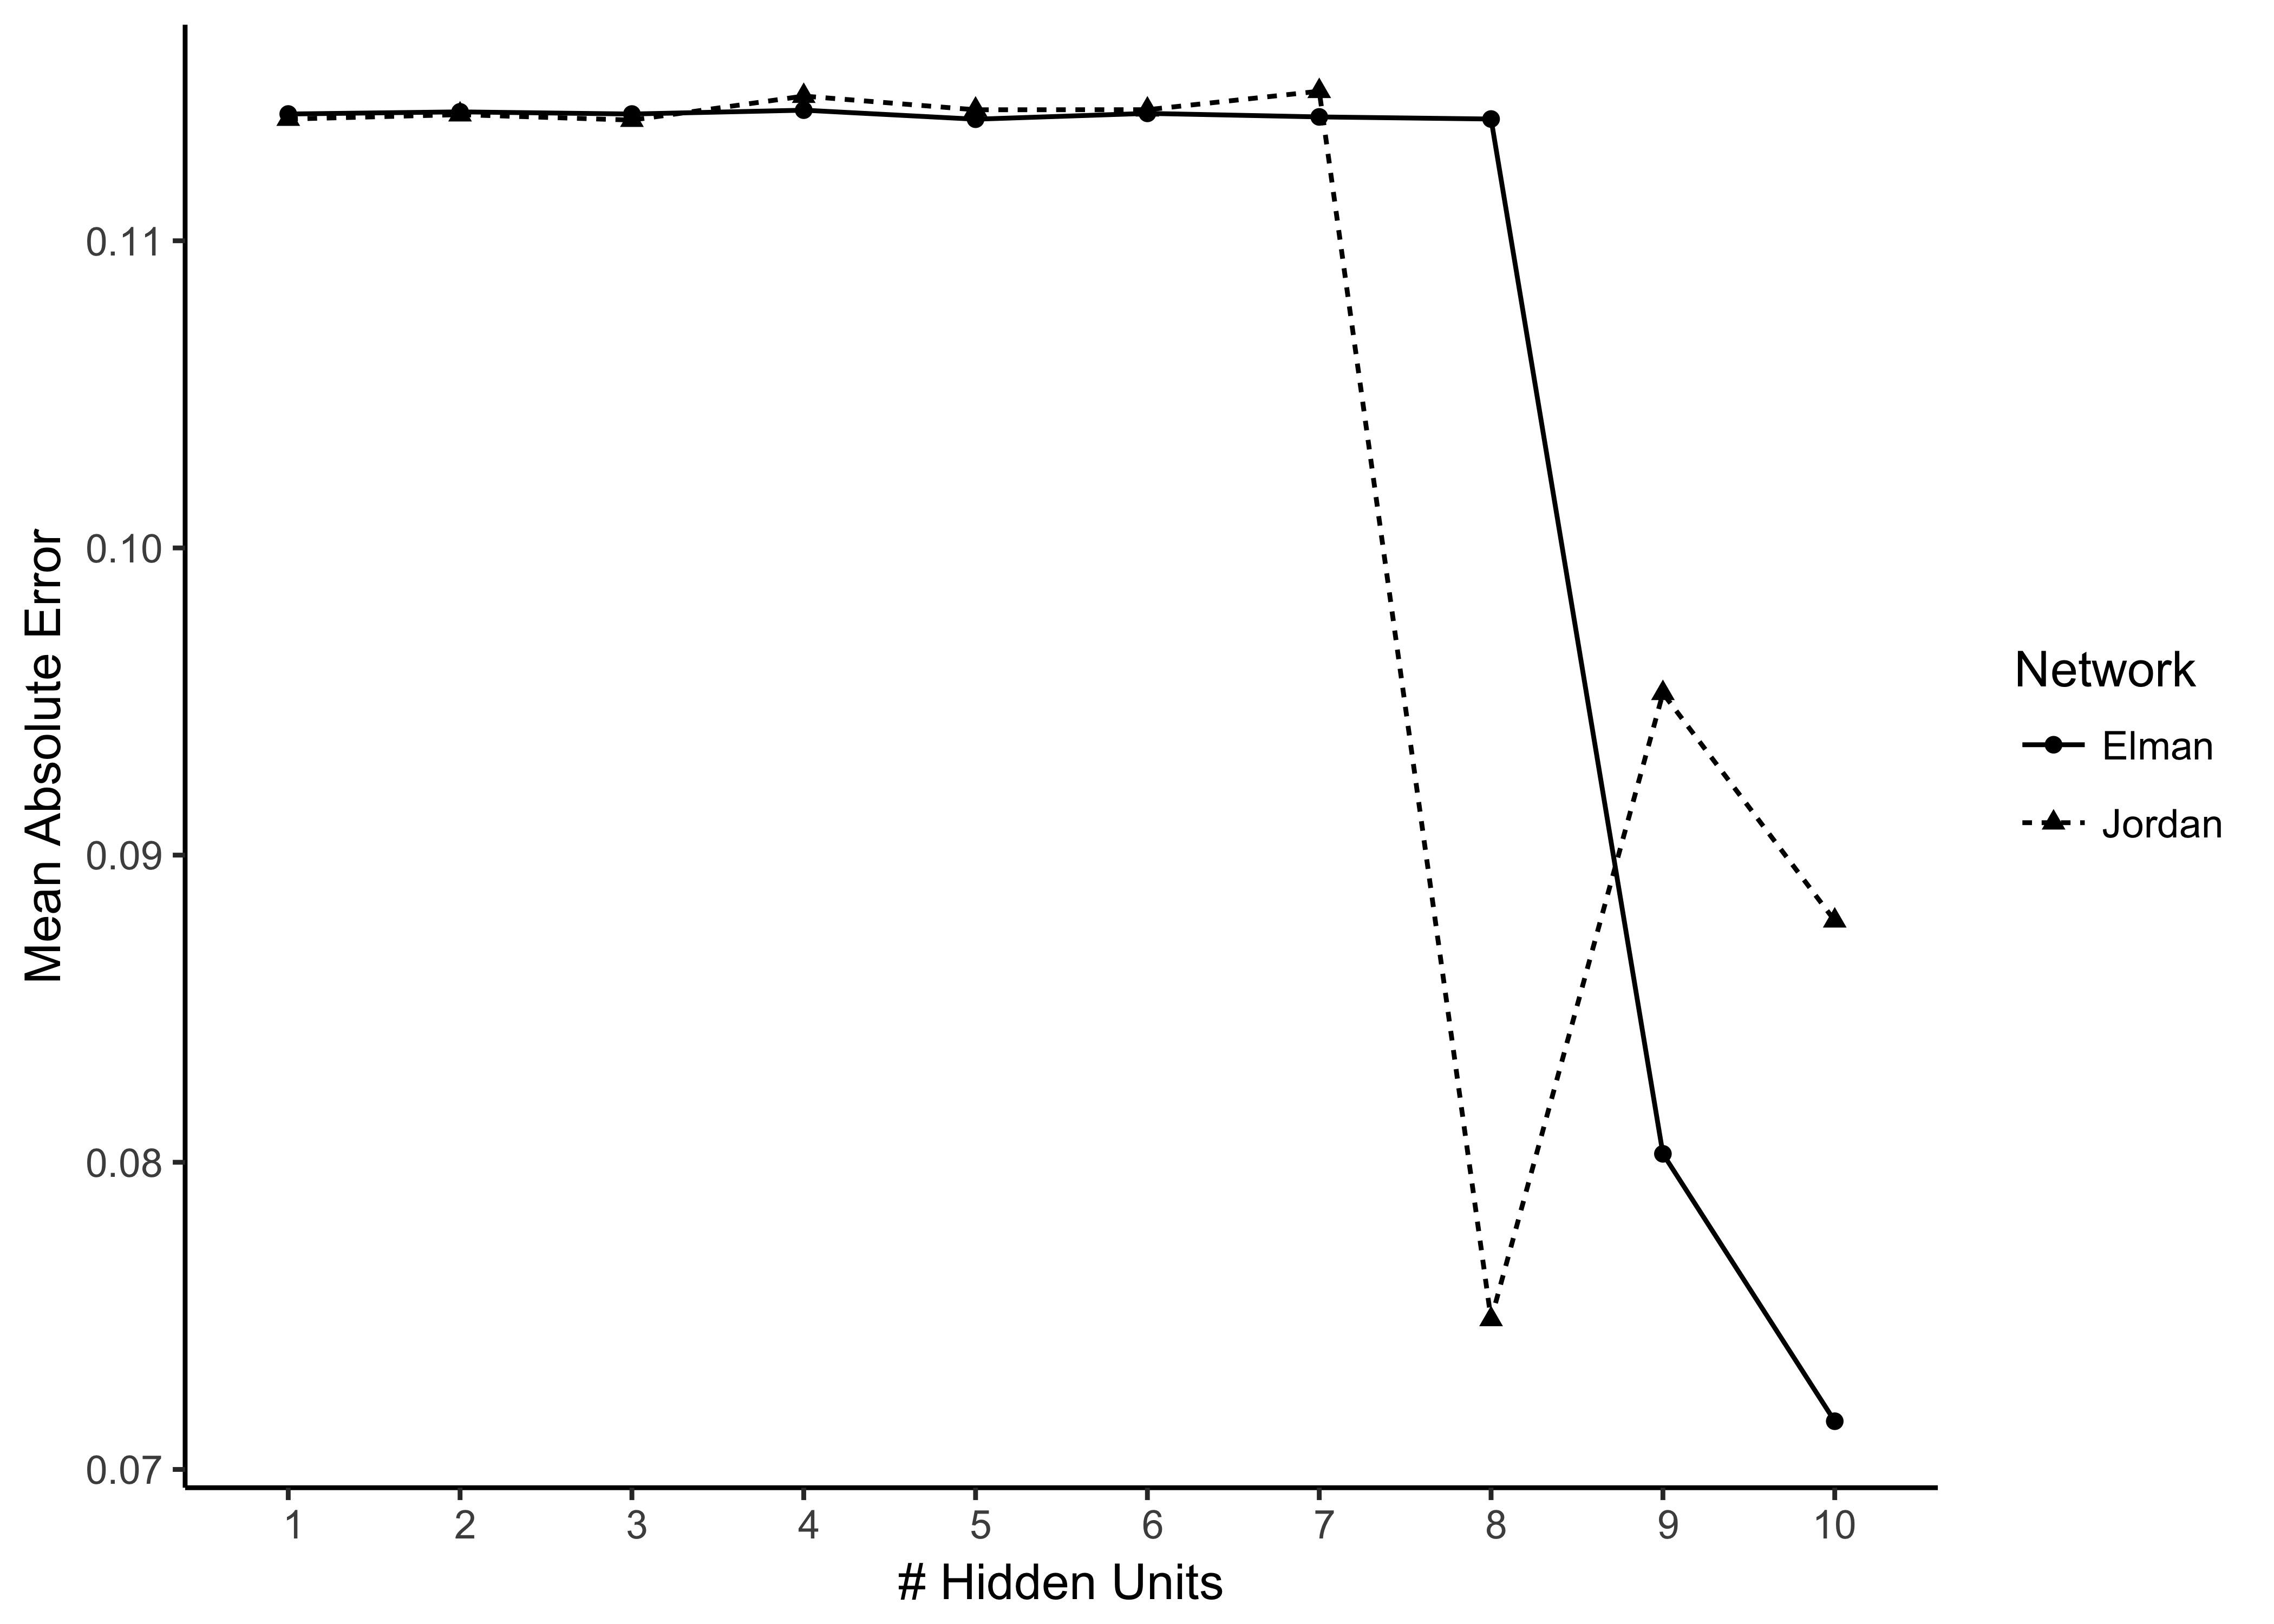
\includegraphics[width=0.9\textwidth]{figures/error_min_4}
	\caption{General results.}
	\label{fig:error_min_4}
	\end{subfigure}
	\bigskip
	\begin{subfigure}[b]{0.9\textwidth}
  	 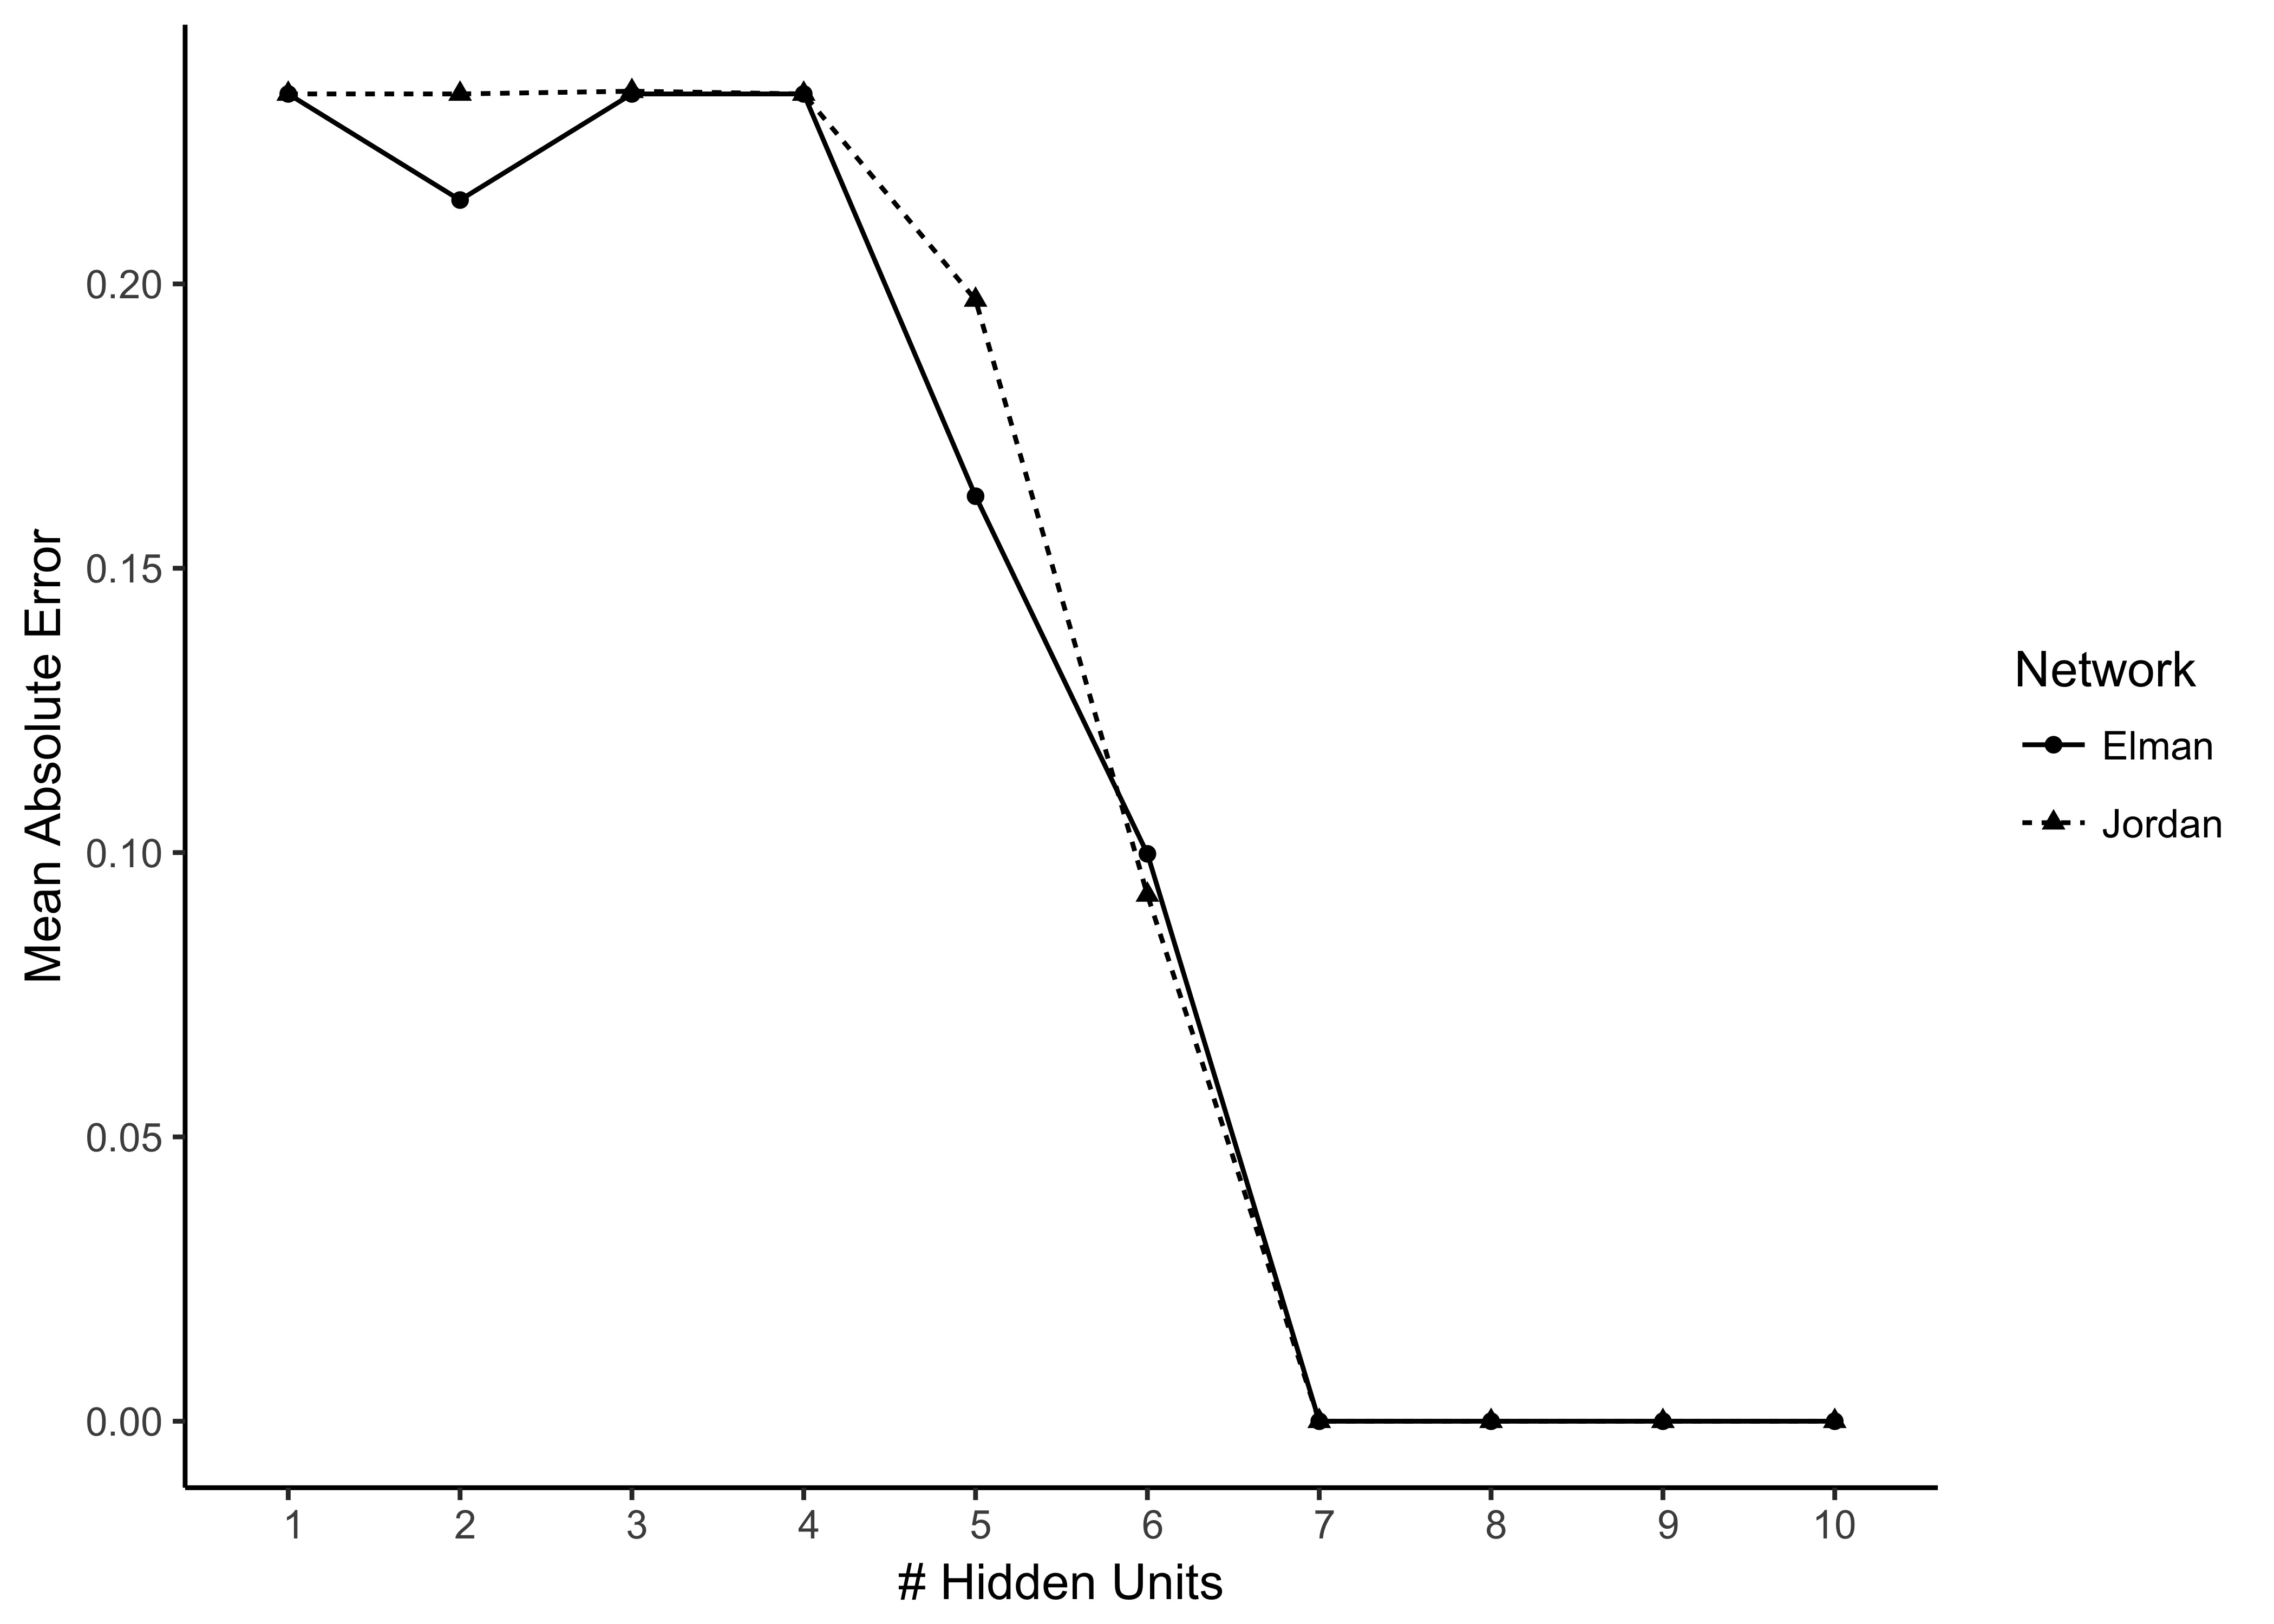
\includegraphics[width=1.0\textwidth]{figures/l_error_min_4}
	 \caption{Results filtrated by the test cases considering program $\CalP_{sup}$ and observation~$\CalO_1$.}
	\label{fig:l_error_min_4}
	\end{subfigure}
	\caption{Results of an experiment to define the appropriated number of hidden units in a recurrent network to generate non-complementary candidates explanations for a set of abducibles of cardinality four, considering arbitrary programs and potential explanations. The size of the hidden units vary from one to ten. The graph plots the mean absolute error (MAE) for a 10-fold cross-validation averaged over ten trials for each network configuration.}
\end{figure}

With this we have shown that the Jordan and Elman networks can also be used to generate only the minimal candidate explanations for observation $\CalO_1$ given program $\CalP_{sup}$ with accuracy of one hundred percent starting from seven hidden units on. 

Let us now consider another observation, e.g.
\[
\CalO_2 = \{\neg l\}
\]
In this case, the only explanation for the observation $\CalO_2$ given the program $\CalP_{sup}$ would be the explanation
\[
\CalE_9 = \{e \leftarrow \bot, t \leftarrow \bot\}.
\]

Therefore, all the nine candidate explanations would be generated just like in the network presented in the previous section, since only the last candidate
\[
\CalC_9 = \CalE_9 = \{e \leftarrow \bot, t \leftarrow \bot\}.
\]
is an explanation for the given observation. However, as we will see later, this is not the case for programs with a larger respective set of abducibles. Moreover, because these networks can easily learn different sequences of candidate explanations, we will all propose some cognitive experiments to define which order is the most appropriate one.

Just like in the previous section, the process shown here for a set of abducible consisting of four facts and assumptions can be easily repeated for sets of abducibles of different cardinalities. The only difference from the previous cases is that now the observation also plays a role in the sequence of candidate explanations to be generated, so even the same program could have different outcomes for different observations. This was illustrated by the example shown earlier.

Concerning the learning of arbitrary sequences of candidate explanations, throughout this section we have assumed a specific order for didactic reasons and to let clear how this networks can simulate the previous approach. However, any of the possible sequences mentioned earlier could have been chosen instead of the one which has been used. In fact, we have also repeated the tests shown in this section considering different orderings for those candidate and the results presented here were not affected.

\section{Conclusion}
\label{sec:elman:conclusion}

In this chapter we have shown how to make use of Jordan and Elman networks to perform the task of generating candidate explanations. We started by defining how the non-complementary candidate explanations can be generated
 and then we restricted this candidates to the minimal ones. We have performed experiments to find the optimal number of hidden units for each of the two cases and also compared the results given by each of the two networks considered here.
 
As one may observe from these results, in all tested cases, there are some small differences on the number of hidden units necessary for the Jordan and Elman networks to perform the task, but, in general, they have shown to perform equally good. Concerning the generalisation capacity of these networks, this characteristic is not clear when considering the sets of the abducibles with small cardinality. However, this already changes for cardinality equals six, where there are twenty-seven candidates to be generated but only thirteen hidden units is enough to perform the task.


Given this, we can conclude that the approach presented in this chapter can perform as good as the one shown in Chapter~\ref{sec:cn} with the advantage that we abstracted the structure of the network. This means that we can generate the same sequence of candidate explanation as before, but with a fixed and well defined structure which can be reused for sets of abducibles of different sizes. In the current approach, instead of constructing a new network from the stretch for each possible cardinality of the set of abducibles, we reuse the same network structure and only have to learn the different sequences for each cardinality.

Moreover, as we have also shown, the process of creating and training such a network to generate the candidate explanations is totally automatised. The only necessary steps are the set up of parameters such as cardinality of the set of abducibles and which network to be used. Besides of this, since the generation of candidates is now done by means of learning, we can easily consider different orders for the sequence of candidates. As we will see later, the order in which the candidates are generated can play a role on the sceptical consequences if we are considering bounded reasoning. This gives our current approach one more advantage over the previous one.
	% INCLUDE: RNN
% !TEX root = ../thesis.tex

\chapter{Psychological Experiments}
\label{sec:exp}

It is beyond the scope of this master thesis to specify and execute psychological experiments. In order to so, we need the support of cognitive scientists with a background in reasoning and memory models. Nevertheless, it is clear that just modelling is not satisfying and, as argued by Strube \cite{strube1992role}, knowledge engineering should also aim at being cognitively adequate. Our current approach relies on several assumptions and, therefore, in order to verify its cognitive adequacy, these assumptions should be tested. Hence, in this chapter we will consider various open questions and discuss preliminary possible setups for psychological experiments. These questions arise from a modelling point of view rooted in the weak completion semantics and its connectionist encoding as discussed in the previous chapters. 

The first assumption we make is that humans do not consider several candidate explanations in parallel, but rather one at a time. Moreover, we require candidate explanations to be non-complementary and, later on, to be minimal as well. Based on the exponential number of candidate explanations, we also assume that humans do not consider all but rather a subset of them. If all the candidate explanations are considered, their generation order does not affect the outcome. However, if the hypothesis of bounded candidates is confirmed, then different orderings might lead to different outcomes and, therefore, we would also be interested in checking which order is preferred. Another important aspect would be which kind of bounds are applied by humans and based on what.

Some of these assumptions are intuitive and seem to make sense also from the cognitive point of view. For example, it is hard to imagine humans testing several candidates at the same time. On the other hand, some assumptions are merely motivated by the computational aspect, as, for example, requiring candidates to be minimal significantly reduces the number of candidates generated in the average case. However, it is not that difficult to imagine a scenario where a non-minimal explanation would be plausible. In either case, executing these psychological experiments is an important step which will give us the necessary support to verify, correct and improve our approach.

\section{Hypotheses}

\textbf{Hypothesis I: Only basic candidate explanations are considered}

As it is defined in the abductive framework, the set of abducibles consists only of the undefined atoms. Consequently, the set of candidate explanations is also only based on the undefined atoms which means that our approach only considers the basic candidate explanations. This means that, if we have from the background knowledge the conditionals \textit{if a, then b} and \textit{if b, then c}, and we observe that \textit{c} holds, the only possible explanation is regarding \textit{a}, but not \textit{b}.

This is  the first hypothesis made in our approach and, therefore, it would be appropriated to start the phycological experiments by verifying this assumption. A simple way to do so would be by giving the participants a background knowledge as the following:
\[
\begin{array}{l}
\mbox{\textit{If it rained last night, then the grass is wet.}}\\
\mbox{\textit{If the grass is wet, then the shoes are wet.}}\\
\end{array}
\]
If we observe that \textit{the shoes are wet}, in our approach, because we only consider basic explanations, the only possible explanation for this observation would be \textit{it trained last night}. Therefore, if the participants are given this observation and asked whether \textit{it trained last night} follows, they would reply yes in the case our hypothesis is correct. This experiment alone is not enough to confirm our assumption, but it is an initial setup and would give us an indication on whether the hypothesis holds.


\textbf{Hypothesis II: The generation of candidate explanations is done sequentially}

Although it is hard to imagine that humans would consider several candidate explanations at the same time and reason with respect to them in parallel, this is an assumption which underlies our whole approach. Therefore, although it seems to be a plausible assumption, it would be appropriated to verify that this is indeed the case by means of phycological experiments.

\textbf{Hypothesis III: Complementary candidate explanations are not considered}

Our approach considers a positive information to be stronger than a negative information. This is an underlying assumption of the weak completion semantics as the clause $a \leftarrow \top$ and $a \leftarrow \bot$ are combined into the clause $a \leftrightarrow \top \vee \bot$, which is semantically equivalent to $a \leftrightarrow \top$. Therefore, from the computational point of view, considering complementary candidate explanations does not make sense as the negative part of the complementary pair is anyways overwritten.

Moreover, considering only non-complementary candidate explanations seems to make sense from the cognitive point of view as well. If we take their semantics into account, a complementary candidate would be contradictory as it contains a fact and an assumption with the same head. It is hard to imagine that one would try to explain a given observation by stating that something is true and false at the same~time. 

For example, let us reconsider Byrne's Suppression Task which we have repeatedly discussed in the previous chapters. If we observe that \textit{she goes to the library} is true, we probably will not think that \textit{she has an essay to write} and \textit{she does not have an essay to write} is a reasonable explanation for our observation. We might think about them separately as explanations or together with other facts and assumptions, but probably not in the same candidate explanation.

Although this assumption seems to make sense from a cognitive point of view, it is still a consequence of the weak completion semantics which has not been tested by a psychological experiment and, therefore, we do not have the grounds to confirm its accuracy. Given this, including a test on the generation of only non-complementary candidates is desired.

\textbf{Hypothesis IV: Only minimal candidate explanations are considered}

Even after filtrating the candidate explanations to consider only the ones which are non-complementary, there is a considerably large number of candidates left to be considered. If the set of abducibles has cardinality $2n$
 we obtain $3^n$ non-complementary candidate explanations. It is hard to imagine that humans systematically try all those candidates and, therefore, we try to reduce this number by adding another constraint which rules out the non-minimal candidate explanations as well. In the average case, this minimality constraint indeed significantly reduces the number of candidate explanations, but in the worst case the problem remains the same. For example, if the observation has only one explanation which is the last one in the sequence being considered, all the candidates are still generated.
 
Besides this, the minimality assumption is motivated by the fact that explanations are monotonic, which alone is not enough to state that humans exclude the non-minimal candidates when trying to explain an observation. Moreover, it is not so trivial to see that minimality also makes sense from a cognitive point of view. First of all, the minimality property implies a predefined ordering based on the cardinality of the candidates. As mentioned earlier, the ordering of the generation of candidate explanations is also an open question and, therefore, we can not only assume that humans also follow this order in their way of reasoning without verifying it. 
 
Given this, an experiment which tests whether humans indeed consider only minimal candidate explanations is crucial. We could start by testing the hypothesis that humans only consider the minimal explanations, which can already give an indication on the minimality of the candidates. If this hypothesis is refuted, then we can already discard the minimality constraint. Otherwise, although it is a strong indication on the minimality of candidates, it could still be the case that non-minimal candidates are generated first and revised afterwards. Therefore, in the case the pre-hypothesis is confirmed, another experiment testing on the cardinality ordering of candidates is still strongly suggested.

One possible way to test this would be by not giving the participants enough time to generate all the explanations and ask them for the consequences. Based on this, we can observe if the given consequences are derived from smaller candidate explanations and the cardinality ordering is indeed considered. For example, consider that participants are given the conditionals in Byrne's suppression task  as background knowledge, the fact \textit{she will study late in the library} as an observation and asked if it follows that \textit{she has an essay to write}. If participants are given the time to generate only one explanation and the cardinality constraint is not applied, then the first explanation would be that \textit{she has an essay to write} and \textit{a text book to read} and in this case the majority of the participants would say that \textit{she has an essay to write} follows. In this case, our assumption would be refuted.

However, if participants consider the cardinality constraint, then the first explanation would be either that \textit{she has an essay to write} or that \textit{she has a text book to read}. In this case, the percentage of participants who would reply that \textit{she has an essay to write} follows should drop to approximately 50\%. If this is the case, them the experiment would support our hypothesis. The sequence would be affected by different factors, e.g. order in which the conditionals are presented, and, therefore, variations on the configurations of those factors should also be applied to the experiment for a more accurate result.
 
\textbf{Hypothesis V: Candidate explanations are generated up to a bound}

Even if hypothesis III is confirmed, minimality does not reduce the number of candidate explanations to be considered is all the cases. However, as mentioned before, we do not believe that it might be the case that humans generate all candidate explanations, but rather a subset of them. Therefore, there must be other factors affecting the subset of candidates considered. Later on we would like to investigate this factors as well, but first of all we would like to confirm the assumption that the generation of candidate explanations is indeed bounded.

One potential way of doing so could be, for example, by simply giving an abductive problem to the participants, asking them the skeptical consequences and, afterwards, analysing if those consequences can only follow in the scenario where all candidate explanations have been considered. If this is not the case, we have a strong indication that there is a bound and, therefore, the following hypotheses should be tested as well in order to better understand such bounds.

\textbf{Hypothesis VI: Candidate explanations are generated in different orders}

Let us recall the number of different orderings in which the candidate explanations might be considered. For a set of candidate explanations $\CalC$ of cardinality $n$ there are $n!$ different ways of ordering these $n$ candidate explanations. If we consider the minimality constraint in the ordering, the number of sequences can be reduced, but will still be significantly large specially when $n$ increases. When applying the minimality constraint to $\CalC$, as we need to consider the cardinality ordering, we have the following number of orderings: 
\[
c_0! * c_1! * \dots * c_n!,
\]
where $c_i$ represents the number of elements in $\CalC$ with cardinality $i$. 

Given that, even after applying the minimality constraint, there are so many possible orderings, it is trivial to see that we cannot just assume one fixed and pre-defined sequence as it was done by the previous approach. Rather, we would like to observe how this generation is done by humans and, based on this, abstract properties which will allow us to restrict these possibilities.

As shown in Example~\ref{example:bound} on page~\pageref{example:bound}, the two different orderings considered for the same bound presents different sceptical consequences. Assume we would like to answer the question whether $e$ follows sceptically from $\CalP_{sup}$ and $\CalO_1$. The answer for this question in the ordinary scenario is that $e$ does not follow sceptically. However, we have seen that $e$ follows skeptically for the first but not for the second ordering considered that the bound is equal to three.

In order to illustrate our assumptions, we use here small examples where the number of abducibles is not that large only for didactic reasons. In these examples, the bound might not make a lot of sense as it is totally plausible to imagine that humans would consider, for example, all the nine candidate explanations when reasoning about Byrne's suppression task. However, we have to consider that this number grows exponentially and, with four abducibles there are already eighty-one candidate~explanations.

\textbf{Hypothesis VII: Different bounds are applied depending on different factors}

As has been mentioned before, there are many different ordering considered for the same set of candidate explanations. Therefore, if we consider a bound $k$ for a given set of candidates $\CalC$, different orderings of $\CalC$ would result in different sceptical consequences for the same bound $k$. Moreover, the same ordering of $\CalC$ bounded by $k$ assuming different values would also result in different sceptical consequences. For instance, in Example~\ref{example:bound} on page~\pageref{example:bound}, $e$ follows skeptically for one of the orderings if a bound equal to three is considered, but this no longer holds if the bound is increased to~four.

Considering that different skeptical consequences may follow for different bounds, it is crucial to understand the factors in which the definition of such a bound is based on so we can incorporate these factors in our approach. Instead of designing an experiment which focuses on the bound itself, we would rather propose several experiments concerning different background knowledges which allow us to derive the different bound considered and then analyse this data in order to abstract the factors out of it.

One way to do so would be by running a pre-experiment which defines the time needed for a given participant to generate only one candidate explanation. After this, we would measure the time needed for the same participant to solve the different given tasks and based on the outcome of the previous experiment derive which bound has been used. If we can identify patterns between the characteristics of the given problems and the bounds used, we might be able to define the factors which influences the process of defining these bounds.

\section{Outlook}

In this chapter we give a general overview of the hypothesis which are already considered in our approach as well as the ones we strongly believe and could easily incorporate in our framework. As the cognitive adequacy of our framework is a crucial aspect, we would like to execute psychological experiments which are going to confirm or refute our hypotheses.

In the case those hypothesis are confirmed, then we have a strong support for our theory. However, even if any of these hypotheses is refuted, we have designed our framework in such a flexible way that it could easily be adapted to any of the potential experimental outcomes.

\newpage
\vspace*{\fill}
\begin{tcolorbox}
\begin{example}
\label{example:bound}
\normalfont 
Reconsider program $\CalP_1$, observation $\CalO_1$ and their correspondent set of non-complementary and minimal candidate explanations $\CalC$. Note that |$\CalC$| = 6. If we do not take the cardinality constraint into account, there are $6! = 720$ possible sequences for $\CalC$. Otherwise, there are $1!*4!*1! = 24$. From these possible sequences, let us consider the following two:
\[
\begin{aligned}
\CalC_1 & = & \{\emptyset, \{e \leftarrow \top\}, \{e \leftarrow \bot\}, \{t \leftarrow \top\}, \{t \leftarrow \bot\}, \{e \leftarrow \bot, t \leftarrow \bot\}  \},\\
\CalC_2 & = & \{\emptyset, \{t \leftarrow \top\}, \{t \leftarrow \bot\}, \{e \leftarrow \top\}, \{e \leftarrow \bot\}, \{e \leftarrow \bot, t \leftarrow \bot\}  \}.
\end{aligned}
\]
The set of actual explanations for $\CalC_1$ and $\CalC_2$ are:
\[
\begin{aligned}
\CalE_{\CalC_1} & = & \{ \{e \leftarrow \top\}, \{t \leftarrow \top\}\}, \\
\CalE_{\CalC_2} & = & \{ \{t \leftarrow \top\}, \{e \leftarrow \top\}\}. 
\end{aligned}
\]

If we now consider bounded reasoning with bound $k = 3$ and $k = 4$, we have: 
\[
\begin{aligned}
\CalC_1^3 & = & \{\emptyset, \{e \leftarrow \top\}, \{e \leftarrow \bot\}\}, &\quad& \CalC_1^4 & = & \{\emptyset, \{e \leftarrow \top\}, \{e \leftarrow \bot\}, \{t \leftarrow \top\}\},\\
\CalC_2^3 & = & \{\emptyset, \{t \leftarrow \top\}, \{t \leftarrow \bot\}\}, &\quad& \CalC_2^4 & = & \{\emptyset, \{t \leftarrow \top\}, \{t \leftarrow \bot\}, \{e \leftarrow \top\}\}.
\end{aligned}
\]
The set of actual explanations for bounded $\CalC_1$ and $\CalC_2$ are:
\[
\begin{aligned}
&&\CalE_{\CalC_1^3} & = & \{ \{e \leftarrow \top\}\}, \\
&&\CalE_{\CalC_2^3} & = & \{ \{t \leftarrow \top\}\}, \\
\CalE_{\CalC_1^4} & = & \CalE_{\CalC_2^4} & = & \{ \{t \leftarrow \top\}, \{e \leftarrow \top\}\}. 
\end{aligned}
\]

The sceptical consequences for the bounded candidate explanations are: 
\[
\begin{aligned}
&&\CalS_{\CalE_{\CalC_1^3}}  & =& \langle \{e, l\}, \{ab_1, ab_2\} \rangle, \\
&&\CalS_{\CalE_{\CalC_2^3}} & =&  \langle \{t, l\}, \{ab_1, ab_2\} \rangle. \\
\CalS_{\CalE_{\CalC_1^4}} &=& \CalS_{\CalE_{\CalC_2^4}} &=&  \langle \{l\}, \{ab_1, ab_2\} \rangle.
\end{aligned}
\]

The facts $e$ and $t$ follow sceptically from $\CalP_1$ and $\CalO_1$ if the orderings $\CalC_1^3$ and $\CalC_2^3$ are respectively considered with bound three. However, this is no longer the case if the bound is increased to four.
\end{example}
\end{tcolorbox}
\vspace*{\fill}
\newpage
 % INCLUDE: exp
% !TEX root = ../thesis.tex

\chapter{Conclusion}
\label{sec:conclusion}

Psychological experiments, as Byrne's suppression task and Wason's selection task, have shown that human deviate from classical logic when performing reasoning tasks. considering this, we have focused on a non-monotonic approach based on the weak completion of logic programs to formalise episodes of human reasoning. More precisely, we have worked with a connectionist network which encodes such an approach and generates the sceptical consequences of an abductive problem.

This network consists of three main components which are responsible for generating the candidate explanations, computing the consequences of each explanation, and, finally, deriving the sceptical consequences for the given observation. Deciding whether a formula follows sceptically from an abductive framework is DP-complete, a complexity that is outside of NP. Because the bottleneck of this problem is the exponential number of candidate explanations which has to be considered, we have focused on the component of the network responsible for their generation and proposed some ways of optimising it.

In Chapter~\ref{sec:cn} we have presented the current state of the network which generates all the non-complementary candidate explanations. Later in this chapter we have shown one possible way to reduce the number on candidate explanations which is introducing the minimality constraint. In this chapter, we have considered a static sequence of candidate explanations. However, the large amount of possible sequences in which these candidate explanations can be considered is a strong indicator that humans do not always consider a static predefined sequence.

Based on this, in Chapter~\ref{sec:nn} we have proposed to substitute the current approach by a recurrent network, such as Jordan or Elman, which has shown to perform perfectly in the task of learning arbitrary sequences of candidate explanation. These networks have presented an error rate of zero in all the cases tested and we have shown how general this approach is, allowing us to easily adapt to generate different sequences of non-complementary, minimal and even bounded candidate explanations.

The complexity of this task gives us the strong impression that humans do not consider all the candidate explanations but rather a subset of it. One possible way of reducing this number is by applying the minimality constraint which we have previously discussed. However, this minimality implies a cardinality order which we have not verified. Besides this, even if the minimality constraint reduces the number of candidates in practice, the complexity of the problem remains the same in the worst case. Therefore, we strongly believe that there are other parameters which are taken into account when generating the candidate explanation and we define a bound based on them.

Considering this, we have proposed the setup of some psychological experiments in Chapter~\ref{sec:exp} which verify the assumptions we have made and also try to identify some other properties in the ordering and bounds of the candidate explanations. As mentioned before, the new approach proposed here is designed in such a way that it could be aligned with these experiments independent on their outcome.

As future work, we propose the realisation of the psychological experiments discussed earlier. If the results of these experiments do not confirm the assumptions we have made, then we also propose to apply the necessary modifications to our approach such that it is aligned with the cognitive process regarding the task of solving an abductive problem. Moreover, the experimental results might also allow us to add more constraints to the process of generating candidate explanations, concerning for example the bound or ordering of the candidates.

Summing up, we have come up with an approach for the generation of candidate explanations which can be easily adapted to arbitrary sequences. As discussed before, from the psychological point of view, there are still many open questions concerning sceptical abduction. Therefore, having such a versatile approach is the ideal solution considering the current state of the problem. % INCLUDE: conclusion
% --------------------------
% Back matter
% --------------------------
\cleardoublepage
\addcontentsline{toc}{chapter}{\listtablename}
\listoftables
\cleardoublepage

\addcontentsline{toc}{chapter}{\listfigurename}
\setcounter{lofdepth}{2}
\listoffigures
\cleardoublepage

\printglossary[nonumberlist,,title={List of Symbols}]
\cleardoublepage

{%
\setstretch{1.1}
\renewcommand{\bibfont}{\normalfont}
\setlength{\biblabelsep}{5pt}
\setlength{\bibitemsep}{0.5\baselineskip plus 0.5\baselineskip}
\printbibliography[nottype=online]
\printbibliography[heading=subbibliography,title={Webseiten},type=online,prefixnumbers={@}]
}
\cleardoublepage
% !TEX root = ../thesis.tex

\pdfbookmark[0]{Declaration}{Declaration}
\chapter*{Declaration}
\label{sec:declaration}
\thispagestyle{empty}

I declare that I have developed and written the enclosed Master Thesis completly by myself, and have not used sources or means without declaration in the text. Any thoughts from others or literal quotations are clearly marked. The Master Thesis was not used in the same or in a similar version to achieve an academic grading or is being published elsewhere.

\bigskip

\noindent\textit{\thesisUniversityCity, \thesisDate}

\smallskip

\begin{flushright}
	\begin{minipage}{5cm}
		\rule{\textwidth}{1pt}
		\centering\thesisName
	\end{minipage}
\end{flushright}
\cleardoublepage
% **************************************************
% End of Document CONTENT
% **************************************************
\end{document}
